% This is a template for Ph.D. dissertations in the UCI format.

% All fonts, including those for sub- and superscripts, must be 10 points or larger.
% Recommended sizes are 14-point for chapter headings, 12-point for the main body of text
% and figure/table titles, and 10-point for footnotes, sub- and super-scripts, and text in
% figures and tables.
\documentclass[12pt,fleqn]{ucithesis}

\usepackage[T1]{fontenc}
\usepackage{adjustbox}
\usepackage{amsmath}
\usepackage{amssymb}
\usepackage{amsthm}
\usepackage{array}
\usepackage{color}
\usepackage{bm}
\usepackage{boxedminipage}
\usepackage{array}
\usepackage{bm}
\usepackage{boxedminipage}
\usepackage{bold-extra}
\usepackage{graphicx}
\usepackage{path}
\usepackage{psfrag}
\usepackage{relsize}
\usepackage{subfigure}
\usepackage{textcomp}
\usepackage{caption}
\usepackage{enumitem}
\usepackage{fixltx2e}

\usepackage{python}   % have to pre-process the jsc bytecode dump
\usepackage{courier}  % need a bfseries ttfamily


\usepackage{url}
\usepackage{todonotes}
\usepackage{alltt}
\usepackage{comment}
\usepackage{booktabs}
\usepackage{multirow}
\usepackage{multicol}

\newtheorem{theorem}{Theorem}
\newtheorem{definition}{Definition}

\newcommand{\FlowCore}[0]{\textsc{FlowCore}}
\newcommand{\JitFlow}[0]{\textsc{JitFlow}}

\newcommand{\pclabel}[0]{\mbox{pc-label}}


\newcommand{\superscript}[1]{\ensuremath{^{\textrm{#1}}}}
\newcommand{\subscript}[1]{\ensuremath{_{\textrm{#1}}}}
\newcommand{\brackdbl}[1]{\textlbrackdbl\code{#1}\textrbrackdbl}

\usepackage{tikz}
\usetikzlibrary{arrows}
\usetikzlibrary{backgrounds}
\usetikzlibrary{calc}
\usetikzlibrary{chains}
\usetikzlibrary{decorations.markings}
\usetikzlibrary{decorations.pathmorphing}
\usetikzlibrary{decorations.pathreplacing}
\usetikzlibrary{fit}
\usetikzlibrary{matrix}
\usetikzlibrary{positioning}
\usetikzlibrary{shapes}
\usetikzlibrary{shapes.multipart}
\usetikzlibrary{shapes.symbols}
\usetikzlibrary{snakes}

\newcommand{\tikzmark}[1]{\tikz[overlay,remember picture] \coordinate (#1) at (0,0);}
%\newcommand{\tikzmark}[1]{\tikz[overlay,remember picture] \node (#1) {};}

\usepackage{listings}
\lstdefinelanguage{JavaScript}{
  keywords={typeof, new, true, false, catch, function, return, null, catch, switch, var, if, in, while, do, else, case, break, subsumes, join, labelof},
  keywordstyle=\color{black}\bfseries,
  ndkeywords={class, export, boolean, throw, implements, import, this},
  ndkeywordstyle=\color{black}\bfseries,
  identifierstyle=\color{black},
  sensitive=false,
  comment=[l]{//},
  morecomment=[l]{  >}
  morecomment=[s]{/*}{*/},
  commentstyle=\color{gray}\ttfamily,
  stringstyle=\color{black}\ttfamily,
  morestring=[b]',
  morestring=[b]",
}

\lstdefinelanguage{JSCBytecode}{
  otherkeywords={dup\_cflabel, join\_cflabel, popj\_cflabel},
  keywordstyle=\color{black}\bfseries,
  morecomment=[s][\color{gray}\ttfamily]{[\ }{]},
}

\lstnewenvironment{js-embed} {\lstset{
  language=JavaScript,
  basicstyle=\small\ttfamily,
  tabsize=2,
  showspaces=false,
  showtabs=false,
  tabsize=2,
}}{}

\lstnewenvironment{snippet} {\lstset{
  caption=,
  language=JavaScript,
  frame=tb,
  basicstyle=\small\ttfamily,
  captionpos=b,
  aboveskip={1\baselineskip},
}}{}

\lstnewenvironment{jscode} {\lstset{
  language=JavaScript,
  basicstyle=\small\ttfamily,
  tabsize=2,
  showspaces=false,
  showtabs=false,
  tabsize=2,
  frame=tb,
  numbers=left,
  stepnumber=1,
  numberstyle=\tiny,
  numbersep=2pt,
  captionpos=b,
  aboveskip={1.5\baselineskip},
  float=h,
}}{}

\lstnewenvironment{jscbytecode} {\lstset{
  language=JSCBytecode,
  basicstyle=\small\ttfamily,
  tabsize=2,
  showspaces=false,
  showtabs=false,
  frame=tb,
  captionpos=b,
  aboveskip={1.5\baselineskip},
  float=h,
  escapeinside=||,
}}{}

\lstnewenvironment{asmcode} {\lstset{
  keywords={MOV,AND,ADD,OR},
  basicstyle=\small\ttfamily,
  comment=[l]{//},
  commentstyle=\color{gray}\ttfamily,
  showspaces=false,
  showtabs=false,
  frame=tb,
  captionpos=b,
  aboveskip={1.5\baselineskip},
  float=h,
  numbers=left,
  stepnumber=1,
  numberstyle=\tiny,
  numbersep=2pt,
}}{}



% plainpages=false fixes the "duplicate ignored" error with page counters
% Set pdfborder to 0 0 0 to disable colored borders around PDF hyperlinks
\usepackage[numbers]{natbib}
%\usepackage{mycite}
\usepackage[plainpages=false,pdfborder={0 0 0}]{hyperref}
\renewcommand*{\chapterautorefname}{Chapter}
\renewcommand*{\sectionautorefname}{Section}
\renewcommand*{\subsectionautorefname}{Section}

% Uncomment the following line to enable Unicode support. This will allow you
% to enter non-ASCII characters (such as accented characters) directly without
% having to use LaTeX's awkward escape syntax (e.g., \'{e})
% NOTE: You may have to install the ucs.sty package for this to work. See:
% http://www.unruh.de/DniQ/latex/unicode/
% \usepackage[utf8x]{inputenc}

\newcommand{\term}{\emph}
\newcommand{\code}{\texttt}

\begin{document}

\thesistitle
{
	Implementing Information Flow in Dynamically Typed Language Virtual Machines:\\
	A Case Study of JavaScript
}

\degreename{Doctor of Philosophy}

% Use the wording given in the official list of degrees awarded by UCI:
% http://www.rgs.uci.edu/grad/academic/degrees_offered.htm
\degreefield{Information and Computer Science}

% Your name as it appears on official UCI records.
\authorname{Eric Hennigan}

% Use the full name of each committee member.
\committeechair{Professor First Last}
\othercommitteemembers
{
	Professor First Last\\
	Professor First Last
}

\degreeyear{2013}

\copyrightdeclaration
{
	{\copyright} {\Degreeyear} \Authorname
}

% If you have previously published parts of your manuscript, you must list the
% copyright holders; see Section 3.2 of the UCI Thesis and Dissertation Manual.
% Otherwise, this section may be omitted.
% \prepublishedcopyrightdeclaration
% {
% 	Chapter 4 {\copyright} 2003 Springer-Verlag \\
% 	Portion of Chapter 5 {\copyright} 1999 John Wiley \& Sons, Inc. \\
% 	All other materials {\copyright} {\Degreeyear} \Authorname
% }

% The dedication page is optional.
\dedications
{
	To my parents...
}

\acknowledgments
{
	I would like to thank...

	You must acknowledge grants and other funding assistance. 

	You may also acknowledge the contributions of professors and friends. 
	
	You also need to acknowledge any publishers of your previous work who have given you permission to incorporate that work into your dissertation. See Section 3.2 of the UCI Thesis and Dissertation Manual.
}


\curriculumvitae{
% Include, at minimum, a listing of your degrees and educational achievements with dates and the school where the degrees were earned. Also include the degree currently being attained.

\textbf{Education}

\begin{tabular*}{1\textwidth}{@{\extracolsep{\fill}}lr}
  \textbf{Doctor of Philosophy in Computer Engineering} & \textbf{2013} \\
  \vspace{6pt}
  University of California, Irvine & \emph{Irvine, California} \\
  % \textbf{Master of Science in Computer Engineering} & \textbf{2005} \\
  % \vspace{6pt}
  % University of California, Irvine & \emph{Irvine, California} \\
  \textbf{Bachelor of Science in Physics} & \textbf{2004} \\
  \vspace{6pt}
  University of California, Los Angeles & \emph{Los Angeles, California} \\
  \textbf{Bachelor of Science in Applied Mathematics} & \textbf{2004} \\
  University of California, Los Angeles & \emph{Los Angeles, California} \\
\end{tabular*}

\vspace{12pt}
\textbf{Research Experience}

\begin{tabular*}{1\textwidth}{@{\extracolsep{\fill}}lr}
  \textbf{Graduate Research Assistant} & \textbf{2008--2013} \\
  \vspace{6pt}
  University of California, Irvine & \emph{Irvine, California} \\
\end{tabular*}

\vspace{12pt}
\textbf{Teaching Experience}

\begin{tabular*}{1\textwidth}{@{\extracolsep{\fill}}lr}
  \textbf{Instructor of Record} & \textbf{2010--2013} \\
  University of California, Irvine & \emph{Irvine, California} \\
  EECS 12 --- Introduction to Computer Programming & 2013 Winter\\
  CompSci 142A --- Compilers and Interpreters & 2012 Fall\\
  CompSci 141 --- Concepts of Programming Languages I & 2011 Summer\\
  CompSci 22 --- Introduction to Computer Science II & 2011 Winter\\
  \\

  \textbf{TA Professional Development Workshop Leader} & \textbf{2012} \\
  University of California, Irvine & \emph{Irvine, California} \\
  \\

  \textbf{Adjunct Instructor} & \textbf{2012} \\
  California State University, Fullerton & \emph{Irvine, California} \\
  CPSC 120 --- Introduction to Programming & 2012 Spring \\
  \\

  \textbf{Teaching Assistant} & \textbf{2009--2010} \\
  University of California, Irvine & \emph{Irvine, California} \\
  CompSci 142A --- Interpreters and Compilers & 2010 Spring \\
  ICS 11 ---  Internet and Public Policy & 2009 Winter \\
  CompSci 141 --- Concepts of Programming Languages I & 2009 Fall \\

\pagebreak

\end{tabular*}

\vspace{12pt}
\textbf{Selected Honors and Awards}

\begin{tabular*}{1\textwidth}{@{\extracolsep{\fill}}lr}
  \textbf{ICS Dean's Fellowship for 3 years} & \textbf{2008--2011} \\
  \vspace{6pt}
  University of California, Irvine & \\
  \textbf{Pedagogical Fellowship} & \textbf{2012} \\
  \vspace{6pt}
  University of California, Irvine & \\
\end{tabular*}

\vspace{12pt}
\textbf{Invited Talks}

\begin{tabular*}{1\textwidth}{@{\extracolsep{\fill}}lr}
  \textbf{Internet (In)Security} & \textbf{May. 2012} \\
  \vspace{6pt}
  ACM Undergraduate Chapter, UCIrvine & \textit{University of California, Irvine} \\
\end{tabular*}

\vspace{12pt}
\textbf{Technical Reports}

\begin{tabular*}{1\textwidth}{@{\extracolsep{\fill}}p{4.5in}r}
  \textbf{Quality Over Quantity: Developer Selected Information Flow} & \textbf{Oct. 2012} \\
  \multicolumn{2}{@{\extracolsep{\fill}}l}{Eric Hennigan, Christoph Kerschbaumer, Stephan Brunthaler, Per Larsen, Michael Franz} \\
  \multicolumn{2}{@{\extracolsep{\fill}}l}{UCI Technical Report 12-02} \\
\end{tabular*}

\begin{tabular*}{1\textwidth}{@{\extracolsep{\fill}}p{4.5in}r}
  \textbf{ConDOM: Containing the DOM for Safe Browsing} & \textbf{Oct. 2012} \\
  \multicolumn{2}{@{\extracolsep{\fill}}l}{Christoph Kerschbaumer, Eric Hennigan, Stefan Brunthaler, Per Larsen, Michael Franz} \\
  \multicolumn{2}{@{\extracolsep{\fill}}l}{UCI Technical Report 12-01} \\
\end{tabular*}

\begin{tabular*}{1\textwidth}{@{\extracolsep{\fill}}p{4.5in}r}
  \textbf{Implementation Details of Dynamic Information Flow Security Type Systems} & \textbf{July 2011} \\
  \multicolumn{2}{@{\extracolsep{\fill}}l}{Eric Hennigan, Christoph Kerschbaumer, Stefan Brunthaler, Michael Franz} \\
  \multicolumn{2}{@{\extracolsep{\fill}}l}{UCI Technical Report 11-03} \\
\end{tabular*}

\begin{tabular*}{1\textwidth}{@{\extracolsep{\fill}}p{4.5in}r}
  \textbf{Tracking Information Flow for Dynamically Typed Programming Languages by Instruction Set Extension} & \textbf{June 2011} \\
  \multicolumn{2}{@{\extracolsep{\fill}}l}{Eric Hennigan, Christoph Kerschbaumer, Stefan Brunthaler, Michael Franz} \\
  \multicolumn{2}{@{\extracolsep{\fill}}l}{UCI Technical Report 11-01} \\
\end{tabular*}

\vspace{12pt}
\textbf{Talks and Poster Sessions}

\begin{tabular*}{1\textwidth}{@{\extracolsep{\fill}}p{4.5in}r}
  \textbf{Information Flow in Web Browsers} & \textbf{Dec. 2011} \\
  \multicolumn{2}{@{\extracolsep{\fill}}l}{Presentation, SoCal Programming Languages and Systems Workshop} \vspace{6pt} \\

  \textbf{Bytecode-Based Security for JavaScript} & \textbf{Mar. 2011} \\
  \multicolumn{2}{@{\extracolsep{\fill}}l}{Poster Presentation, International Conference on Architectural Support for Programming Languages and Operating Systems (ASPLOS)} \vspace{6pt} \\

  \textbf{Bytecode-Based Security for JavaScript} & \textbf{Dec. 2010} \\
  \multicolumn{2}{@{\extracolsep{\fill}}l}{Poster Session and Lightning Talk, SoCal Programming Languages and Systems Workshop} \vspace{6pt} \\

  \textbf{End-to-End security: Information flow in an Ad-Hoc, Dynamic Environment} & \textbf{Mar. 2009} \\
  \multicolumn{2}{@{\extracolsep{\fill}}l}{International Symposium on Code Generation and Optimization (CGO)} \vspace{6pt} \\

  \textbf{End-to-End security: Information flow in an Ad-Hoc, Dynamic Environment} & \textbf{Mar. 2009} \\
  \multicolumn{2}{@{\extracolsep{\fill}}l}{Architectural Support for Programming Languages and Operating Systems (ASPLOS)} \vspace{6pt} \\
\end{tabular*}

\vspace{12pt}
\textbf{Conference Publications}

\begin{tabular*}{1\textwidth}{@{\extracolsep{\fill}}p{4.75in}r}
  \textbf{Information Flow Tracking meets Just-In-Time Compilation} & \textbf{Jan. 2014} \\
  \multicolumn{2}{@{\extracolsep{\fill}}l}{Christoph Kerschbaumer, Eric Hennigan, Per Larsen, Stefan Brunthaler, Michael Franz} \\
  \multicolumn{2}{@{\extracolsep{\fill}}l}{9th International Conference on High-Perormance and Embedded Architectures and Compilers (HiPEAC)} \\
  \\
  \textbf{CrowdFlow: Efficient Information Flow Security} & \textbf{Nov. 2013} \\
  \multicolumn{2}{@{\extracolsep{\fill}}l}{Christoph Kerschbaumer, Eric Hennigan, Per Larsen, Stefan Brunthaler, Michael Franz} \\
  \multicolumn{2}{@{\extracolsep{\fill}}l}{16th Information Security Conference (ISC)} \\
  \\
  \textbf{First-Class Labels: Using Information Flow to Debug Security Holes} & \textbf{Jun. 2013} \\
  \multicolumn{2}{@{\extracolsep{\fill}}l}{Eric Hennigan, Christoph Kerschbaumer, Per Larsen, Stefan Brunthaler, and Michael Franz} \\
  \multicolumn{2}{@{\extracolsep{\fill}}l}{6th International Conference on Trust and Trustworthy Computing (TRUST)} \\
  \\
  \textbf{Towards Precise and Efficient Information Flow Control in Web Browsers} & \textbf{Jun. 2013} \\
  \multicolumn{2}{@{\extracolsep{\fill}}l}{Eric Hennigan, Christoph Kerschbaumer, Per Larsen, Stefan Brunthaler, and Michael Franz} \\
  \multicolumn{2}{@{\extracolsep{\fill}}l}{6th International Conference on Trust and Trustworthy Computing (TRUST)} \\
  \\
\end{tabular*}

\vspace{12pt}
\textbf{Professional Memberships}

Association of Computing Machinery (ACM), Computer Science Education Special Interest Group (SIGCSE)

}


\thesisabstract
{
% state the problem
% say why it's an interesting problem
% say what your solution achieves
% say what follows from your solution
	The text of the abstract begins here. The text may contain a maximum of 350 words. Include a short statement of the 
problem you studied, a brief exposition of the methods and procedures employed in gathering the data, and a summary of your 
findings. No graphs, charts, or tables may be included.
}

\preliminarypages


\chapter{Motivation}

Many industrial and commercial institutions employ dynamically typed languages in systems which process sensitive information.
Programmers often find the high-level nature of these languages convenient for rapidly developing prototypes that meet the business need for quick deployment.
For example, Web applications have de facto standardized on JavaScript for client-side logic, which includes secure authentication.
In spite of the increasing demand for secure processing and communications, the semantics of dynamically typed languages, such as JavaScript, interferes static analysis techniques which could be used to verify application security~\cite{static-typing}.

In today's architecture, the web server delivers HTML and JavaScript to the client as an untyped string.
Web~2.0 applications contain server-side processing that injects user generated content and syndicated advertisements into pages assembled on demand.
Popular code frameworks which perform this composition are not themselves statically typed (as in the case of PHP, Ruby on Rails, Django).
The practice of including foreign content as an unsafe string provides attackers the opportunity to inject malicious code into a web page, in an attack known as Cross-Site Scripting (XSS).
The prevalence, persistence, scope, and danger~\cite{whitehat, mitre} of such attacks has given XSS the infamous moniker: ``buffer overflow of the web.''

\section{The Threat of Code Injection}

The most pernicious type of XSS attack allows the injected script to persist between browsing sessions, by residing in a server-side data store.
The canonical example of a \term{persistent} XSS attack involves a message board or web forum that allows the posting of user-generated content.
The site stores this content in a server-side database, so that it may be retrieved for viewing by other visitors.
When a malicious user bypasses textual filters and injects JavaScript into a forum posting, the site saves the script and inserts it into all pages that contain the post.
To become a victim, an innocent user needs only to view a page with the malicious post.

Many of the victims viewing the forum are simultaneously logged in to other more sensitive services (such as email, shopping, banking or brokerage accounts).
For most users, the web browser stores more personally identifying information about individual habits and interests than any other single application.
Additionally, web browsers also conveniently store login credentials for banking sites, webmail services, and many shopping sites, as well as form information containing your real name, address, phone number, and credit card numbers.
The potential for harvesting of sensitive user credentials via a forum post with malicious JavaScript presents a serious threat.

\section{Difficulties of Filtering User Input}

Currently, the most promoted mechanism for preventing script injection attacks is to filter out HTML and JavaScript code from user input.
Though user input filtering forms the first line of security defense of any website, not every malicious script can be deterministically identified.
Web frameworks which lack strong static typing further compound the problem because they cannot provably verify that all strings pass through a filter function before placement into the resulting page.

\subsection{HTML Identification}
\label{subsec:html-encoding}

The Web is constructed from various interrelated technologies: URLs for resource requests, HTML for page layout, CSS for content layout, JavaScript for page code, the JavaScript Object Notation (JSON) for object description, XML for data description, etc.
Each of these technologies has its own specification and set of allowed characters.
So many different character encodings exist that developers find it very difficult to track in what context a user-supplied string might appear on a page and how a browser interpret the string in that context.

These many different encodings allow an attacker to formulate strings that are acceptable in one context, but nefarious in another.
For example, characters such as `\texttt{<}', which has special meaning in the HTML specification, can be escaped in many different ways (see Table~\ref{tab:html-encoding}).
Historic design philosophies such as `being liberal in what you accept from others'~\cite{rfc761}, have coerced browsers into allowing whitespace (\texttt{<scr ipt>}) or mixed-case (\texttt{<ScrIpT>}) when matching HTML tags.
The acceptance of tags formatted in unconventional manners further contributes to the difficulty of identifying potentially malicious inputs.

\begin{table}[ht]
\centering
\begin{tabular}{l|ccccc}
 \textbf{Encoding Type} & \multicolumn{4}{c}{\textbf{Encoded variant of `\texttt{<}'}} \\
 \hline
 URL Encoding           & \texttt{\%3C} &&&\\
 HTML Entity            & \texttt{\&lt;} & \texttt{\&lt} & \texttt{\&LT;} & \texttt{\&LT} \\
 Decimal Encoding       & \texttt{\&\#60;} & \texttt{\&\#060;} & \texttt{\&\#0060;} & \texttt{\ldots} \\
 Hex Encoding           & \texttt{\&\#x3c;} & \texttt{\&\#x03c;} & \texttt{\&\#X3c} & \texttt{\ldots} \\
 Unicode                & \texttt{\textbackslash u003c} &&&\\
\end{tabular}
\caption{Examples of Character Encoding~\cite{secubat}.}
\label{tab:html-encoding}
\end{table}

\subsection{Script Identification}

Examples from RSnake's XSS Cheat Sheet~\cite{xsscheatsheet}\footnote{The XSS Cheat Sheet also provides a handy reference of malicious scripts that can be used to test user input filters} exhibit many ways in which a script can be encoded to bypass user input filters.
As a second line of defence, a web page can employ syntax filters and program analysis to restrict the running of malicious scripts~\cite{browsershield, corescript, webssari}.

Just as HTML has many different character encodings, JavaScript provides several syntaxes for accessing an object's properties.
For example, each of the following three lines create a dialog box with the contents of a page's cookie:

\begin{alltt}
alert(document.cookie)
alert(document['cookie'])
with(document) alert(cookie)
\end{alltt}

This multiplicity interferes with routines that attempt to identify malicious code when filtering user input.
To provide a clear demonstration of difficulties encountered by input filtering, Hasegawa~\cite{xssfilters} manufactured the following JavaScript snippet that calls \texttt{alert(1)}, yet contains no alphanumeric characters:

\begin{alltt}
($=[$=[]][(__=!$+$)[_=-~-~-~$]+({}+$)[_/_]+($$=($_=!''+$)
[_/_]+$_[+$])])()[__[_/_]+__[_+~$]+$_[_]+$$](_/_)
\end{alltt}

\section{The Last Line of Defence}

This work assumes that the web application's filter defenses are incomplete and non-exhaustive.
The attacker is able to bypass the filters and store malicious JavaScript in the web site's database.
The server code responsible for assembling pages trusts the database content and includes the code in pages viewable by innocent users of the application.

\begin{comment}
The persistent XSS attack just given illustrates two fundamental principals of web security: (1) user generated content cannot be trusted, and (2) data stored on your own servers should not necessarily be trusted.

The second principal is most concerning, and the one we wish to combat.
Within the browser, the execution semantics of JavaScript,
\end{comment}

Persistent XSS attacks have in the past shut down popular internet services.
For example, in 2005, the `Samy' worm~\cite{samy} set a world record for viral spreading and forced MySpace to suspend service in order to purge the work from their database.
In 2007, the RightMedia Trojan propagated itself via malicious banner advertisements delivered through a trusted syndication network.
These ads appeared on popular sites such as Yahoo! Photobucket and MySpace.
In 2007, Nduja~\cite{nduja} authored a ``Cross Webmail Worm'' that was able to propagate itself across four webmail providers among the most popular in Italy.
On each of the four webmail providers separate functionality for both infection and propagation needed to be developed, making this worm the first to spread across different web applications.
Though dated, these examples are notable not only for setting records, but also for demonstrating the relative ease with which a clever user can control the actions taken by millions of other browsers.
The architectural problems underlying these attacks have not been solved.

\subsection{Preventing Malicious Action}

\begin{comment}
\todo{categorize XSS?}

\begin{itemize}
    \item say that js handles sensitive info
    \item delineate injection
    \item categorize xss
    \item pound-include problem
    \item scare-monger prevalence as `buffer overflow'
    \item sandbox + same origin policy
    \item have to setup an attacker model?
\end{itemize}

\end{comment}

Rather than rely entirely on filtration that attempts to identify and reject attacker supplied code, this work allows the malicious code to execute under new semantics which track the information dependence of runtime values.
We assume that without generating external signals (network traffic) the execution of code within the browser sandbox results in no harm.
This work implements FlowCore, interpreter-level information flow framework written for WebKit's JavaScriptCore virtual machine.

FlowCore introduces a general set of information flow bytecodes (Section~\ref{sec:bytecodes}) applicable to any interpreter for a dynamically typed language.
The bytecodes provide runtime instructions for manipulating information flow data structures (Section~\ref{sec:f-stack}) for each of the control flow structures (Section~\ref{sec:control-flow}) in the JavaScript language.
Additionally, the VM tags every JavaScript value with a label (Section~\ref{sec:tagging}) that records the principals which have influenced the value.
A network monitor within the web browser prevents malicious program behavior at runtime by enforcing a policy shipped with the web page (Section~\ref{sec:policy}).

\begin{comment}
on using information flow techniques which can detect and prevent malicious behavior of executing programs.

- change language semantics
- augment memory model with labels
- detect and intercept xss
- prevent information leakage

Combine earlier approaches into a universal and comprehensive framework
- decentralized labeling
- support more flexible policies
- hybrid static/dynamic analysis
- dynamically track information flow
- pervasively works at the lowest layer
\end{comment}




\begin{comment}
* 2009-xss-survey
  client-side solutions:
  - ismail et al. 2004 (rewrite browser requests, detect reflected XSS)
  - Kirda et al. 2006 (firewall intercept HTTP, block/allow connection)
  - Maone 2007 (NoScript, disables Java ActiveX + JS)
  - Vogt et al. 2007 (dyn+static data tainting + user policy)
  - Microsoft 2007 http-only cookie
  - Jim et al. 2007 BEEP (whitelisting + sandbox)
  - Yu et al. 2007 CoreScript (edit automata inserted into JS)
  - Chugh et al. 2009 staged info flow, lazy static analysis

  Server-side solutions:
  - Kruegel and Vigna 2003, anomaly detection
  - Nguyen-Tuong et al. 2004 dyn data taint in PHP
  - Huang et al. 2004 WebSSARI, instrumentation of sanitization
  - Pietraszek and Berghe 2005, CSSE (tracks user-generated string for mysql query)
  - Haldar et al. dynamic tainting in JVM
  - Xie and Aiken 2006, PHP calls to SQL
  - Jovanovic et al. 2006 Pixy, static data flow PHP
  - Reis 2006 BrowserShield, pass all JS through filter (JS rewriting)
  - Bisht and Venkatakrishnan 2008, shadow HTTP request
  - Phung 2009, inlined reference monitors

  Hybric solutions:
  - Nadji 2009, document structure integrity (pseudo random number sequence on tags)
  - Scott and Sharp 2002, Security policy description language web app firewall
  - Huang 2003, WAVES, fault-injection to find SQL injection, behavior monitoring to find XSS
  - Kc 2003, randomize function calls with key to prevent injection
  - Lucca 2004, automated test find user input to execute XSS strings
  - Kals 2006, SecuBat, tests script injection
  - Johns 2008, traffic monitor
  - Wassermann and Su 2008, formal language model find weak input validation
  - Maffeis and Taly 2009, secure subset of JS (analyzed FBJS AdSafe)

* 2012_crisis
  suggested by reviewers:
  - Austin, Flannagan ``Multiple Facets for Dynamic Information Flow''
  - Sabelfeld, Li, Russo ``Implicit flows in malicious and nonmalicious code''

* Other
  - Seth Just Information flow analysis for JS has a good discussion about control flow structures.

There are two outstanding problems: 1. label creep, 2. can't track passive indirect flows.

%http://www.cse.psu.edu/~tjaeger/cse598-f11/docs/sm-jsac03.pdf
%http://www.cse.chalmers.se/~andrei/psi09.pdf

\end{comment}

\chapter{Related Work}\label{ch:related work}

The amount of research on preventing cross-site scripting underscores its importance.
This chapter shows how our work relates to the increasingly active field of information flow security.

Several other works on information flow control in JavaScript, such as that by Hedin and Sabelfeld~\cite{hedin.sabelfeld+12} and Austin and Flanagan~\cite{austin.flanagan+09,austin.flanagan+10,austin.flanagan+12}, influenced the design and implementation of \JitFlow.
Kerschbaumer~et~al.\cite{kerschbaumer.etal+13} uses the interpreter portion of \JitFlow\ as part of a comprehensive solution that tracks scripting-exposed subsystems in WebKit, including JavaScript VM, the DOM, and user generated events.
We think that all of the approaches mentioned below can immediately benefit from increased performance via our contribution of techinques to implement information flow tracking for JIT compilers.

%The survey paper by Sabelfeld and Myers~\cite{sabelfeld.myers+03} summarizes research on language-based information flow up until 2003.
%Most of those efforts focused on static analysis for information flow control in strongly typed languages.

\section{Foundations of Information Flow}

%In 1977, Denning and Denning~\cite{denning-cert} introduced a Pascal compiler that uses static program analysis and a security lattice over principals to certify program non-interference at compile time.
%This compiler implements a security lattice~\cite{denning-lattice} over principals.
%If the compiler detects an implicit information flow in a program, the program fails certification.
%In contrast, our supporting JavaScript VM performs information flow propagation at runtime and ensures that code cannot send traffic over the network if it violates a developer-specified policy.

The development of Information Flow dates back to the late 1970's, and arises out of a desire to trace and detect information leaks that can occur in computer systems.
In 1976, Denning introduced ``A Lattice Model of Secure Information Flow''~\cite{denning+76} that permits a concise formulation of security requirements through the mathematical relations on a partially ordered set of security principals.
The lattice model provides a unifying view of all systems that restrict information flow, overcoming undecidable analysis present in security mechanisms based on access control~\cite{lampson+74}.
Shortly following this insight, Denning and Denning~\cite{denning.denning+77} introduced a Pascal compiler that exploited the properties of the security lattice to verify secure information flow through a program.
A program fails certification when the static analysis phase of the compiler detects an implicit information flow.

In 2001, the programming language Jif (Java Information Flow), introduced by Meyers et al.\cite{jif} proved the feasibly of tracking information flows within real programs.
The Jif interpreter introduces a security-type system that allows annotation of Java types with confidentiality labels that refer to variables of the dependent type \texttt{label}~\cite{sabelfeld.myers+03}.
%This feature allows label objects to be used as both first-class values and as labels for other values.
Jif extends the lattice model with a system of decentralized labels~\cite{myers.liskov+00}.
\JitFlow\ borrows this approach for dealing with the multitude of principals that require separate and distinct representation within a web page.

Both of these works demonstrate the ability of static typing systems to verify secure information flow.
\JitFlow\ incorporates these insights into its labeling mechanism, adjusting as necessary for a dynamically typed language.

\section{Information Flow in Other Languages}

Chandra and Franz~\cite{chandra.franz+07} present an information flow framework for the Java~VM combining static and dynamic techniques.
A static analysis annotates paths of information flow within the resulting bytecode.
At runtime, the VM uses these annotations to maintain labels on variables lying in \emph{non}-executed control flow paths.
Unlike other approaches that freeze policies at compile time, their system preserves enough separation between the policy and enforcement mechanisms that policy changes can be dynamically updated during runtime.
\JitFlow\ shares a focus on the bytecode, which enables lower-level instrumentation and analysis.

\section{Information Flow Tracking in JavaScript}

Unlike statically typed languages such as Java, JavaScript code benefits from dynamic analysis during program execution.
In addition to loading code at the browser's request, JavaScript allows and frequently uses the \code{eval} function~\cite{nikiforakis.etal+12}, which converts strings into code.
As a result, static analysis techniques can never analyze all code before execution.
Unfortunately, dynamic program analysis has drawbacks, too.
Unlike static analysis, it both adds to the execution time and restricts analysis to properties of actually executed code paths.
The latter prevents a single execution of a dynamic analysis from determining passive implicit flows.
Consequently, other research also exhibits tracking up only up to active implicit flows.

\subsection{Source Rewriting}

Yu~et~al.\cite{yu.etal+07} use rewriting to force all untrusted JavaScript code through an instrumenting filter that identifies relevant operations, modifies questionable behaviors, and prompts the user (with a web page viewer) for decisions on how to proceed when appropriate.
A separate policy then ensures that the code behaves in a controlled manner, even permitting self-modification at runtime.

Chudnov and Naumann~\cite{chudnov.naumann+10} implement runtime-inline monitoring, based on its applicability to dynamically-typed, interpreted languages, featuring \code{eval}, such as JavaScript.
They argue that inlining should occur at the source code level, because of the widespread practice of delivering JavaScript source code to browsers and the non-portability of any VM-level implementation across browsers.
Their proposal relies on the JIT to maintain acceptable performance, but they provide no implementation, only a proof of correctness for the inlined monitor.
\FlowCore\ modifies the VM-runtime in order to maintain performance during a time when browser vendors heavily market their execution speend.
Additionally, their proof rests on a small abstract syntax that does not fully represent the complexity of JavaScript.

Jang~et~al.\cite{jang.etal+10} employ a JavaScript rewriting-based information flow engine to document 43 cases of history sniffing within the Alexa~\cite{alexa} Global Top 50,000 sites.
Their framework invokes a rewrite function on JavaScript code and encapsulates it into a monitored closure.
The interpreter invokes this function on JavaScript code before delivering it to the bytecode compiler.
Although rewriting the source can instrument policy enforcement mechanisms, their current implementation fails to detect implicit information flows.
They give no performance numbers, but we reason that these closures incur a high memory and function call overhead, something that \JitFlow\ seeks to prevent by operating at the instruction level.
%As part of a large-scale investigation into privacy-violating information flows that occur on the Alexa global top 50,000 websites, Jang~et~al.~\cite{jang.etal+10} implemented a rewriting-based JavaScript information flow engine within the Chrome browser.
%The system uses a source-to-source rewriting approach that injects taints, propagates them, and blocks tainted flows within the rewritten code, with an average execution overhead between 2.5$\times$ and 3$\times$.
%In contrast to \FlowCore, their system required understanding only the browser's AST data structures, and none of the complexity of the JavaScript runtime, and therefore tracks flows at a coarser granularity.
%Nevertheless, they detected four types of privacy-violating flows, cookie stealing, location hijacking, history sniffing, and behavior tracking, used by very popular sites (Alexa top-100) that exfiltrate information about users' browsing behavior.
%Because of access control restrictions on the History object, determining sites a user has visited can only be accomplished via an implicit control flow such as that in \autoref{list:sniffPassword}.
%Most websites that contained such flows were attempting to discern whether a user has visited pages of a competing site.


Magazinius~et~al.\cite{magazinius.etal+12} also employ the source-rewriting techinque that operates on-the-fly with an overhead between 2$\times$ and 3$\times$.
Their work inlines dynamic information flow monitors every time the interpreter evaluates a code string, which pertains to all JavaScript applications because they ship as source.
The monitors implement shadow variables that track the security label of the original in addition to a hidden shadow variable for tracking the program counter.
They demonstrate satisfaction of non-intereference property even for the dreaded \code{eval} statement.
The inlining technique remains advantageous in that it requires no modifications to the hosting environment.

\subsection{Control Flow Stack}

\JitFlow\ implements the control flow stack as a runtime shadow stack, which records the history of the labels attached to the program counter at each control flow branch.
Many researchers have used the runtime shadow stack technique to secure program execution~\cite{abadi.etal+09, frantzen.shuey+01, prasad.chiueh+03}.
It has also been successfully used in other information flow research~\cite{lam.chiueh+06}.
The \JitFlow\ implementation extends this research by instrumenting \emph{explicit} instructions for manipulating the shadow stack into the existing instruction stream.
After extensive literature review, we could not find any publications that introduce instructions for maintaining a runtime shadow stack data structure.
Indeed, we could find no authors which address these important details so vital to implementors.

Vogt~et~al.\cite{vogt.etal+07} modified an earlier version of SpiderMonkey to monitor the flow of sensitive information in the Mozilla web browser with dynamic data tainting.
Their system explicitly identified data sources and sinks within the Firefox browser.
Before execution, every script undergoes a static data flow analysis that simulates the VM operations on an \emph{abstract stack}, to determine existence of information leaks.
It initializes taint by marking sensitive data at each source and then tracks accesses dynamically.
Their framework handles control structures such as \code{throw} and \code{try} conservatively, by statically marking all variables within that function as tainted.
By monitoring the browser's data sinks, it detects when a script attempts to transfer tainted data to a third-party.
Although the tainting mechanisms in this work closely parallel our own, we incorporate a \emph{runtime} stack that allows for a more precise analysis about implicit flows which \emph{actively} occur.
\JitFlow's labeling system also represents more security principals than simple data tainting.

\subsection{Staged Analysis}

Chugh~et~al.\cite{chugh.etal+09} attack the problem of dynamically loaded JavaScript staging the information flow analysis.
Their approach statically computes an information flow graph for all available code, leaving ``holes'' where code might appear at runtime.
This technique separates programs into statically analyzable components and parts that require dynamic analysis at runtime.
Whenever new code becomes available, the browser subjects it to a static analysis that produces a subgraph of information flows.
When the new subgraph merges with the current information flow graph, the system performs residual checks to ensure that the combined result cannot violate existing policy constraints.
They also introduce a new policy language to the existing babel of languages used for web development.
In contrast, \FlowCore\ avoids delaying code execution and shifts analysis of information flows to runtime, enabling the developer to write application-specific policies in JavaScript itself.

Dhawan and Ganapathy~\cite{dhawan.ganapath+09} extended the approach to detect violating flows in browser extensions written in JavaScript.
Their system, called Sabre (Security Architecture for Browser Extensions), associates each in-memory JavaScript object with a label that determines whether the object contains sensitive information.
As with \JitFlow, labels propagate with modification of the object.
The browser raises an alert whenever the program accesses a secure object in an unsafe way (e.g. writes it to a file or the network).

Just~et~al.\cite{just.etal+11} improve on Vogt and Dhawan's approaches by adding support for control dependences created by unstructured control flow (\code{break} and \code{continue} statements) to the analysis of implicit indirect flows.
\JitFlow's integration with the JIT compiler achieves the same analysis with better performance due to a lower level implementation.


\subsection{Taint Tracking, Secure Multi-Execution, and Isolation}

Taint tracking approximates information flow security, but limits analysis to explicit flows.
The omission of implicit flows has two advantages.
First, the taint tracking overhead remains lower since it performs less tracking.
Enck~et~al.\cite{enck.etal+10}, for example, report an average overhead of 14\% with their taint tracking solution for Android.
Second, full tracking of implicit information flows requires static analysis~\cite{denning.denning+77,myers+99} or halting execution for some flows~\cite{austin.flanagan+09,austin.flanagan+10}.

Several researchers independently developed a dynamic execution technique known as Secure Multi-Execution (SME).
By evaluating all branches, SME prevents all explicit and implicit flows from occurring without the need to handle implicit indirect flows specially, e.g., via static program analysis.
Capizzi~et~al.\cite{capizzi.etal+08} execute a second copy of the Firefox browser and substitute inputs so that the two copies follow the same execution paths, one with public data and one with private data.
By limiting SME to the Javascript engine alone, Groef~et~al.\cite{groef.etal+12} lower the execution overhead in a project they call FlowFox.
Devriese and Piessens~\cite{devriese.piessens+10} formalize the SME technique and prove strong soundness and precision guarantees for noninterference.

Nevertheless, SME unfortunately suffers from high overheads in both time and space.
FlowFox, for instance, roughly doubles performance on Google's V8 benchmarks, but uses only two security principals (representing public and private).
Austin and Flanagan~\cite{austin.flanagan+12} use ``faceted values'' to optimize SME, but still note that a webpage with $n$ principals needs up to $2^n$ executions.

A number of researchers have evaluated isolation and sandboxing as a defense against XSS and other browser attacks.
Grier~et~al.\cite{grier.etal+08} built the OP browser which combines formal methods with operating system design principles.
It partitions the browser into subsystems with simple interactions and uses information flow to analyze attacks.
Nadji~et~al.\cite{nadji.etal+09} combine randomization of web content with runtime tracking to ensure that untrusted content injected into a page cannot be syntactically isolated from its surrounding content.
The strength of this approach, called document structure integrity, lies in its ability to prevent XSS attacks not based on JavaScript.
In contrast, \JitFlow\ does not address information flows encoded within the structure of host provided objects~\cite{russo.etal+09}.
AdSafe~\cite{adsafe}, Caja~\cite{caja}, and FaceBook~JS~\cite{facebookjs} exemplify a different approach focused on limiting a JavaScript programs capabilities, rather than identifying untrusted source code and isolating it during execution.

\subsection{Type-Checking JavaScript for Information Flow}

Many researchers give type systems intended to analyze JavaScript programs for information flow security.
\JitFlow\ forgoes formalized verification in a practical effort to target adoption of our work by developers focused on security debugging rather than end users.
%The ability (and business encouragement) to include third part scripts in a web mashup makes finding solutions to the \emph{label creep} problem~\cite{sabelfeld.myers+03} even more urgent than it historically has been.

Austin and Flannagan, in conjunction with Mozilla, promote sparse labeling techniques intended to decrease memory overhead and increase performance~\cite{austin.flanagan+09} and provide a formal semantics for \emph{partially leaked} information~\cite{austin.flanagan+10}.
Hedin and Sabelfeld~\cite{hedin.sabelfeld+12} provide Coq-verified formal rules that cover object semantics, higher-order functions, exceptions, and dynamic code evaluation, powerful enough to support DOM functionality.
Efforts along this line of research typically cover a core of the JavaScript specification, and have not seen wide-spread adoption.

\subsection{Formalization}

We currently do not have a formal proof that our framework can guarantee non-interference security.
Although some researchers have worked toward providing a formalization of JavaScript semantics~\cite{yu.etal+07, herman.flanagan+07, maffeis.etal+08, guha.etal+10} on which such a proof could be based, we did not find any that were readily suitable for creating such a proof.
These formalizations suffer from being incomplete with respect to all the features of JavaScript or are only available in paper form.
Tackling such a drawback will require much future work to bring these efforts into a state where they can be easily used by implementors as a verification framework within an automated proof system.
We eagerly await further research in this direction, so that we may identify and fix any bugs within our approach.

\section{First-Class Labels}

The difficulty of introducing information flow security into large bodies of existing code without developer assistance has been a long standing problem in the field~\cite{sabelfeld.myers+03}.
To the best of our knowledge, no other work incorporates a first-class labeling system into a dynamically typed programming language.
Instead other research on language-based information flow specific to JavaScript relies on automatic labeling frameworks that seek to provide end-users with secure browsers and minimize developer involvement.
But the first-class label feature allows the developer to construct label objects, apply them to label other program values, compose them together, and use them as part of natively programmed policy functions, within a security testing environment.
The first-class labels API moves beyond implementation of an information flow tracking engine to reflect portions of the labeling engine into the JavaScript environment, to enable targeted security debugging.

Li and Zdancewic~\cite{li.zdancewic+06} present a security sublanguage that expresses and enforces information-flow policies in Haskell.
Their implementation supports dynamic security lattices, run-time code privileges, and declassification without modifications to Haskell itself.
The type-checking proceeds in two stages: (1) checking and compilation of the base language followed by (2) checking of the secure computations at runtime just prior to execution of programs written in the sublanguage.
In contrast, our work presents extensions to an existing JavaScript environment and does not require rewriting of existing programs into a secure sublanguage.

\section{Just-In-Time Compilation}

\JitFlow\ leverages existing architecture practices common among JIT compilers for JavaScript code, so that the techniques used in its development remain applicable to other JavaScript engines.
Deutsch and Schiffman~\cite{deutsch.schiffman+84} performed early work on JIT compilation for the Smalltalk~80 system.
Aycock~\cite{aycock+03} gives a concise survey covering state-of-the-art developments in JIT compilation.
More recent advances in JIT compilation specifically in JavaScript engines were made by Gal~et~al.\cite{gal.etal+09} and Hackett and Guo~\cite{hackett.guo+12}.
To the best of our knowledge, \JitFlow\ marks the project to incorporate information flow into a JIT compiler.

\section{Policy Enforcement}

The Browser-Enforced Embedded Policy (BEEP) project~\cite{jim.etal+07} introduced the idea of allowing a webpage to specify which scripts to trust, using the browser itself to filter out entire scripts.
The framework hashes the source of each script and refers to a whitelist to determine the legitimacy of a script before executing it.
A website author must place this whitelist in the \texttt{<head>} portion of a webpage, so that the browser can load it before executing any JavaScript that might change the list.
Rather than focusing on the legitimacy of the script itself, \FlowCore\ preserves the flexibility of executing all scripts as long as they do not incur an information flow violation, enabling business to continue including dynamically delivered advertisements.

Meyerovich and Livshits introduce an aspect oriented framework named \textsc{ConScript}~\cite{meyerovich.livshits+10} that supports weaving specific security policies with existing web applications.
Using their framework, web authors wrap application code with fine-grained, application-specific security monitors specified in JavaScript, and enforced by a visitor's browser.
They also provide a type-checker that verifies that policies do not accidentally contain common implementation bugs and show how to automatically generate a policy via static analysis of server-side code or runtime analysis of client-side code.
Their system supports aspect wrapper functions around arbitrary code, while \FlowCore\ focuses on monitoring network traffic.
Although they define a policy specification framework that can refer to the browser objects exported to JavaScript runtime, it remains incapable of specifying a non-interference policy, so it cannot detect passive implicit information flows.
An aspect oriented approach cannot detect and prevent implicit information leaks that occur due to control-flow transfers, as exhibited in \autoref{list:sniffPassword}.

\section{Mashup Security}

Crites~et~al.\cite{crites.etal+08} have proposed ``OMash'', a mechanism which secures communication between scripts in a mashup, and overcomes the tradeoff between security and functionality imposed by the Same Origin Policy.
OMash treats web pages as program objects and restricts communication to declared public interfaces.
By abandoning the SOP for controlling DOM access and cross-domain data exchange, it avoids the SOP's vulnerabilities.

Barth~et~al.\cite{barth.etal+08} examine the existing \code{postMessage} API, that uses the ability of one frame to navigate another, providing a communication channel that bypasses the SOP, which restricts manipulation of objects across frame boundaries.
They analyze existing attacks that occur when using a frame's location URL as a communication channel, and propose extending the API to allow the sender of a message to specify the recipient.

\chapter{Flow Terminology}

\label{sec:terminology}

\begin{comment}
\begin{table*}
\centering
\begin{tabular}{ccccm{2.5cm}}
\toprule
Category & Descriptor & Example & Flow & Required Analysis \\
\midrule[\heavyrulewidth]
\multirow{3}{*}{Explicit} & Direct &
\begin{js-embed}
b = a
\end{js-embed} & a $\rightarrow$ b & Dataflow\\
\cmidrule(r){2-5} & Indirect &
\begin{js-embed}
b = foo(_, a, _)
c = bar(_, b, _)
\end{js-embed}
& a $\rightarrow$ c & Dataflow (transitive) \\
\hline
\multirow{7}{*}{Implicit} & Active &
\begin{js-embed}
a = true
b = 0
if (a)
   b = 1
else
   ...
\end{js-embed}
& a $\rightarrow$ b & Control Flow (dynamic)\\
\cmidrule(r){2-5} & Passive &
\begin{js-embed}
a = true
c = 0
if (a)
   ...
else
   c = 1
\end{js-embed}
& a $\rightarrow$ c & Control Flow (static)\\
\bottomrule
\end{tabular}
\caption{Terminology of Information Flows.}
\label{table:terminology}
\end{table*}
\end{comment}

After the founding of information flow as a program analysis technique in the late 1970's by Denning and Denning~\cite{denning.denning+77}, the field lay relatively quiescent until recently.
Since the mid 2000's, because of enhancements in the interactivity of web pages and the steady rise in online commerce, there has been a fervent and earnest push for greater data security in web browsers and web applications.
Because these programs use dynamically typed languages they cannot use a static type checker to prove and enforce program properties.
Lacking a mechanism for verifying security and data handling properties, information flow remains the most promising approach for detecting and preventing information leakage in web applications.

The rapid creation of so many new systems~\cite{chugh.etal+09, yaowen.etal+04, jang.etal+10, robertson.vigna+09, vogt.etal+07} using information flow techniques to attack web security problems has led to a difficulty in comparing research results across implementations.
For example, some authors implement simple data tainting while others use wrapper objects or dynamic rewriting techniques.
I find disconcerting the lack of a terminology for describing, in detail, exactly which categories of information flow a system can detect.
Of more critical importance, without adequate vocabulary, my literature review finds researchers somewhat negligent in expressing the limits of their system's capabilities.
As a result, the boundary line circumscribing the state of the art remains painfully fuzzy.

Recent work applying information flow techniques has overloaded terminology established by Denning and Denning~\cite{denning.denning+77}.
For example, when Jang~et~al.~\cite{jang.etal+10} describe the capabilities of their JavaScript rewriting system, they introduce the term ``indirect'' to describe a flow for which they found no previous research.
This ``new'' terminology unfortunately overloads an existing use of the term by Denning and Denning~\cite{denning.denning+77}, prompting the creation of this chapter.

This work bases itself on Denning and Denning's~\cite{denning.denning+77} original categorization of the types of flows which can occur in an executable program because this categorization has become standard in the field.
However, since their categorization lacks sufficient precision for more modern implementations, especially in application to dynamically typed languages, this work also introduces a refinement of the standard terminology.
This work offers more precise and descriptive designations of the established types of information flows in the most compatible manner possible.
For each flow identified, this work also illustrates the language mechanisms responsible for the information flow.
Finally, I demonstrate the descriptive utility of the new terminology by mapping each flow to the program analysis required to detect it.

This chapter refines the two categories of information flow established by Denning and Denning~\cite{denning.denning+77}, explicit flows (Section~\ref{sec:explicit-flow}) and implicit flows (Section~\ref{sec:implicit-flow}).

\section{Explicit Information Flows}
\label{sec:explicit-flow}

Explicit information flows occur as a result of data flow dependence.
This dependence can be either \emph{direct} or \emph{indirect} (see Table~\ref{table:explicitterminology}).
Denning and Denning~\cite{denning.denning+77} establish both the definition of explicit information flows and the descriptors shown in Table~\ref{table:explicitterminology}.

\begin{table*}[h]
\centering
\begin{tabular}{ccccm{2.5cm}}
\toprule
Category & Descriptor & Example & Flow & Required Analysis \\
\midrule[\heavyrulewidth]
\multirow{3}{*}{Explicit} & Direct &
\begin{js-embed}
b = a
\end{js-embed}
& a $\rightarrow$ b & Dataflow\\
\cmidrule(r){2-5} & Indirect &
\begin{js-embed}
b = foo(_, a, _)
c = bar(_, b, _)
\end{js-embed}
& a $\rightarrow$ c & Dataflow (transitive) \\
\bottomrule
\end{tabular}
\caption{Terminology of Explicit Information Flows.}
\label{table:explicitterminology}
\end{table*}

\begin{description}
\item{
\textbf{Direct Explicit Flows} occur when a value is influenced as a result of direct data transfer, such as an assignment.
A simple single-statement intra-procedural dataflow analysis can identify these flows.
Table~\ref{table:explicitterminology} illustrates an intuitively clear example of this type of flow which occurs in the code sample: \texttt{var pub = secret}.
Subexpressions involving more than one argument also have a direct explicit information flow from all argument values to the operator's resulting value.
Any labeling or tagging mechanism which propagates the security type information across direct explicit flows includes basic rules for each of the language's operators.
}

\item{
\textbf{Indirect Explicit Flows} occur as the transitive closure of direct flows.
Identification of indirect flows requires more powerful multi-statement or inter-procedural dataflow analysis.
The code example for indirect flows in Table~\ref{table:explicitterminology} shows their transitive nature via a functional dependence.
This paper preserves the use of the term ``indirect'' as originally defined by Denning and Denning~\cite{denning.denning+77} and not as overloaded by Jang~et~al.~\cite{jang.etal+10}.
}
\end{description}

\section{Implicit Information Flows}
\label{sec:implicit-flow}

Implicit information flows occur when a value is influenced as a result of control flow dependence.
This dependence can be either \term{active}, corresponding to a runtime dependence, or \term{passive}, corresponding to a static dependence.
Although Denning and Denning~\cite{denning.denning+77} establish the term \term{implicit flow} they did not refine the category into these two descriptors.

\begin{table*}[h]
\centering
\begin{tabular}{ccccm{2.5cm}}
\toprule
Category & Descriptor & Example & Flow & Required Analysis \\
\midrule[\heavyrulewidth]
\multirow{7}{*}{Implicit} & Active &
\begin{js-embed}
a = true
b = 0
if (a)
   b = 1
else
   ...
\end{js-embed}
& a $\rightarrow$ b & Control Flow (dynamic)\\
\cmidrule(r){2-5} & Passive &
\begin{js-embed}
a = true
c = 0
if (a)
   ...
else
   c = 1
\end{js-embed}
& a $\rightarrow$ c & Control Flow (static)\\
\bottomrule
\end{tabular}
\caption{Terminology of Implicit Information Flows.}
\label{table:implicitterminology}
\end{table*}

\begin{description}
\item{
\textbf{Active Implicit Flows} occur when a value depends depends on a previously taken control flow branch \term{at runtime}.
Identification of this dependence requires a tracked program counter and a recorded history of control flow branches taken during program execution.
Presently, systems which track the program counter in order to propagate dependence information are known as ``dynamic information flow tracking'' systems.
Because the literature lacks a refined terminology for the two descriptors of implicit flow, Jang~et~al.~\cite{jang.etal+10} coin the term ``indirect flow'' to refer to this kind of flow.
}

\item{
\textbf{Passive Implicit Flows} occur when a value depends on a control flow branch \emph{not taken} during program execution.
Identification of this dependence requires a static analysis prior to program execution.
Because the dependence follows code paths not taken at runtime, these flows are notoriously difficult to detect in dynamic programming languages.
Unfortunately, even static languages include features, such as object polymorphism and reference returning functions, which make the destination of an assignment unknown at compile time.
Dynamic programming languages, such as JavaScript, include runtime field lookup, prototype chains, and the ability to load additional code at runtime via \texttt{eval}.
These features prohibit even runtime analysis from identifying all the values possibly influenced in all alternative control flow branches.
}

\end{description}

\section{The Tracking Capabilities of \FlowCore}
\label{sec:tracking-capabilities}

%Previous work attempts to secure active information flows using through staged analysis~\cite{staged-javascript} and lightweight static analysis~\cite{XSS-tainting}.
\FlowCore\ modifies the JavaScript VM to track both direct and indirect explicit flows at runtime.
The transitive dataflow analysis include the tracking of values passed to and returned from function calls.
\FlowCore\ also implements a runtime data structure for recording the history of the program counter (see~\ref{sec:control-flow-stack}) which allows the tracking of implicit active flows.
Because of the onerous analysis required, \FlowCore\ makes no attempt to track influence via passive control flow.
Instead, this system focuses exclusively on complete runtime tracking of implicit active flows, for all of JavaScript's control structures (see~\ref{sec:feature-catalog}).


\chapter{Label System Design Considerations}

Designing the labeling system supporting information flow tracking took special consideration.
FlowCore could have been written using one of two possible implementations of security types (Section~\ref{sec:implementation}): (1) extending of the tagged pointer representation and (2) introducing a security wrapper object.
Before choosing one implementation over the other, we first examine how each option affects the labeling of primitive values and interned objects and how the labeling mechanism will impact memory requirements and the garbage collector (Section~\ref{sec:analysis}).
We corroborate this analysis with a report on our experience during implementation (Section~\ref{sec:experience}).
Finally, we show how this work compares with that of others (Section~\ref{sec:related-work}), and finish with a recommendation that an extension of the tagged pointer representation meets the requirements of a dynamic information flow security type system and has the least implementation effort (Section~\ref{sec:conclusion}).

\section{Possible Implementations}
\label{sec:implementation}

Before discussing the details of the two possible implementations of dynamic security types, we first give a review of the existing dynamic type system that WebKit's JavaScriptCore VM employs.

\subsection{Existing Type System}

Many implementations of dynamically typed languages follow a common approach of using a tagged union to represent each possible primitive or object reference type~\cite{gudeman1993representing}.
In JavaScriptCore, this union takes the form of a 64-bit word, within the class \code{JSValue}.
Figure~\ref{fig:base-encoding} illustrates the union's fields as ordered on a big-endian\footnote{On a little-endian machine the order of the \code{tag} and \code{payload} fields are swapped.}, 64-bit machine.

Within a \code{JSValue}, a leading value of \texttt{0xFFFF} distinguishes 32-bit JavaScript integers.
Doubles are offset (under bitwise integer interpretation) by the value $2^{48}$ to ensure that all values have at least a leading value of \texttt{0x0001}.
JavaScriptCore maintains a garbage collected heap which stores JavaScript objects with 64-bit alignment.
Pointers to garbage collected JavaScript objects all begin with a leading \texttt{0x0000}, which nominally reduces the address space to 48 bits\footnote{Modern 64-bit processors only supply 48 bits of addressable space, so JavaScriptCore's chosen pointer encoding does not reduce the actual usable space.}.
The special JavaScript values \code{null}, \code{false}, \code{true}, and \code{undefined} each have bit 1 set, to distinguish them from properly aligned pointer values.
JavaScriptCore also encodes two additional values, again at invalid pointer addresses, which are not defined within the JavaScript language: \code{empty}, which represents array holes and uninitialized \code{JSValue}s, and \code{deleted}, which is used in hash table code.

\begin{comment}
   1  2   3      4
 0123456789abcdef
 0xffff ffff ffff ffff
    16   32        64

 signal nan:
 0x7ff0 0000 0000 0001 to
 0x7ff7 ffff ffff ffff
 or
 0xfff0 0000 0000 0001
 0xfff7 ffff ffff ffff

 quiet nan:
 0x7ff8 0000 0000 0001
 0x7fff ffff ffff ffff
 or
 0xfff8 0000 0000 0001
 0xffff ffff ffff ffff

 1 111 1 111 1 111 1---
 F     F     F     >8 

 E = 15 - 1 = 14 = 8 + 4 + 2
                   0111
                    - 1 // convert to actual double
                   0110 = 13
                   6

                   jsNan = 7ff8 0000 0000 0000
                           ffff                  tag type number
                           ----
                           true

                    jsNan -> asDouble
                    7ff8 0000 0000 0000
                -      1 0000 0000 0000       double encode offset
                   ---------------------
                    7ff7 0000 0000 0000       // now a signaling nan

\end{comment}

\begin{figure}[h]
    \centering
\begin{tabular}{cc}
    \begin{minipage}[h]{.5\textwidth}
        \vfill
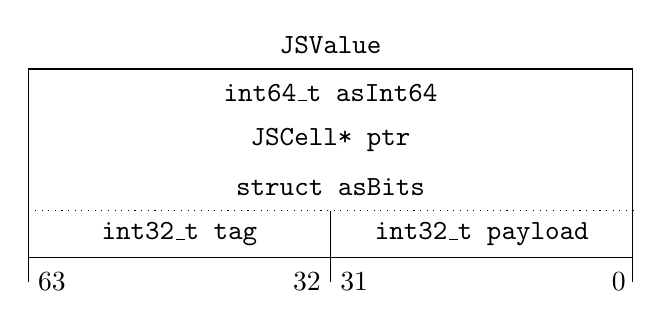
\begin{tikzpicture}[scale=.12]
 \draw[anchor=center] (32,2.5) node {\code{JSValue}};
 \draw (0,0) -- (0,-20) -- (64,-20) -- (64,0) -- cycle;
 \draw[anchor=center] (32,-2.5) node {\code{int64\_t asInt64}};
 %\draw[anchor=center] (32,-7.5) node {\code{double asDouble}};
 \draw[anchor=center] (32,-7.5) node {\code{JSCell* ptr}};
 %\draw (0,-10) -- (64,-10);
 \draw[anchor=center] (32,-12.5) node {\code{struct asBits}};
 \draw [dotted] (0,-15) -- (64,-15);
 \draw (32,-15) -- (32,-22.5);
 \draw[anchor=center] (16,-17.5) node {\code{int32\_t tag}};
 \draw[anchor=center] (48,-17.5) node {\code{int32\_t payload}};
 \draw (0,-20) -- (0,-22.5);
 \draw (64,-20) -- (64,-22.5);
 \node at (62.5,-22.5) {0};
 \node at (34.5,-22.5) {31};
 \node at (29.5,-22.5) {32};
 \node at (2.5,-22.5) {63};
\end{tikzpicture}
        \vfill
\end{minipage}
&
\begin{tabular}{c|l}
    bit values & type  \\
\hline
    \texttt{0000 0000 0000 0000} & \texttt{empty} \\
    \texttt{0000 0000 0000 0004} & \texttt{deleted} \\
    \texttt{0000 0000 0000 0002} & \texttt{null} \\
    \texttt{0000 0000 0000 0006} & \texttt{false} \\
    \texttt{0000 0000 0000 0007} & \texttt{true} \\
    \texttt{0000 0000 0000 000a} & \texttt{undefined} \\
    \texttt{0000 pppp pppp pppp} & \texttt{pointer} \\
    \texttt{0001 dddd dddd dddd} & \tikzmark{2nd} \multirow{3}{*}{\texttt{  double}} \\
    \texttt{\vdots} & \\
    \texttt{FFFE dddd dddd dddd} & \tikzmark{4th} \\
    \texttt{FFFF 0000 iiii iiii} & {integer}
\end{tabular}
\begin{tikzpicture}[overlay, remember picture]
    \draw [decoration={brace,amplitude=.5em}, decorate]
    ($(2nd)+(0,1ex)$) -- ($(4th)+(0,1ex)$);
\end{tikzpicture}

\end{tabular}
\caption{
    \label{fig:base-encoding}
    Representation of the internal \code{JSValue} class and the dynamic type encoding used in Webkit's JavaScriptCore VM.}
\end{figure}

\begin{comment}
         *     False:     0x06 =     4 + 2
         *     True:      0x07 =     4 + 2 + 1
         *     Undefined: 0x0a = 8     + 2
         *     Null:      0x02 =         2

         * These values have the following properties:
         * - Bit 1 (TagBitTypeOther) is set for all four values, allowing real pointers to be
         *   quickly distinguished from all immediate values, including these invalid pointers.
         * - With bit 3 is masked out (TagBitUndefined) Undefined and Null share the
         *   same value, allowing null & undefined to be quickly detected.
         *
         *     Deleted:   0x0
         *     Empty:   0x4
         * No valid JSValue will have the bit pattern 0x0, this is used to represent array
         * holes, and as a C++ 'no value' result (e.g. JSValue() has an internal value of 0).
        // These special values are never visible to JavaScript code; Empty is used to represent
        // Array holes, and for uninitialized JSValues. Deleted is used in hash table code.
        // These values would map to cell types in the JSValue encoding, but not valid GC cell
        // pointer should have either of these values (Empty is null, deleted is at an invalid
        // alignment for a GC cell, and in the zero page).
         */
\end{comment}

\subsection{Fat Value Technique}\label{sec:fat-values}
We can achieve dynamic information flow security by attaching, onto each runtime value, additional bits which encode a pointer, handle, or taint value representing the security type.
We term this technique the \term{fat value} approach, and extend the existing \code{JSValue} representation with an additional 64-bit word to hold the security type.
As shown in Figure~\ref{fig:fat-encoding}, each value within the interpreter then becomes 128-bits and contains both the originally encoded value and its security tag.

\begin{figure}[h]
\begin{minipage}[h]{.7\textwidth}
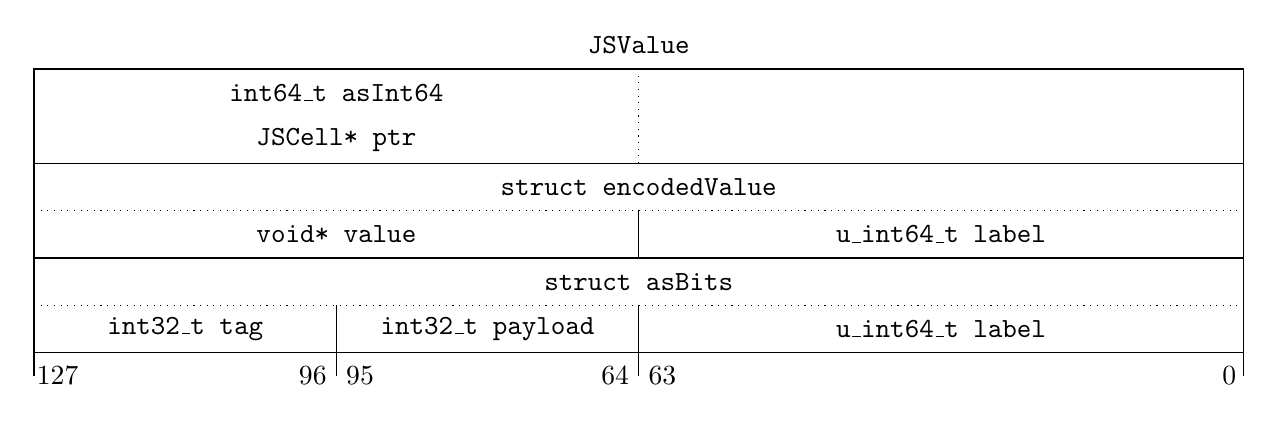
\begin{tikzpicture}[scale=.12]
 \begin{scope}[shift={(0,0)}]
 \draw (0,-5) rectangle (128,-15);
 \draw[anchor=center] (64,-2.5) node {\code{JSValue}};
 %\draw (64,-5) -- (64,-15);
 \draw[anchor=center] (32,-7.5) node {\code{int64\_t asInt64}};
 %\draw[anchor=center] (32,-12.5) node {\code{double asDouble}};
 \draw[anchor=center] (32,-12.5) node {\code{JSCell* ptr}};
 \draw[dotted] (64,-5) -- (64,-15);
 \end{scope}

 \begin{scope}[shift={(0,-15)}]
 \draw (0,0) rectangle (128,-10);
 \draw[dotted] (0,-5) -- (128,-5);
 \draw (64,-5) -- (64,-10);
 \draw[anchor=center] (64,-2.5) node {\code{struct encodedValue}};
 \draw[anchor=center] (32,-7.5) node {\code{void* value}};
 \draw[anchor=center] (96,-7.5) node {\code{u\_int64\_t label}};
 \end{scope}

 \begin{scope}[shift={(0,-25)}]
 \draw (0,0) rectangle (128,-10);
 \draw[anchor=center] (64,-2.5) node {\code{struct asBits}};
 \draw[dotted] (0,-5) -- (128,-5);
 \draw[anchor=center] (16,-7.5) node {\code{int32\_t tag}};
 \draw[anchor=center] (48,-7.5) node {\code{int32\_t payload}};
 \draw[anchor=center] (96,-7.5) node {\code{u\_int64\_t label}};
 \draw (32,-5) -- (32,-10);
 \draw (64,-5) -- (64,-10);
 \end{scope}

 \begin{scope}[shift={(0,-35)}]
 \draw (0,0) -- (0,-2.5);
 \node at (2.5,-2.5) {127};
 \node at (29.5,-2.5) {96};
 \draw (32,0) -- (32,-2.5);
 \node at (34.5,-2.5) {95};
 \node at (61.5,-2.5) {64};
 \draw (64,0) -- (64,-2.5);
 \node at (64+2.5,-2.5) {63};
 \node at (126.5,-2.5) {0};
 \draw (128,0) -- (128,-2.5);
 \end{scope}
\end{tikzpicture}
\end{minipage}
 \caption{Fat value encoding scheme.}
 \label{fig:fat-encoding}
\end{figure}\hfill

The fat value technique requires modifying the core representation of all values within the VM.
While performing this modification on an arbitrary dynamic language VM is not necessarily a trivial undertaking, the designers of JavaScriptCore have conveniently encapsulation the type inspection and conversion methods in the \code{JSValue} class.
This practice makes the modification easier than on other JavaScript VM's such as SpiderMonkey.
However, appropriately tagging each value with a security label still requires manual inspection of all code sites which create new values.
Additionally, doubling the size of the core datatype also doubles the memory space requirements of any running program: the VM allocates twice as much space for the same number of core values.

\subsection{Security Wrapper Technique}\label{sec:cloaks}

Another mechanism, known as the security wrapper technique, can also achieve the goal of attaching a security label to each value.
In this mechanism, the VM labels JavaScript objects by extending them with an additional internal field.
We introduce an internal security wrapper object which stores a primitive together with its label.
Throughout our analysis, we shall refer to this wrapper object as a \term{cloak} and any value held within the wrapper as a \term{cloaked} value.
Figure~\ref{fig:security-wrapper} provides a visualization of the cloak mechanism.

\begin{figure}[h]
 \centering
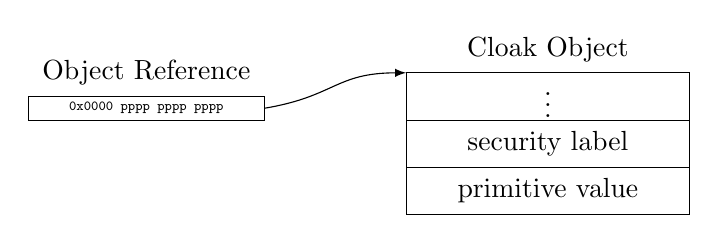
\begin{tikzpicture}[scale=.12]
    \node[anchor=center] at (12.5,2.5+2.5) {Object Reference};
    \node[anchor=center] at (12.5,2.5/2) {\tiny \texttt{0x0000 pppp pppp pppp}};
    \draw (0,0) rectangle (25,2.5);

    \coordinate (Obj) at (40,5);
    \node[anchor=center] at ($(Obj)+(15,2.5)$) {Cloak Object};
    \draw (Obj) rectangle ($(Obj)+(30,-15)$);
    \node[anchor=center] at ($(Obj)+(15,-2.5)$) {\vdots};
    \draw ($(Obj)-(0,5)$) -- ($(Obj)+(30,-5)$);
    \node[anchor=center] at ($(Obj)+(15,-5-2.5)$) {security label};
    \draw ($(Obj)-(0,10)$) -- ($(Obj)+(30,-10)$);
    \node[anchor=center] at ($(Obj)+(15,-10-2.5)$) {primitive value};

    \draw[-latex] (25,2.5/2) .. controls (25+15/2,2.5) and (25+15/2,5) ..  (Obj);

\end{tikzpicture}
\caption{Security wrapper scheme.}
\label{fig:security-wrapper}
\end{figure}

Internally, JavaScriptCore already supports wrapper classes for Strings and Dates, as well as automatic objection promotion for Numbers and Booleans.
Given this information, we might expect fewer modifications to be made to the underlying VM, as this change only requires the introduction of a new subclass of the existing \code{JSWrapperObject}.

However, implementing the wrapper class is not exactly trivial, even with the help of an existing framework.
From the perspective of the JavaScript program, a cloak object must mimic, in every circumstance, the same behavior as the primitive it cloaks.
Under no circumstances should the presence (or absence) of a security wrapper ever become evident to a JavaScript program, otherwise attacker provided code could exploit the difference in behavior.
%We make an exception to this guideline for policy violations, which have the side effect of halting the VM.
The wrapper must remain distinguishable to the VM, however, so that it can enforce information flow security.

Meeting this restriction is not presently possible using the existing wrapper framework.
The primary goals of the existing wrapper class is to collect those datatypes (Date, String, Number, and Boolean) which can be stored within the space of a \code{JSValue}.
As a result, the treatment of wrapped objects within the interpreter does not sufficiently take into account the behavioral differences between objects and primitives.
For example, in Listing~\ref{list:boolean}, a Boolean object wrapping the primitive value \code{false} behaves according to the rules governing objects rather than those of the primitive boolean value.
Consequently, the existing framework poses an imperfect fit for implementing information flow security, because it does not guarantee perfect transparency (from the perspective of a JavaScript program) when used to wrap primitives.

\begin{lstlisting}[caption={JavaScript considers objects as `truthy' values.},label={list:boolean}]
js> var x = new Boolean(false)
js> if (x) { print("x is true"); }
x is true
\end{lstlisting}

\section{Impacts on the Virtual Machine}
\label{sec:analysis}

Now that we have introduced two viable techniques for implementing information flow security, we analyze how each performs when labeling primitives, how each handles interned objects, and what impacts each has on the garbage collector.

\subsection{Labeling Primitives}\label{sec:primitives}

%Although the tagged pointer encoding is an implementation detail, this decision has had side effects which have leaked into the JavaScript specification.
%The foundational JavaScript VM, SpiderMonkey, initially implemented a tagged pointer encoding scheme for the 32-bit machines of that era.
%For example, SpiderMonkey's original 32-bit implementation used 1 bit for the integer type tag, and 31 bits for integer values.
%This design forced the language specification~\cite{ecma} to provide a coercion of any integer which cannot be represented by 31-bits to the \texttt{double} type.

The existing core datatype in JavaScriptCore uses a NaN encoding scheme that enables the value and type tag to coexist in the same memory structure.
The tagged pointer technique has the benefit of allowing the VM to perform operations on primitives quickly and directly.
Unfortunately, many common operators, such as \texttt{+}, behave differently depending on the types of the arguments.
Not only must the VM first inspect the type of the core values involved before dispatching the operation, but it then also unpacks the payload of the arguments from their encoding.

Using the fat value approach requires modifying the core value representation, extending it with additional bits to hold the security type.
This modification impacts the mechanisms used to encode and decode primitive values, as well as the type inspection routines.
JavaScriptCore uses an Object-Oriented design that encapsulates the type inspection logic, preventing it from dispersing across the VM implementation.
However, we must still manually audit each site at which the VM creates \code{JSValue}s so that the appropriate security label can be set.

Alternatively, the cloak approach requires the creation of a wrapper object for each labeled primitive.
Although the cloak easily holds both the core value representation of the primitive as well as the security type, the presence of a cloak object negatively impacts the runtime type inspection logic.
Where before the VM would previously inspect a primitive, it now dispatches inspection logic on a cloak object.
This extra layer of indirection severely degrades the performance of the very operations for which primitives are optimized.

The WebKit developers have designed JavaScriptCore as an embeddable interpreter.
Systems external to the JavaScript engine, such as the DOM framework of the WebKit browser, reflect their own classes into the JavaScriptCore engine.
This reflection occurs via a layer of interface classes\footnote{The WebKit build system automatically generates the interface classes.}, which each inherit a JavaScriptCore class such as \code{JSNonFinalObject}.
Should an external system expect certain fields to contain raw primitives (such as integers), it will fail when receiving a cloaked value.
When implementing the cloak scheme, we must either prohibit cloaks from escaping the JavascriptCore VM or modify the interface layer to automatically uncloak.
Both of these solutions leave the browser's external systems open as an information side channel.

To avoid observable semantic changes that could be exploited by an attacker, cloaks must also remain completely invisible to the JavaScript programmer.
For example, even though we implement cloaks as a native \code{JSObject} within the VM, we cannot allow a JavaScript program to set a property on a cloaked primitive.
Additionally, some JavaScript operators, such as \code{typeof}, require introducing an additional special case.
For example, a cloaked integer reports the type of the cloaked value, ``\code{number}'', rather than the type of the cloak, ``\code{object}''.
Should the VM use this operator internally for a type dispatch, it would then pass the value into a native routine expecting a raw primitive value.
To reduce the amount of implementation effort, we seek to avoid hunting down all the type dispatch sites and introducing these special cases.

When we compare the fat value approach to the cloak approach, an interesting semantic difference arises:
In the fat value approach, we attach the security type to the primitive value or object reference, as part of the tagged pointer encoding.
In the cloak approach, each object receives an internal field in store its security label while primitives are cloaked with an extra layer of indirection.

\todo{I haven’t fully explored the difference between having a labeled reference vs having a labeled object, but I think the difference is analogous to having an Access Control Listing by columns vs Object Capabilities by rows, as discussed in Capability Myths Demolished.}
% At this point I am in favor of the fat value approach, because I’m liking the reference semantics, and the transparency with which primitives can be labeled. I’m also willing to accept the cost of having fatter values.

\section{Implementation Experience}
\label{sec:experience}

\section{Related Implementations}
\label{sec:related-work}

\section{Chosen Implementation for FlowCore}
\label{sec:conclusion}


\chapter{Label Propagation}
\label{ch:label-propagation}

Web browsers which execute JavaScript code allow pages to load JavaScript and HTML code from many different sources into the same execution context.
This work distinguishes between JavaScript programs by tagging each with a different label representing its domain of origin.
Many web pages using this technique contain cooperating functions which generate shared objects.
Each object created or modified via the confluence of separate scripts bears a label which tracks all domains influencing the object.

\begin{figure}[ht]
  \centerline{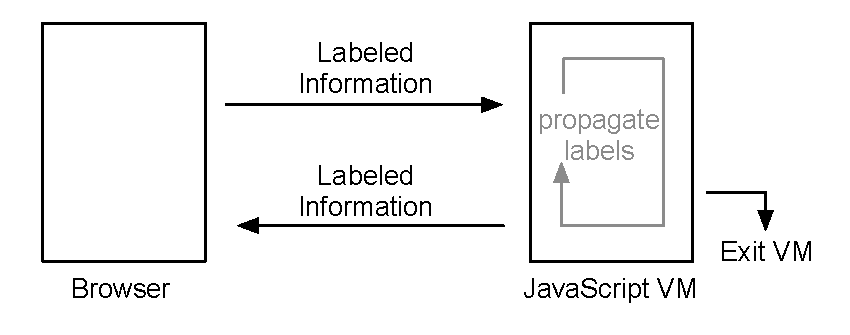
\includegraphics[keepaspectratio=true]{images/browserinteraction.pdf}}
  \caption{Interaction of the browser and the JavaScript~VM}
  \label{fig:browserinteraction}
\end{figure}

Figure~\ref{fig:browserinteraction} illustrates the interaction between the browser and the JavaScript engine.
Before the browser hands a script and its input data to the JavaScript VM, it first labels the script to indicate the domain of origin.
The VM then compiles the script source into an internal bytecode instruction representation.
During this process, static analysis enables the instrumentation of additional instructions that allow information flow tracking during execution.

\section{Label Lattice}
\label{sec:label-lattice}

This work takes inspiration from the decentralized label model~\cite{myers.liskov+00}.
Each web domain corresponds to a separate security principal, shown in the bottom row of Figure~\ref{fig:label-lattice}.
The information flow framework extends JavaScriptCore with a \code{LabelRegistry} which maps web domains to unique bit positions within the 64-bit label portion of a \code{JSValue}.
This configuration allows labels to represent any element within the lattice over web domains.
Figure~\ref{fig:label-lattice} depicts an example lattice for a page pulling JavaScript programs from three separate domains.

\tikzset{arrow/.style={
  decoration={markings,mark=at position 1 with {\arrow[scale=2.5]{latex'}}},
  postaction={decorate},
  shorten >= 0.4pt}
}

\tikzset{labarrow/.style={
  decoration={markings,
              mark=at position 0 with {\arrow[scale=1.5]{|};},
              mark=at position 1 with {\arrow[scale=2.5]{latex'};}
             },
  postaction={decorate},
  }
}

\tikzset{labelprop/.style={
  decoration={markings,mark=at position 1 with {\arrow[scale=2.5]{latex'}}},
  postaction={decorate},
  shorten >= 0.4pt}
}

\begin{figure}[ht]
\begin{tikzpicture}[node distance = 1cm, auto,
    force/.style={rectangle, inner sep=5pt, text badly centered, minimum height=.8cm}
    ]

    \begin{scope}[yshift=3.75cm, xshift=-7cm]
    \node[shape=rectangle, draw] {
       \begin{tabular}{l|c}
          \multicolumn{2}{c}{\code{LabelRegistry} mapping} \\
          \hline
          example.com & \texttt{0001} \\
          maps.com & \texttt{0010} \\
          ad.com & \texttt{0100} \\
       \end{tabular}
    };
    \end{scope}

    \begin{scope}
    \matrix[nodes={force}, column sep=1cm] {
        \node (ex) {example.com}; &
        \node (mp) {maps.com}; &
        \node (ad) {ad.com}; \\
    };
    \end{scope}

    \begin{scope}[yshift=2cm]
    \matrix[nodes={force}, column sep=.5cm] {
      \node (exUmp) {example.com $\sqcup$ maps.com}; &
      \node (exUad) {example.com $\sqcup$ ad.com}; &
      \node (mpUad) {maps.com $\sqcup$ ad.com}; \\
    };
    \end{scope}

    \begin{scope}[yshift=4cm]
    \matrix[nodes={force}, column sep=1cm] {
      \node (exUmpUad) {example.com $\sqcup$ maps.com $\sqcup$ ad.com}; \\
    };
    \end{scope}

    \draw[arrow] (ex) -- (exUmp);
    \draw[arrow] (ex) -- (exUad);

    \draw[arrow] (mp) -- (exUmp);
    \draw[arrow] (mp) -- (mpUad);

    \draw[arrow] (ad) -- (exUad);
    \draw[arrow] (ad) -- (mpUad);

    \draw[arrow] (exUmp) -- (exUmpUad);
    \draw[arrow] (exUad) -- (exUmpUad);
    \draw[arrow] (mpUad) -- (exUmpUad);

\end{tikzpicture}
  \caption{Interaction of the browser and the JavaScript~VM}
  \label{fig:label-lattice}
\end{figure}

Throughout execution, the modified JavaScript VM attaches the security labels to new JavaScript values based on the current execution context and web domain of origin.
Because labels can represent any element from the lattice, the interpreter is able to fully track which domains are involved in influencing each object.

\section{Label Operations}

The design decision to use a bit position encoding for web domains limits the framework to at most 64 domains.
Testing never encountered\footnote{Testing covered all pages within the \textit{Alexa Top 1000}~\cite{alexa}, but reloaded the browser for a clean slate between pages.} a single web page which included code from more than 64 different domains.
The framework contains no fundamental design flaws that would prevent an extension to the label encoding, if necessary.

\begin{definition}
  Given two security labels, $a$ and $b$, the {\bf join}, $a \sqcup b$, contains security principals that belong to the label $a$, the label $b$, or both.
\end{definition}

Using a bitwise representation allows the use of efficient bit arithmetic for computing the join (bitwise or) of two labels.
This operation occurs in every method call, assignment, and expression evaluation.
For example, when the program adds two numbers, the information flow framework labels the result with the join of the labels of the arguments and the label of the program counter.
Web applications today contain large amounts of JavaScript, which users expect to run without delay.
Label joining occurs frequently enough that any implementation other than bit arithmetic unacceptably penalizes the JavaScript runtime speed.

\begin{definition}
  Given two security labels, $a$ and $b$, the {\bf subsumes} relation, $a \sqsubseteq b$, is true if and only if the set of security principles comprising label $a$ is subset of the security principles comprising label $b$.
\end{definition}

The browser detects information leaks by comparing the label attached to a network request and the destination domain.
To assist with this task, labels support a subsumes relation that reveals the partial order of labels in the lattice.
If the label on the request contains principles other than the destination domain, the browser flags the request as a potential information leak.

\begin{definition}
  Given a security labels $a$ and $b$, the information flow VM {\bf upgrades} label $a$ with $b$ when it replaces $a$ with the join of $a$ and $b$, written $a \gets a \sqcup b$.
\end{definition}

When the Vm assigns value to an existing variable, it upgrades the label on the destination variable with the label attached to the source value.
Because assignment represents a mutation of memory, the VM also upgrades the destination label with the current \pclabel.
The labels faithfully record the dependence of the assignment on the current security context.

%TODO: include equal relation?
%TODO: include strict subsumption?

\section{Control Flow Stack}
\label{sec:control-flow-stack}

In a dynamically typed language such as JavaScript, the techniques of static analysis that rely upon static typing (developed in languages such as Jif~\cite{jif}) are inapplicable.
As a result, the information flow modifications to the JavaScript VM perform tracking up to active implicit information flows.
By handing back label information on values used in construction of a network resource request, the VM modifications increase the data available to the browser for making network policy enforcement decisions 
However, to prevent information leak to third parties, the browser ultimately remains responsible for enforcing a security policy on network traffic.

The syntax of JavaScript programs allows for points where the control flow branches due to the evaluation of a runtime conditional.
At each of these points, the security context of any code executed within the taken branch needs to reflect its dependence on the conditional.
To accomplish this task, we augment the JavaScript interpreter with a stack of labels, called the \term{control flow stack}.
As shown in Figure~\ref{fig:cf-stack}, the labels on this stack are in a 1-1 correspondence with the branches in control flow taken at runtime.
%This correspondence allows for tagging newly assigned values and function frames with the current security context.

\begin{figure}[ht]
  \centering
\begin{tikzpicture}[node distance = 0pt,
    box/.style={rectangle, draw, inner sep=3pt, text badly centered, minimum height=.8cm, minimum width=3cm},
    ]

%TODO: isn't there a split rectangle that I can use?

    \matrix[nodes={box}, anchor=south] (ops) {
      \node (condB) {conditional$_b$}; \\
      \node (condA) {conditional$_a$}; \\
      \node (func) {function call}; \\
      \node (dots) {\ldots}; \\
    };
    \node[below=of ops, align=center] {Operand and\\ Function Call\\ Stack};

    \matrix[nodes={box}, anchor=south, xshift=5cm] (labs) {
      \node (labFBA) {F $\sqcup$ C$_a$ $\sqcup$ C$_b$}; \\
      \node (labFA) {F $\sqcup$ C$_a$}; \\
      \node (labF) {F}; \\
      \node {\ldots}; \\
    };
    \node[below=of labs, align=center] {Control Flow\\ Stack};
    \node[right=of labFBA, align=left] {\pclabel};

    \draw[labarrow] ($(condB.mid east)+(.1,0)$) -- (labFBA.mid west);
    \draw[labarrow] ($(condA.mid east)+(.1,0)$) -- (labFA.mid west);
    \draw[labarrow] ($(func.mid east)+(.1,0)$) -- (labF.mid west);
    %\draw[labarrow] ($(dots.south west)+(-.3,0)$) -- +(0,4);
    \draw[arrow] (condB.north) -- +(0,.8);
    \draw[arrow] (labFBA.north) -- +(0,.8);

\end{tikzpicture}
  \caption{Correspondence of branches in control flow and labels of the control flow stack.}
  \label{fig:cf-stack}
\end{figure}

The control flow stack records the runtime sequence of labels attached to the program counter.
At all time the top of the control flow stack holds the label of the current program counter, \term{\pclabel}, identifying the security context of any operations currently under execution.
When the information flow VM assigns a value, it also joins the label attached to that value with the current \pclabel.

\subsection{Monotonicity of Control Flow Stack}

We use two guidelines for maintaining the control flow stack:
\begin{enumerate}
 \item Whenever control flow diverges due to an \code{if}, \code{while}, \code{for}, \code{switch}, function call or similar statement, the VM duplicates the top of the control flow stack to indicate entry into a secure region.
 \item Whenever a control flow joins, the VM pops and discards the top of the control flow stack, restoring the \pclabel\ to the value it had before the branch in control flow occurred.
\end{enumerate}

Of conspicuous absence in our guidelines (and the complete list of control flow stack instructions in \autoref{ch:instructions}) is an operation for pushing a specific security label onto the control flow stack.
According to the first guideline, the stack grows via successive duplications.
When the VM enters a secure code region it first duplicates the \pclabel\ and then joins it with the label attached to the condition which cause the control flow branch.
This execution directly implies an important theoretical result:
\begin{theorem}
  At all times during program execution, the control flow stack contains monotonically increasing security labels.
\end{theorem}
\begin{proof}
 Let $i$ be the index of a label on the control flow stack, and $L_i$ be value of that label.
 Let the base of the stack be at index $i=0$.
 There are three basic operations which modify the control flow stack:
 \begin{enumerate}
  \item A \textit{pop} decreases the size of the stack, but does not modify any labels currently on the stack. Any existing relation between consecutive labels remains unchanged.
  \item A \textit{dup} duplicates the topmost label and pushes it onto the stack. This operation implies that all labels on the stack are of equal security, $L_i~=~L_{i+1}$.
  \item A \textit{join} upgrades the top of the stack by replacing it with the join of the top and an arbitrary label representing the control flow branch. This operation weakens the previous equality, $L_i~\sqsubseteq~L_{i+1}$.
 \end{enumerate}
 We now directly observe that for all indices $i$ on the stack, $L_i~\sqsubseteq~L_{i+1}$, which is the monotonicity condition to be proved.
\end{proof}

\section{Label Creep}
When the information flow VM assigns to a value, it upgrades the label attached to that value with the current \pclabel\ (a.k.a. the top of the control flow stack).

The information flow VM system, explicitly labels values manufactured in a higher security context before allowing them to enter a lower security context, as may happen during via a function \code{return} statement.
The VM labels the result of computations involving two or more values using the join of the labels of all arguments.
The program counter acts as an implicit argument in all operations, so it's label too is joined in with the result.
As the interpreter executes, these joins steadily elevate the labels on objects within the system, a phenomenon known as \term{label creep}~\cite{sabelfeld.myers+03}.

At all times during program execution, a monotonically increasing list of security labels comprises the control flow stack.
All of the operations that our system performs on the control flow stack either leave the relationship between successive labels unchanged, or elevates the labels at the top of the stack.
Because all labels attached to values incorporate the current program counter label, which lies at the top of the control flow stack, it is important not to elevate the \pclabel\ unless absolutely necessary.
Otherwise, an overly-conservative \pclabel\ leads to the creation of values with unnecessarily elevated security labels.
This work therefore recognizes the monotonicity of the control flow stack to be the primary source of label creep.

Austin and Flanagan~\cite{austin.flanagan+12} give an example of indirect information flow and compare the published mitigation strategies.
Unfortunately, none of these solutions offers a silver bullet.
Two of the strategies~\cite{zdancewic+02,austin.flanagan+10} degrade user experience by halting execution to prevent passive implicit flows.
The third strategy~\cite{vogt.etal+07} uses a conservative labeling strategy that leads to label creep~\cite{sabelfeld.myers+03} in all but trivial cases.

\section{Formal Semantics}

\FlowCore\ tracks information flows across both kinds of explicit flows and active implicit flows.
When \FlowCore\ evaluates an expression, it tags the resulting value with a label indicating the principals that influenced its creation.

Guha et al.~\cite{guha.etal+10} reduce JavaScript to a succinct, small-step operational semantics that helps clarify \FlowCore's tracking capabilities.
I extend their notation to include security labels such that $x:l$ denotes an expression or value $x$ with the label $l$ and $l_1 \sqcup l_2$ represents the join (union) of principals represented by $l_1$ and $l_2$ respectively.

\subsection{Labeling Data Flow}

For all of the operations that it tracks (\autoref{ch:label-tracking}), \FlowCore\ labels the resulting value with a join over all of the labels on the input values.
The addition of two numbers constitutes an explicit information flow, as shown in \autoref{eqn:formal-addition}

\begin{equation}
\label{eqn:formal-addition}
  e_1:l_1 + e_2:l_2 \hookrightarrow v:l_1 \sqcup l_2
\end{equation}

\subsection{Labeling Control Flow}
\label{sec:formal-semantics}

Attackers can also generate implicit flows from confidential to public variables using the control-flow structures in JavaScript~\cite[p.~135]{guha.etal+10}.
The label of a statement within a branch acquires all the principals of the predicate controlling the branch in addition to the principals affecting the expression.
When the predicate evaluates to true, we have:

\newcommand{\kw}[1]{\text{\small\textsf{\textbf{#1}}}}

\begin{equation}
  \kw{if}\;(e_{true}:l_{pred})\;\{\;e_1:l_1\;\}\;\kw{else}\;\{\;e_2:l_2\;\} \hookrightarrow e_1:l_{pred} \sqcup l_1
\end{equation}

Since the tracking mechanism operates at runtime, it does not track passive implicit flows arising from control-flow branches that are not executed.

Loops act as a sequence of if-else branches, with each iteration dependant on a different predicate value during execution.

\begin{equation}
\begin{split}
  \kw{while}\;(e_1:l_1)\;\{\;e_2:l_2\;\} \hookrightarrow
  e_2:l_1 \sqcup l_2 ;\; &\kw{if}\;(e_1:l_1)\;\{\;
  \kw{while}\;(e_1:l_1)\;\{\;e_2:l_2\;\}\;\}  \\
  &\kw{else}\;\{\;\kw{undefined}:\bot\;\}
\end{split}
\end{equation}

Just as the value of the loop predicate may change between iterations, so also can the attached label.
However, the incorporation of the program counter as an implicit input to the loop predicate expression together with the absence of a declassification operation cause a monotonic increase on the label attached to the expression controlling the loop exit.
Consequently, each iteration executes under a label at least as high as the iteration preceding it.
Loop predicate expressions also act as a source of label creep.



\newcommand{\popj}{\code{POPJ\_CFLABEL} }
\newcommand{\dup}{\code{DUP\_CFLABEL} }
\newcommand{\join}{\code{JOIN\_CFLABEL} }

\chapter{Control Flow Instructions}
\label{ch:instructions}

Typically, a host application which supports an embedded programming language does so to increase end-user functionality. 
For example, a web browser supports JavaScript to enable more interactive pages.
At the time developers introduce the ability to program their application, focus usually rests on extending existing functionality rather than any security implications raised by the ability to run user provided programs.
Side-effects of this prioritization can be seen in today's web ecosystem.

Because of an early and rapid rise in electronic commerce, web browsers now often manipulate, process, and relay sensitive information, including personal financial data.
A browser's support for JavaScript means that it is possible for malicious code to steal the valuable information stored by the browser.
Recall that web browser architecture lacks (and sometimes impedes) important security properties (Section~\ref{ch:motivation}).
This state of affairs makes web sites a prime target for injected code attacks.
Consequently, the combination of historically poor security practices and the popularity of the web makes web browsers an ideal case study for retrofitting security into embedded language platforms.

Rather than fret over distinguishing between legitimate and malicious code (or buggy legitimate code), FlowCore performs information tracking on all executed code.
This approach catches all malicious behavior defined by some security policy (Section~\ref{policy}), forcing conformance even on trusted code.
FlowCore adds information flow tracking infrastructure to JavaScriptCore.
The retrofitting of security into an established and mature VM occurs as two components:
(1) labeling of the data types (Section~\ref{ch:system-design}) and 
(2) the instrumentation of instructions for managing runtime data structures such as the control flow stack (Section~\ref{sec:control-flow-stack}).
This chapter addresses the design of the instrumented instructions.

\section{The Necessity for New Instructions}

During initial implementation, I first attempted to manipulate the control flow stack by modifying the functionality of existing instructions.
However, this approach met with several obstacles which motivate the introduction of new security instructions.
These obstacles are not specific to either JavaScriptCore or SpiderMonkey, but originate from fall-through execution paths common to many languages.
The technique of extending the instruction set generalizes to other dynamically typed language runtimes.

When examining the instruction stream, the merge point of an \texttt{if-then-else} construct has no special distinguishing feature.
In some paths, a jump instruction targets the merge point, while in other paths execution arrives at the merge point via a fall-through.
Additionally, the instruction present at the merge point could be any of the existing instructions implemented by the VM.
Neither the instructions comprising the arrival path nor the instruction at the merge point itself can serve as a unique marker for identifying a merge point.
Because no runtime mechanism can identify the merge point based solely on a single path's sequence of executed instructions, FlowCore instruments a \popj instruction at every merge point.
Not only does this instruction serve as a marker which locates the merge point, but it also performs the appropriate action on the control flow stack.

A more subtle difficulty occurs at the beginning of conditional branch and loop structures.
Primitive underlying compare-and-jump instructions serve to easily identify these these points.
Examination of the target offset of the jump instruction can even distinguish loops from a conditional branch.
Loops have a backward branch (negative offset) while all conditional branches point forward (positive offset).
Naively, I thought it might be possible to modify the behavior of the compare-and-jump instructions to push a label onto the control flow stack.
However, this approach produces an erroneous execution in loops: every iteration in a loop evaluates the conditional instruction, causing a push which breaks alignment of the control flow stack with respect to the execution history of program counter.
To ensure that only one label push occurs at entry into a loop, FlowCore instruments a \dup instruction in the loop header.

Given the introduction of two instructions for manipulating the control flow stack, the FlowCore framework can now reliably keep the 1-1 correspondence between labels on the stack and branches in control flow taken at runtime.
However, the evaluation of a conditional instruction also implies an upgrade to a new security context.
To satisfy this additional requirement, FlowCore introduces the \join instruction, which upgrades the label on the top of the control flow stack using the label conditional controlling the branch.
Inserting this instruction between the computation of a conditional value and its use as a control flow branch allows both looping and branching constructs to compute the correct security context.

Treatment of return statements requires further analysis
FlowCore must take care to align the control flow stack height in the event that a return occurs inside a nested code block.
A translation of the return into a three step process accomplishes this task.
First, label the return value using the current top of the control flow stack (i.e. the pc-label) and cache the value in the stack frame.
Second, instrument a \popj to restore the control flow stack height.
Third, return the properly labeled value and tear-down the function.
In a register machine, such as JavaScriptCore, the return instruction implementation can perform all three steps, by extending the return instruction opcode with an immediate value representing the control flow stack depth.

\section{Security Instruction Details}

The JavaScript VM first compiles each script into an instruction stream before beginning interpretation.
FlowCore modifies the parser to produce an instruction stream that differs only by the addition of control flow instructions which track and record control flow paths executed at runtime.
During parsing, a static analysis provides the instruction emitter knowledge of nesting levels and control flow depth.
This information determines the values of parameters which control the number of pushes, pops, or joins carried out by the control flow stack at runtime.
To ensure that the parser performs instrumentation correctly, an abstract interpreter verifies, over all possible paths, a consistent control flow depth for each instruction in the stream.
Using the instrumented instructions at runtime, FlowCore maintains a 1-1 correspondence between the number of labels on the control flow stack and the number of control flow branches taken during program execution.

\lstset{caption={Hypothetical information leak of secret variable \code{pin}, using an active implicit information flow.},
        label=list:steal-pin}
\begin{jscode}
function steal_pin() {
  for (var i=0; i < 100000; ++i) {
    if (i == pin) break;
  }
  return i;
}
\end{jscode}

The code sample in Listing~\ref{list:steal-pin} contains control flow structures, such as a \texttt{for}-loop, \texttt{break} statement, and \texttt{return} statement which allows us to examine the placement of the security instructions in greater detail.
An attacker manages to inject the \code{steal\_pin} function, manufactured so that, at the end of execution, the local variable \code{i} contains the same value as the secret variable \code{pin}.

Despite the fact that other, more direct mechanisms can achieve this relationship, the example highlights lesser used control flow constructs, such as the \texttt{break} statement, and the impact these constructs have on maintaining the control flow stack height.

\begin{figure}[h]
\begin{python}
code = r'''
function steal_pin() {
  for (var i=0; i < 100000; ++i) {
    if (i == pin) break;
  }
  return i;
}

print(debug(steal_pin))
'''
import sys
sys.path.append('..')

import jsc
j = jsc.jsc(code)
j.run()

import bytecodeformatter
bytecodeformatter.tikz_picture(j.instructions())
\end{python}
  \caption{FlowCore instruction stream representing the code snippet in Listing~\ref{list:steal-pin}.}
  \label{fig:steal-pin-bytecode}
\end{figure}

\subsection{\dup}

\begin{samepage}
\begin{description}
  \item[Operation] \hfill \\
    Duplicate the top label of the control flow stack.
  \item[Control Flow Stack] \hfill \\
    \ldots, label, $\Rightarrow$ \ldots, label, label
\end{description}
\end{samepage}

The \dup instruction duplicates the top of the control flow stack.
FlowCore places this instruction before every control flow branch.
In many cases, this instruction pairs with a \join instruction which then upgrades the top of the control flow stack after evaluating the boolean condition of the branch.
In all cases, a corresponding \popj instruction later delineates the end of the secure region.

As shown in Figure~\ref{fig:steal-pin-bytecode}, the loop header of the code in listing~\ref{list:steal-pin}, occurs after the loop body.
A \dup instruction at offset~\code{01} occurs prior to evaluation of the loop initialization code.
The presence of this instruction prepares the control flow stack for the secure region delineated by the loop.
A corresponding \popj instruction at offset~\code{41} occurs on a fallthrough out of the loop restoring the control flow stack height.
A second secure region, delineated by the \code{if}-statement inside the loop, can be found with a \dup instruction at offset~\code{07} and its corresponding \popj instruction offset~\code{27}.

% Was true in Firefox, but not true in FlowCore
% As can be seen at offset , our system also inserts an additional \texttt{DUP\_CFLABEL} instruction at the beginning of every function.
% This instruction provides each function with an additional label on the control flow stack that clearly delineates the function boundary, and provides an explicitly labeled operating context for all calculations performed within the function body.
% Before the function returns, a corresponding \texttt{POP\_CFLABEL} instruction (line~\texttt{56}) restores the state of the control flow stack.



\subsection{\join}
\label{sec:join-cflabel}

\begin{samepage}
\begin{description}
\item[Operation] \hfill \\
 Upgrade the label at the top of the control flow stack by performing a lattice join with the label of the topmost value of the operand stack.
\item[Control Flow Stack] \hfill \\
 \ldots, label\subscript{a} $\Rightarrow$ \ldots, label\subscript{a} $\sqcup$ label\subscript{b}
\end{description}
\end{samepage}

A \join instruction supports upgrading the label of the program counter by joining the top of the control flow stack with the label of a given value.

This instruction is necessary for supporting loop structures that continue or exit based on a boolean condition evaluated at runtime.
Because the condition depends on a runtime evaluation, each iteration through the loop may carry a different security label.

Our system retains the successive joins of all iterations as it progresses through the loop.
A side effect of this design means that the evaluation of last iteration in a \code{for}-\code{in} loop over an array might occur under a higher security label than the first iteration.
For example, this situation occurs when the array consists of heterogeneously labeled fields.
Although finding ways to prevent such joins is worthy of further research, I speculate that doing so safely would require analysis proving non-interference between successive iterations.

In the running example (Figure~\ref{fig:steal-pin-bytecode}, the \join instruction at offset~\code{36} takes care of upgrading the current execution context at each iteration of the \texttt{for}-loop.
For the simple loop given in the example, upgrading the top of the control flow stack is wasteful, because every iteration occurs under the same security context.
FlowCore does not currently perform a more extensive analysis that would help identify this situation and optimize the join away.
Inside the \texttt{for}-loop, a \join instruction at offset~\code{17} upgrades the program counter based on the condition of the \texttt{if}-statement.

Note that incrementing the loop index variable (offset~\texttt{30}) occurs outside the context of the inner \texttt{if}-statement.
Even though we, as programmers, can see that the \code{break} statement enforces a dependence of the loop index variable on the secret variable \texttt{pin}.
FlowCore therefore contains another instruction which enables tracking this dependence over the \code{break} statement.

\subsection{\popj}

\begin{samepage}
\begin{description}
\item[Operation] \hfill \\
 Pop $p$ labels from the top of the control flow stack, then perform a lattice join on each of the next $j$ labels on the control flow stack with the previous topmost label.
\item[Control Flow Stack] \hfill \\
  \ldots, label\subscript{i}, label\subscript{i+1} \ldots, label\subscript{i+j}, label\subscript{i+j+1}, \ldots, label\subscript{i+j+p}\\
 $\Rightarrow$
 \ldots, label\subscript{i}, label\subscript{i+1} $\sqcup$ label\subscript{i+j+p}, \ldots, label\subscript{i+j} $\sqcup$ label\subscript{i+j+p}
\end{description}
\end{samepage}

The \popj security instruction carries two parameters: $p$, which specifies how many levels of control flow to pop, and $j$, which specifies how many further control flow levels that should be upgraded.
When the interpreter encounters a \popj instruction, it first saves the current top of the control flow stack, then it pops $p$ levels, and finally in-place joins $j$ more levels using the previously saved top.

In its primary role, the \popj instruction marks the position of every control flow merge and serves to pop a label from the control flow stack.
In the event that many control flow paths merge at the same point, the \popj instruction carries a parameter $p$, which indicates how may merges coincide.
For example, this situation may occur during an early return from within a nested loop.

In the example shown in Listing~\ref{list:steal-pin}, both the \code{for}-loop and the \code{if}-statement each require only a single label to be popped from the control flow stack.
The \popj instruction at offset~\code{41} marks the end of the \code{for}-loop and the \popj instruction at offset~\code{27} marks the merge point of the \code{if}-statement.
Both of these occurrences pop a single secure lexical region from the current control flow stack, restoring it to the height it had prior to entry of the control structure, according to the rules in Section~\ref{sec:control-flow-stack}.

The presence of the second argument, $j$, which gives a depth of how many further control flow scopes should be upgraded after popping, enables FlowCore to correctly handle \code{break} and \code{continue} statements.
These statements cause a divergence in control flow from within a nested scope out to a lexical outer scope.
As shown in the example in Listing~\ref{list:steal-pin}, the \code{break} statement enforces a equality of the secret variable, \code{pin} and the loop index variable, \code{i}.
Having established this relationship, the malicious code can pilfer information via the variable $i$ because JavaScript semantics cause loop index variables declared with the \code{var} keyword to be promoted to function-level scope.
As a result, FlowCore conservatively upgrades the entire function context via the joining operation incorporated into the \popj instruction.

When the nested \code{break} statement executes (Listing~\ref{list:steal-pin}), the control flow stack contains three labels: one for the function, one for the \code{for}-loop, and one for the \code{if}-statement.
As shown in Figure~\ref{fig:steal-pin-bytecode}, prior to exiting the loop due to the \code{break} statement, a \popj instruction at offset~\code{22} adjusts the control flow stack by popping the label of the \code{if}-statement (parameter $p$=1) and upgrades both the \code{for} loop and the current function scope (parameter $j$=2).
The \code{for}-loop then exits and the interpreter pops one label from the control stack (offset \code{41}), leaving only the label for the function scope left on the stack.

As noted previously, the inner \code{if}-statement does not directly influence the label attached to the loop index variable,~\code{i}.
Without upgrading this label, the \code{return} at offset~\code{44} of Figure~\ref{fig:steal-pin-bytecode} leaks the information of the secret variable \code{pin}.
However, the \popj instruction at offset~\code{22} upgrades the entire function context.
So any operations taking place after the occurrence of the \code{break} statement execute under a label at least as secure as the scope in which the \code{break} resides.
In particular, the \code{ret} instruction at offset~\code{44} executes under the upgraded label.
FlowCore modifies the \code{ret} instruction to upgrade the label of the returned value by joining it with the label of the current execution context.
This action prevents tracks the information flow demonstrated by Listing~\ref{list:steal-pin}.





\chapter{JavaScript Feature Catalog}

JavaScript, like many scripting languages, agglomerate different programming paradigms and hosts a large number of built-in conveniences.
In order to provide a comprehensive overview of the labeling semantics, this chapter gives the labeling semantics for each language feature present in JavaScript.

\section{Primitives}


\section{Data Structures}
\subsection{Objects}
\subsection{First-Class Functions}
\subsection{Built-ins}
\subsubsection{Arrays}
\subsubsection{Date}
\subsubsection{Interned Strings (And Other Things)}

\section{Control Flow}
\subsection{Function Calls}
\subsubsection{Closures}
\subsection{Early Return}
\subsection{Break and Continue}
\subsection{Exceptions}
\subsection{Eval}


 - what to do with arrays, or does this fit better in design considerations?
   : Can coalesce labels on arrays?
   : label bounds checking? 
 - obj literals
   how they interact with obj poisoning attack
 - retrieval
   indexing syntax [] vs .
   prototype chain
 - Seth Just Information flow analysis for JS has a good discussion about control flow structures.
 - early returns (out of nested loops)
 - break/continue (in nested loops)

%%%%%%%%%%%%%%%%%%%%%%%%%
% From 2011 acsac.tex

Although dynamically typed languages present many difficulties for ensuring information flow, we find that JavaScript uses structured control flow constructs.
As a result, we can use a static analysis which calculates exactly at which points our security instructions should be inserted into the instruction stream.
This modification allows our system to prevent implicit information flow leaks by tracking the security label of the program counter at runtime, using the control flow stack.
%Because local variables cannot leak information, allowing them to automatically upgrade still complies with the intention of non-interference security~\cite{goguen1982security}.
%Variables which can leak information are subject to the \textit{no sensitive upgrade} check (see Section~\ref{sec:sensitive-upgrade-check}), and are prevented from automatic upgrade.
%Using these principles, we demonstrate the labeling strategy for several control flow structures defined in the JavaScript language~\cite{ecma}.

\subsection{Conditional Branches}
Conditional branches begin with a \texttt{DUP\_CFLABEL} instruction that marks the beginning of a secure code region by cloning the current pc-label.
The conditional value itself may be the result of an arbitrary expression, which could include function calls and shortcut evaluation of logical operators.
Consequently, its label is not predictable at compile time, so we emit a \texttt{JOIN\_CFLABEL} instruction immediately following the conditional evaluation.
This instruction upgrades the top of the control flow stack using the label of the conditional value computed at runtime.
When either side of the conditional branch finishes executing, a \texttt{POP\_CFLABEL} instruction at the control flow join restores the pc-label to its state before the branch was encountered.

\subsection{Loops}

Because of the implied backwards branch, loops require more care than conditional branches.
Prior to entering the loop a \texttt{DUP\_CFLABEL} instruction clones the current pc-label.

Again, because the condition is a runtime evaluated expression, only a dynamic analysis can identify the correct label to apply to the loop body.
The possibility of an earlier iteration influencing a later iteration complicates the situation.
Our implementation emits a \texttt{JOIN\_CFLABEL} instruction at the end of the conditional, despite the fact that this forces the current pc-label to be re-upgraded at each iteration.
Upon exiting the loop, a \texttt{POPJ\_CFLABEL} instruction restores the pc-label to its state before the loop was encountered.

One caveat of this solution is that it allows a monotonically increasing label on the loop body.
It is unfortunately possible that later iterations may carry a higher pc-label than earlier iterations, even when these iterations do not influence each other.
For example, an array might contain a sequence of completely unrelated values, each cloaked with a different security label.
When looping over such a construction, our implementation does not downgrade the loop context, even if independence of iterations could be proven.

\subsection{Break and Continue}
\label{sec:break-and-continue}
JavaScript allows the \texttt{break} and \texttt{continue} statements to specify which loop they apply to.
This complicates the maintenance of a control flow stack, because such statements may jump out of an arbitrarily nested loop.
Such jumps can bypass the normal exit criteria of nested loops, thereby causing the control flow stack to be out of alignment at the target location.
To maintain correct runtime-behavior we must handle this issue by ensuring that the instruction emitter generates the correct number of control flow pops for any nested loops that are exited.
A static analysis in the parser performs this computation and provides the resulting number as a parameter to the \texttt{POPJ\_CFLABEL} instruction.

Loop index variables, which are commonly bound to the function scope\footnote{JavaScript binds variables declared with \texttt{var} to the function scope, and did not have a block level scope prior to the introduction of \texttt{let} in version~1.7.} can be used for an implicit information leak if they are not all upgraded to the current pc-label at the time a \texttt{break} or \texttt{continue} statement is encountered.
Our system prevents potential implicit information leaks by emitting a \texttt{POPJ\_CFLABEL} instruction that not only pops the correct number of control flow labels, but also takes care to upgrade the control flow stack for the current function.
Upgrading the control flow stack in this manner upgrades all the values present on the operand stack at the time the interruption in control flow occurred.
Any later computations performed by the function are then considered to be influenced by the security context in effect at the time the \texttt{break} or \texttt{continue} statement was encountered.

\subsection{Exceptions}
\label{sec:exceptions}
Exceptions represent a substantial challenge to information flow security, because a \texttt{throw} permits any called function to create an early return that crosses multiple function boundaries.
To complicate security issues further, JavaScript supports the \texttt{try}, \texttt{catch}, \texttt{finally} triplet of keywords.

The exception handling region of the \texttt{try}-block begins with a \texttt{DUP\_CFLABEL} instruction.
As a conservative precaution, when the interpreter encounters a \texttt{throw} statement, it takes care to first cloak the exception object that is to be returned to the exception handler using the current pc-label.
Once the interpreter finds the appropriate handler, it pops all activation frames within the call chain.
Control flow then transfers to the corresponding \texttt{catch}-block where a \texttt{POPJ\_CFLABEL} instruction upgrades the entire control flow stack of the handling function using the label taken from the exception object.
Taking this action prevents implicit information leaks that might occur due to exiting the \texttt{try}-block early.
Such leaks are analogous to the \texttt{break} and \texttt{continue} (see Section~\ref{sec:break-and-continue}).

The \texttt{finally}-block always executes using the current pc-label, which is provided either by finishing the \texttt{try}-block or from catching an exception and executing the \texttt{catch}-block.

\subsection{Function calls}
\label{sec:function-calls}
We found it unnecessary to introduce additional instructions to handle function calls.
Instead, we instrument the existing routine for a function call to lookup the label of a function at call time.
When a function call occurs, our system first duplicates the top of control flow stack then joins it with the label of that function.
This action makes all operations which occur within the body of that function safe.
The location of this label breaks down into three cases:
\begin{description}
 \item [The function is provided by a script.]
  When the host environment hands a script to the JavaScript VM, it has the option of labeling that script with a security principal.
  In this case, the function lookup process is responsible for retrieving the label of the function.
 \item [The function is an uncloaked first class value.]
  The current program counter implicitly labels anonymous functions at the time of their creation.
  As a result, the label of the function is always lower than that of the pc-label, and it is safe to call directly.
 \item [The function is a cloaked first class value.]
  If a sensitive control flow computation resulted in the return of a function, the return specification (see Section~\ref{sec:returns}) cloaks the function.
  In this case, the VM retrieves label of the function from its wrapper before the call.
\end{description}

\subsection{Returns}
\label{sec:returns}
A returned value needs to carry information indicating the security context under which the value was produced.
Our system achieves this by explicitly cloaking the return value with the current pc-label using \texttt{CLOAK} instruction.
%\todo{more? if value is already cloaked...}

\subsection{Eval}
\label{sec:eval}
Our system treats \texttt{eval} similar to other function calls.
In this case, the parameter string passed into the \texttt{eval} provides the label for the new execution context.
A call to \texttt{eval} first compiles this string into an instruction stream.
As a result of passing through the parser, this stream contains all of the security instructions as would a normal script.

%The \texttt{eval} frame performs variable access using dynamic lookup.
%The bytecodes emitted for these lookups are the same as the bytecodes emitted for a parent lexical scope (equiv. to global) accesses.
%Our system already mediates the modification of such variables using the \textit{no sensitive upgrade} check (see Section~\ref{sec:sensitive-upgrade-check}), so no extra precautions are necessary for securing the \texttt{eval} construct.

%===============================================================================

\section{Evaluation}
\label{sec:evaluation}

%
%To evaluate our claims we modified SpiderMonkey, the JavaScript VM used in the Mozilla Firefox browser.
%We examine the bytecode overhead introduced by the inclusion of the secure bytecodes, as well as its affect on usability.
%Based on our results from browsing real websites, we give some insight into the architectural changes website authors might have to make to support information flow security.

Our implementation focuses mainly on the creation of a fully functional and correct information flow tracking system.
We would like to note that, to the best of our knowledge, no standard set of tests for information flow frameworks currently exists.
Given this situation, we use the SunSpider~\cite{sunspider} benchmark suite to assess the overhead which our framework introduces.
Despite the fact that it does not faithfully represent real-world JavaScript~\cite{jsmeter}, we choose this suite because its status as the standard benchmark suite for JavaScript makes it suitable for comparisons to other work.

\subsection{Growth of Instruction Stream}
%\begin{figure*}[ht]
%  \centerline{\includegraphics[width=18cm,keepaspectratio=true]{graphics/evaluation_bytecodes.pdf}}
%  \caption{Bytecodes emitted for SunSpider benchmark}
%  \label{fig:eval_bytecodes}
%\end{figure*}

%Figure~\ref{fig:eval_bytecodes} shows the number of emitted bytecodes for each test in the SunSpider benchmark.

To examine impact that introducing the new security instructions has on the memory requirements of SpiderMonkey's internal bytecode representation, we measure the change in size of the emitted instruction stream, for each test in the SunSpider~0.9.1 benchmark suite.
Despite the fact that SunSpider runs only with only a single security principal, we find it useful for measuring the overhead incurred by introducing additional security instructions to well-known algorithms.

% secure = [178, 15, 158, 25, 48, 38, 25, 8, 14, 3, 20, 29, 181, 71, 87, 140, 183, 18, 6, 28, 4, 36, 32, 129, 83, 32]
% total = [ 2238, 173, 2446, 213, 334, 668, 164, 94, 81, 26, 167, 154, 2957, 1753, 930, 1313, 1556, 238, 195, 278, 144, 794, 325, 569, 592, 360]
% data = zip(secure, total)
% d = [ float(x[0]) / (x[1] - x[0]) for x in data ]
% d[8], d[11], d[23], (sum(d)/len(d))
We observe that tests such as \textit{string-tagcloud}, \textit{bitops-bit-in-byte} and \textit{controlflow-recursive}, which contain very ``branchy'' code with respect to their short length, incur the highest overhead; 29.3\%, 21.0\%, and 23.2\% respectively.
Control flow constructs feature much less prominently in the other SunSpider tests, so the introduction of instructions which track branches and merges incur a much lower overhead.
Inserting our security instructions into the instruction stream never causes it to grow by more than 30\%, and maintains an average overhead of 11.6\% growth.

We therefore feel it important to note that many optimization opportunities for reducing the overhead of our techniques remain available for future work.
For example, the overhead of introducing these instructions can likely be optimized away by using a runtime analysis to type-specialize over the labels on arguments and functions.
%Such techniques are very common among interpreter-based virtual machines to optimize ordinary operations.
%For the future however, we plan to follow the quickening approach so that our framework starts executing a bytecode-stream that includes the secure instructions and can jump to an unmodified bytecode-stream whenever possible.

\subsection{Effect on Performance}
\label{sec:evaluation-performance}

We executed the SunSpider~0.9.1 benchmark suite on a Quad Core Intel Xeon~5140 running at 2.33~GHz with 32GiB~RAM running Linux kernel~2.6.3.2.
To achieve a stable basis of comparison, we execute each test in the suite 100 times, and take the average over all runs.

Our modified version of SpiderMonkey requires 140 seconds to execute the entire benchmark, while an unmodified version requires only 22.5 seconds.
We compile both versions using the same flags.
This test demonstrates an overhead of approximately 6x, primarily due to the introduction of explicitly cloaked values at return sites.

Since each cloak is itself a JavaScript object, our system generates a much larger number of objects than an unmodified system, and thus spends more time doing object allocation and garbage collection.
Currently, SpiderMonkey uses an unsophisticated mark-and-sweep garbage collector and does not employ generational collection.
Recent improvements to the garbage collector~\cite{wagner2011} have already demonstrated a remarkable increase in collection speed, which will likely benefit our implementation.
We also believe that we can reduce the number of cloak objects and improve our implementation by using techniques such as sparse labeling~\cite{1554353,1814220}.
%Specifically, we expect to see a large performance improvement by placing objects into a labeled compartment within the garbage collector.

%We also visited several websites, to evaluate this performance overhead as it would appear to a casual user.
%When browsing the web with our system, we did not notice any slowdown for ordinary pages.
%However, we did notice a slight response delay when interacting with JavaScript heavy applications (such as GMail).

\subsection{Violations Issued when Browsing the Web}
We implement enough of the security framework that we can compile and run the Firefox browser.
Although we modify the SpiderMonkey interpreter to track information flow, we found that Firefox uses JavaScript internally for a large number of subsystems (including the user interface).
Despite the potential for covert channels, we chose to whitelist the classes involved in these subsystems and consider them a portion of the trusted code base.


We also used our modified version of Firefox to visit the top 10 sites in the \textit{Alexa's Top Sites}~\cite{alexa} listing.
During this test, our system detects a large number of information flow violations.
Figure~\ref{fig:eval_falsepositives} highlights the total number of unique violations issued for each of these pages.
Manual investigation reveals that the vast majority of these sites load images and other resources from a separate server.
Because sites request these resources from a domain different than the site itself, our system triggers an alarm due to the interaction of DOM objects having separate labels.
For our approach to be adopted in a working environment, web site authors clearly need a policy specification framework (further discussed in Section~\ref{sec:policy_specification}), so that they can express their site's trust in a content distribution server.

\todo[inline]{Figure of false positives}
\begin{comment}
\begin{figure}[htp]
  \centerline{\includegraphics[width=12cm,keepaspectratio=true]{graphics/evaluation_falsepositives.pdf}}
  \caption{Information flow alarms triggered when browsing Alexa's Top Sites in the United States~\cite{alexa}.}
  \label{fig:eval_falsepositives}
\end{figure}
\end{comment}

\subsection{Verification}

In addition to the evaluations presented above, we also implement 173 private test cases to ensure that we generate the correct labels for each of the control flow structures mentioned in Section~\ref{sec:program-control-structures}.
Our system is correctly able to identify both explicit and implicit information flows represented in this test suite, including the two examples presented in Figure~\ref{fig:threat_if} and Figure~\ref{fig:threat_for}.
Although this effort does not substitute for a proof of correctness, it does give us confidence that our implementation faithfully follows the approach we have outlined.

Our system also runs an abstract interpreter that verifies the control flow stack height at every instruction of a method.
This analysis covers \emph{all} possible executions paths for every method parsed, and ensures that we never introduce security instructions that might cause a runtime misalignment of the control flow stack.
We are able to run this verification over all of the more than 2,000 tests in the SpiderMonkey testing suite, which Mozilla uses to detect regressions for every code change.

%\todo{address reviewer comment: Performance overhead is reasonable, some benchmarks using real-world applications would be useful to estimate the actual impact on a system}

%===============================================================================


\todo[inline]{pull citations from acsac-tr}

\todo[inline]{remove the word 'bytecode' and 'opcode', replace with instruction}
\todo[inline]{remove security instruction, replace with control flow instruction}


\chapter{First-Class Labels}
\label{ch:first-class-labels}

The interpreter portion of \JitFlow\ forms the foundation of an information-flow tracking web browser that tracks flow in the Document Object Model, named ConDOM~\cite{kerschbaumer.etal+12}.
A modification of the ConDOM browser that randomly switches the information flow tracking capabilities on and off later formed a critical component of a system, called CrowdFlow~\cite{kerschbaumer.etal+13}, that gathers attack statistics across a crowd of users.

Concordant with our attack model (\autoref{ch:defense}), these systems also define an \emph{information leak} as the communication of any information to a web origin that differs from the flow-tracked derivation of that information.
Through automated browsing, ConDOM and CrowdFlow discovered a high number of false positives, where the web application sourced much of its material from Content Distribution Networks (CDNs) that have different domains than the page itself.

These observations indicate that JavaScript program authors have more knowledge about the information-flow security needs of the application they develop than any automated system can assess~\cite{hennigan.etal+12, hennigan.etal+13}.
To combat label creep and preempt the ex-post suggestion of applying a policy that whitelists CDNs, \JitFlow\ exposes some of the internal labeling operations through a first-class language feature.
Using this API, the JavaScript programmer, armed with domain knowledge, gains the ability to tag specific, security sensitive, values within their application.
By reducing the number of sources for labels, the developer can delay and mitigate the encroachment caused by label creep.

In addition to the tracking capabilities already outlined, \JitFlow\ also presents reflective \FlowLabel\ objects to interface with an internal \FlowLabelRegistry\ that holds the label lattice (\autoref{sec:label-lattice}).
The \FlowLabel\ objects themselves come equipped with \mjoin\ and \msubsumes\ methods that facilitate the composition and comparison of labels.
A keyword operator, \mlabelof, enables accessing the label attached to a program value.
Together these features enable developers to express security policies written in their native tongue, JavaScript.

\section{Benefits of First-Class Labeling}

%The web application developer can use the first-class labeling to label only those values which the application considers sensitive.
%This selective labeling programmatically focuses the reporting of unauthorized information flows within a web application, reducing the number of false positives that have prevented adoption of other information flow systems~\cite{sabelfeld.myers+03}.

Other systems implementing information flow within a web browser~\cite{jang.etal+10,meyerovich.livshits+10,just.etal+11} attempt to create a fully automatic labeling system, with no feedback from the application developer.
Researchers intend for the automatic application of labels to provide easy migration of existing code bases, but, in reality, the approach increases the number of false positives and policy violation warnings~\cite{sabelfeld.myers+03, slowinska.bos+09}
Because privacy concerns remain application specific, we find the automatic approach naively optimistic.

Without some domain knowledge assistance, automated labeling frameworks detect and report information flows, such as requests from content distribution servers, that application developers would like to disregard.
By selectively tagging only those variables considered security sensitive, developers can focus their attention on flows of specific information, and avoid sifting through the morass of false positive reports generated by automated labeling systems.
We do not think that information flow techniques will see adoption without the ability to selectively ignore these flow reports in a flexible developer-controlled manner.
With the first-class labeling features, \JitFlow\ provides developers a custom JavaScript engine that can answer questions about information flows in their application, such as ``Does the user-entered password field influence network requests to third parties, potentially leaking information?'' and ``What other objects might this field influence?''

The implementation of first-class labels does not incur any significant execution performance penalty (\autoref{sec:first-class-performance}).
The design resists JavaScript-level attacks against itself, even while exposing the underlying security data structures.
While we do not expect all clients to update their browsers to include the \JitFlow\ information flow tracking engine, developers can still benefit by using the first-class label feature as a debug environment to detect existing web application security holes.

\section{Supporting Framework}
\label{sec:supporting-framework}

The dynamic information-flow labeling internals implemented in \JitFlow\ (\autoref{ch:label-propagation}) provides the foundation for the first-class labeling system presented in this chapter.
The labeling framework supports the runtime creation and application of labels because security principals represented on a web page, because these principals do not become known to the browser and \JitFlow\ until a user visits the page.
Every JavaScript value carries a label representing an element from the finite powerset lattice over principals.
\JitFlow\ conservatively labels the result of every operation with the union (join) of the labels of its inputs, monotonically moving up the lattice of security principals.
To prevent attack code from removing or downgrading the labels applied to values tracked by the VM, the labeling framework does not currently provide a mechanism for declassification (i.e., it does not expose an intersection (meet) operation).

\begin{figure*}[t]
 \centering
 \resizebox{\textwidth}{!}{
\begin{tikzpicture}[
    node distance = 1cm, auto,
    force/.style={rectangle, inner sep=5pt, text badly centered, minimum height=.8cm},
    every text node part/.style={align=center},
    ]

    \begin{scope}[yshift=4.0cm, xshift=-7.5cm]
    \node[shape=rectangle, draw] {
       \begin{tabular}{l|c}
          \multicolumn{2}{c}{\FlowLabelRegistry\ mapping} \\
          \hline
          \codestringdbl{example.com} & \texttt{0001} \\
          \codestringdbl{pwd} & \texttt{0010} \\
          \codestringdbl{ad.com} & \texttt{0100} \\
       \end{tabular}
    };
    \end{scope}

    \begin{scope}
    \matrix[nodes={force}, column sep=1cm, ampersand replacement=\&] {
        \node (ex) {\codestringdbl{example.com}\\ \code{0001}}; \&
        \node (mp) {\codestringdbl{pwd}\\ \code{0010}}; \&
        \node (ad) {\codestringdbl{ad.com}\\ \code{0100}}; \\
    };
    \end{scope}

    \begin{scope}[yshift=2cm]
    \matrix[nodes={force}, column sep=.5cm, ampersand replacement=\&] {
      \node (exUmp) {\codestringdbl{example.com} $\sqcup$ \codestringdbl{pwd}\\ \code{0011}}; \&
      \node (exUad) {\codestringdbl{example.com} $\sqcup$ \codestringdbl{ad.com}\\ \code{0101}}; \&
      \node (mpUad) {\codestringdbl{pwd} $\sqcup$ \codestringdbl{ad.com}\\ \code{0110}}; \\
    };
    \end{scope}

    \begin{scope}[yshift=4cm]
    \matrix[nodes={force}, column sep=1cm] {
      \node (exUmpUad) {\codestringdbl{example.com} $\sqcup$ \codestringdbl{pwd} $\sqcup$ \codestringdbl{ad.com}\\ \code{0111}}; \\
    };
    \end{scope}

%    \begin{scope}[yshift=-1.5cm]
%    \matrix[nodes={force}, column sep=1cm] {
%      \node (base) {$\perp$\\ \code{0000}};\\
%    };
%    \end{scope}

    \draw[arrow] (ex) -- (exUmp);
    \draw[arrow] (ex) -- (exUad);

    \draw[arrow] (mp) -- (exUmp);
    \draw[arrow] (mp) -- (mpUad);

    \draw[arrow] (ad) -- (exUad);
    \draw[arrow] (ad) -- (mpUad);

    \draw[arrow] (exUmp) -- (exUmpUad);
    \draw[arrow] (exUad) -- (exUmpUad);
    \draw[arrow] (mpUad) -- (exUmpUad);

%    \draw[arrow] (base) -- (ex);
%    \draw[arrow] (base) -- (mp);
%    \draw[arrow] (base) -- (ad);

\end{tikzpicture}
}
 \caption{The \FlowLabelRegistry\ mapping three JavaScript strings used as security principals to unique bit positions.
   These principals form a lattice of security labels, represented as bit vectors.}
 \label{fig:flowlabel-lattice}
\end{figure*}

\subsection{Storage of Security Principals and Labels}
\label{sec:label-storage}

The underlying labeling framework allows any JavaScript value to be used as a security principal, although all examples will use strings.
The first-class labeling system merely exposes this ability as a concise labeling API to the JavaScript developer.
As we shall see (\autoref{sec:using-first-class-labels}), the ability to use any JavaScript value as a principal gives web authors enough power to represent security principals as a native part of an application's code.

The supporting information flow VM interns every JavaScript value used as a security principal in the \FlowLabelRegistry, mapping it to a unique bit position.
\autoref{fig:flowlabel-lattice} depicts the interning of three JavaScript string objects, \codestringdbl{example.com}, \codestringdbl{pwd}, and \codestringdbl{ad.com}, each representing a security principal in the \FlowLabelRegistry.
To minimize the attack surface on the system itself, the first-class extensions (\autoref{sec:first-class-implementation}) do not make this data structure accessible to the JavaScript programmer.

As shown in \autoref{fig:flowlabel-lattice}, the mapping held by the \FlowLabelRegistry\ allows a bit vector to represent each security label.
\JitFlow\ attaches a security label to every JavaScript value, representing an element from a powerset lattice over security principals.
The current implementation of the underlying information flow framework does not support more than 64 unique principals, due to the bit vector representation of labels (\autoref{sec:existing-type-system} and \autoref{sec:label-storage}).
However, experiments surfing the web have not found this limitation to be a problem in practice (\autoref{sec:first-class-evaluation}).

\subsection{Attack Surface and Example Attack Code}
\label{subsec:attack}

The modifications that \JitFlow\ makes to perform information flow tracking at the VM level allows the first-class labeling feature to avoid potential attacks on the tracking system itself.
This design reduces the size of the attack surface compared to JavaScript rewriting systems~\cite{chugh.etal+09, jang.etal+10}.

Exposing \JitFlow's underlying framework through the first-class labeling API might create a new attack surface (targeting the underlying label framework itself) meant to be hidden by design.
As a result of this concern, the first-class labeling system does not support declassification.
Both the JavaScript developer and any potential JavaScript attack code can only create, apply, and inspect labels, but cannot remove them.
During computation, these labels may walk their way monotonically up the label lattice.

\lstset{
  caption={Password sniffing via active implicit information flow.},
  label={list:sniffPassword}
}
\begin{jscode}
function sniffPassword(pw) {
  var spw = "";
  for (var i = 0; i < pw.length; i++) {
    switch(pw[i]) {
    case 'a': spw += 'a'; break;
    case 'b': spw += 'b'; break;
    ... // other characters elided
    }
  }
  return spw;
}
\end{jscode}

\autoref{list:sniffPassword} gives an example of an attacker provided function which attempts to drop any label attached to the argument~\code{pw}.
\JitFlow's label framework can track the control-flow dependence of the return variable (\code{spw}) on the argument (\code{pw}) at both the loop condition (\code{pw.length}) and the switch condition (\code{pw[i]}).
By performing such tracking, the returning variable~\code{spw} subsumes the same set of principals as the incoming function argument~\code{pw}.
The tracking and propagation rules enforced by \JitFlow\ prevent the attacker from dropping labels through active implicit information leaks in exfiltration code.

\subsection{Information Flow in the Browser}

To execute the motivating example and demonstrate the power of information flow tracking, the first-class labeling resides in a modified web browser environment that hosts the tracking VM \JitFlow\ together with additional subsystems for information storage, rendering, document description, and network communication.
These other subsystems represent covert channels through which an attacker may communicate information.
To provide a starting basis, the web browser automatically applies labels to dynamically loaded code and resources according to the site of origin.

In addition to storing visible page elements, the Document Object Model (DOM) allows creation of invisible elements within the document that can be used to store and communicate information.
The modified web browser propagates labels to HTML elements and attributes within the DOM so that an attacker cannot use it as a channel to remove labels.

The information flow tracking web browser also contains a network monitor that observes the labels on all network traffic: dynamic requests for remote resources such as images and stylesheets, HTTP GET and POST methods for forms, and \code{XmlHttpRequest} for AJAX.
\JitFlow's first-class labeling system presents to the web developer a mechanism for registering JavaScript functions which implements network monitor logic, enabling the developer write code that inspects labels attached to resource requests, thereby discovering information leaks.

\section{Design and Implementation of First-Class Labels}
\label{sec:first-class-implementation}

Before discussing the first-class label interface that a JavaScript developer uses to hook into the supporting information flow framework, we first give details explaining the extensions and modifications necessary to support labels as first-class JavaScript objects.

\subsection{Reflecting Labels into JavaScript}
The supporting framework contains a \FlowLabelRegistry\ that maps primitive values and JavaScript objects used as principals to a position within a bit vector label.
By holding a reference to every JavaScript object (within the standard heap) used as a principal, the \FlowLabelRegistry\ keeps it alive during garbage collection.
Assignment of principals to bit vector positions prevents the \FlowLabelRegistry\ from releasing principals for re-use.
Doing so would introduce ambiguity in the mapping from labels to web domains.

The first-class labeling feature reflects the underlying labels into the JavaScript language, as native JavaScript objects, via the \FlowLabelObject\ wrapper.
When reflected into JavaScript as \FlowLabelObject\ instances, security labels can themselves be labeled and can also act as security principals, just like any other JavaScript value.
Additionally, they act as callable objects, providing an interface to apply the internally stored label onto any given argument value.
In the interest of clarity, we do not use any examples that exhibit the inherent recursive nature of the first-class labeling system, and restrict the examples to use only strings as security principals.

\begin{figure}[ht]
  \centering
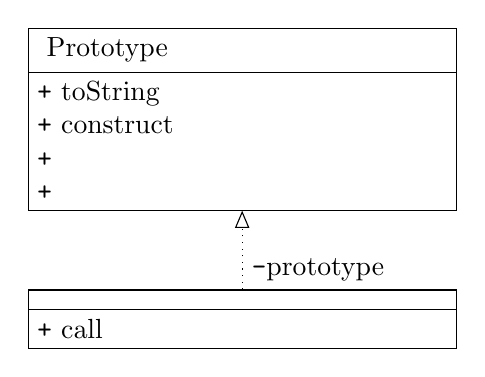
\begin{tikzpicture}
  \node (proto) [rectangle split, rectangle split part align=left, rectangle split parts=2,
      draw, text width=5.2cm] {
      \FlowLabel\ Prototype
  \nodepart{second}
      \texttt{+} \bracketdbl{toString}\\
      \texttt{+} \bracketdbl{construct}\\
      \texttt{+} \mjoin\\
      \texttt{+} \msubsumes
  };

  \node (obj) [below=1cm of proto.south, anchor=north,
      rectangle split, rectangle split part align=left, rectangle split parts=2,
      draw, text width=5.2cm]
  {
      \FlowLabelObject
  \nodepart{second}
      \texttt{+} \bracketdbl{call}
  };

  \draw[-open triangle 45, style=dotted] (obj.north) -- node[near start,right] {\texttt{-}\bracketdbl{prototype}} (proto.south);

\end{tikzpicture}
  \caption{UML class diagram of the first-class labeling system that introduces the \FlowLabel\ prototype constructor, and \FlowLabelObject\ instances.
  As in the ECMA~\cite{ecma} language standard, \bracketdbl{\textbullet} indicates implementation internal methods.}
  \label{fig:uml}
\end{figure}

The first-class labeling system also introduces a singleton \FlowLabel\ prototype that both holds methods common to all \FlowLabelObject\ instances and provides an interface through which the JavaScript developer can construct \FlowLabelObject s.
These first-class objects wrap the security labels propagated by \JitFlow\ and provide the developer an interface for label composition and application.
\autoref{fig:uml} uses UML to depict the relationship between the \FlowLabel\ prototype singleton and \FlowLabelObject\ instances.

\subsection{JavaScript Syntax Extension to Retrieve Labels}

The first-class labeling system implements a small change to the JavaScript language permitting JavaScript code to retrieve a label from a given value.
It introduces the keyword \mlabelof, as a new case in the \UnaryExpression\ grammar rule of the ECMA~\cite{ecma} language standard.
\autoref{fig:labelof} presents the entire grammar rule, including boldface emphasis on the new language keyword.

\begin{figure}[ht]
  \centering
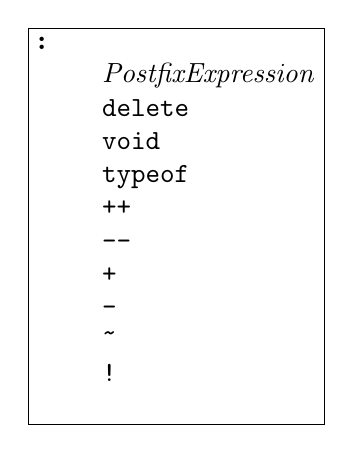
\begin{tikzpicture}
  \node (syntax) [anchor=south east, draw, align=left] {
    \UnaryExpression\textbf{:}\\
    $\hspace{2em}$ \textit{PostfixExpression}\\
    $\hspace{2em}$ \texttt{delete} \UnaryExpression\\
    $\hspace{2em}$ \texttt{void} \UnaryExpression\\
    $\hspace{2em}$ \texttt{typeof} \UnaryExpression\\
    $\hspace{2em}$ \texttt{++} \UnaryExpression\\
    $\hspace{2em}$ \texttt{--} \UnaryExpression\\
    $\hspace{2em}$ \texttt{+} \UnaryExpression\\
    $\hspace{2em}$ \texttt{-} \UnaryExpression\\
    $\hspace{2em}$ \texttt{\textasciitilde} \UnaryExpression\\
    $\hspace{2em}$ \texttt{!} \UnaryExpression\\
    $\hspace{2em}$ \textbf{\mlabelof\ \UnaryExpression}
  };

\end{tikzpicture}
  \caption{Modified JavaScript grammar rule for \UnaryExpression, highlighting the introduction of the \mlabelof\ keyword.}
  \label{fig:labelof}
\end{figure}
\vspace*{-\baselineskip}

\subsection{Network Hook in the Web Browser}

To permit the enforcement of policies written in JavaScript, the browser-hosted JavaScript environment includes one additional change.
Within WebKit, all network traffic conveniently passes through a single network interface class.
A network monitor interface wraps this class and reveals in through a function, \code{registerSendMonitor(fn)}, on the hosted \code{navigator} object.
Using this feature, the web developer can phrase application specific security policies concerning allowed network communication as a JavaScript function within the web application itself.
Once registered, these functions act as network monitors that inspect the payload of all resource requests before being sent over the network.

\section{Using First-Class Labels}
\label{sec:using-first-class-labels}

We design the first-class labeling system and its JavaScript API according to the functional programming paradigm, with the purpose of making it easier for web developers to adopt.
The first-class labeling API contains one minor syntax change to the JavaScript grammar, introducing the new \mlabelof\ operator and keyword.
It also extends the hosted environment (\emph{not} the ECMA specification) with a new built-in \FlowLabel\ prototype constructor object that holds methods for label composition (\mjoin) and comparison (\msubsumes).
Labels take the form of native built-in \FlowLabelObject\ instances, and behave with the same semantics as any other JavaScript object.
\JitFlow's first-class labeling features make a minimal set of changes necessary to expose its internal information flow framework.

The examples in this chapter show how the labeling framework detects and prevents information leakage that might occur due to a script injection attack.
All of the following examples show output of the labeling system at the JavaScript console.
Statements input to the console begin with a `\verb|>|'.
The console describes the resulting value in two parts: the value itself and the label attached to that value.

\subsection{Label Creation}

The first-class labeling extension of \JitFlow\ introduces a \FlowLabel\ prototype singleton to the JavaScript environment hosted by the web browser.
This object implements the internal \bracketdbl{construct} method so that JavaScript code may create first-class label objects.
The web developer may choose any valid JavaScript value to act as a security principal, and pass that value into the constructor.
After interning the provided value in the underlying framework's \FlowLabelRegistry, the constructor returns a \FlowLabelObject\ instance.
In the interest of avoiding attacks on the labeling system itself, \JitFlow's first-class labeling API does not provide programmatic access to the \FlowLabelRegistry.


\lstset{
  caption={Creating a Label Object.},
  label={list:create-label}
}
\begin{jscode}
> pwdLabel = new FlowLabel("pwd");
  [FlowLabelObject pwd] [FlowLabel example.com]
\end{jscode}

\autoref{list:create-label} shows a web developer creating a label using the JavaScript string, \codestringdbl{pwd}, as a security principal.
The web browser hosting \JitFlow\ automatically applies a label to every resource representing its domain of origin.
Consequently, the resulting \FlowLabelObject\ instance returned from the constructor itself carries a label representing the origin of this code snippet: \code{\url{example.com}}.

\subsection{Label Identification}

When the program uses a JavaScript value as a principal in the constructor of a \FlowLabelObject\, \JitFlow\ interns that value in the \FlowLabelRegistry.
Interning the principals allows fast unique identification of labels held by \FlowLabelObject\ instances.

\lstset{
  caption={Label Identity Operator.},
  label={list:identity}
}
\begin{jscode}
> lab1 = new FlowLabel("password");
  [FlowLabelObject password] [FlowLabel example.com]
> lab2 = new FlowLabel("pass" + "word");
  [FlowLabelObject password] [FlowLabel example.com]
> lab1 === lab2
  true [FlowLabel example.com]
\end{jscode}


\autoref{list:identity} shows that \JitFlow\ considers identical two different \FlowLabelObject\ instances constructed with equivalent string values.
As part of the interning process for the second label, \code{lab2}, the \FlowLabelRegistry\ first checks to see if the string argument, \code{"pass" + "word"}, has already been stored.
In this case, the first label, \code{lab1}, has already registered the same value.
The \FlowLabelRegistry\ responds by returning a \FlowLabelObject\ with the same underlying bit vector.
Line~\code{5} performs a comparison of the bit vector label values held by \code{lab1} and \code{lab2}, discovering the strict equality.

\subsection{Label Application}

The \FlowLabelObject\ instance acts as a first-class wrapper object around an internal bit-vector representation of a security label.
The \FlowLabelObject\ instance also implements the internal \bracketdbl{call} method, so that the security label may be attached to other JavaScript values.
When the \FlowLabelObject\ functor receives a passed value, it unions that value's current label with its internally stored label and returns the result.

\lstset{
  caption={Applying a Label to a JavaScript Value.},
  label={list:apply-label},
}
\begin{jscode}
> pwdLabel = new FlowLabel("pwd");
  [FlowLabelObject pwd] [FlowLabel example.com]
> pass = "24sk09nk12";
  24sk09nk12 [FlowLabel example.com]
> pass = pwdLabel(pass);
  24sk09nk12 [FlowLabel pwd, example.com]
\end{jscode}

\autoref{list:apply-label} shows the JavaScript developer applying the password label constructed previously (\autoref{list:create-label}), \code{pwdLabel}, to a string, \code{pass}.
After label application, the resulting password string carries a label describing both the domain of origin, \code{\url{example.com}}, and the password security principal, \codestringdbl{pwd}.

\subsection{Label Composition}

Behind each \FlowLabelObject\ lies a bit vector representation of a set of principals that describe the label's position in the lattice over principals held by the \FlowLabelRegistry.
The joining of two labels produces a new label that holds the principal set union of its arguments.
\JitFlow\ implements the join operation as an bitwise-or to maintain runtime performance.

\lstset{
  caption={Symmetry of Label Join.},
  label={list:label-join},
}
\begin{jscode}
> lab1 = new FlowLabel("label1")
  [FlowLabelObject label1] [FlowLabel example.com]
> lab2 = new FlowLabel("label2")
  [FlowLabelObject label2] [FlowLabel example.com]
> lab1.join(lab2)
  [FlowLabelObject label1, label2] [FlowLabel example.com]
> lab1.join(lab2) === lab2.join(lab1)
  true [FlowLabel example.com]
\end{jscode}

\autoref{list:label-join} illustrates the programmer composing a new label from two existing labels (Line~\code{5}).
\JitFlow\ makes this functionality readily accessible by supporting an \mjoin\ method on the built-in \FlowLabel\ prototype object.
As shown by the strict equality comparison (Line~\code{7}), the join operation is symmetric.

\subsection{Label Comparison}

In conformance with the lattice definition of subsumption, a label $A$ sumsumes another label $B$, written \code{A.subsumes(B)}, if and only if all of the principals within the second label $B$ also exist within the first label $A$.

\lstset{
  caption={Properties of Label \msubsumes\ Method.},
  label={list:label-subsumes},
}
\begin{jscode}
> lab1 = new FlowLabel("label1")
  [FlowLabelObject label1] [FlowLabel example.com]
> lab2 = new FlowLabel("label2")
  [FlowLabelObject label2] [FlowLabel example.com]
> lab3 = new FlowLabel("label3")
  [FlowLabelObject label3] [FlowLabel example.com]

> lab1.subsumes(lab1)
  true [FlowLabel example.com]

> (lab1.join(lab2)).subsumes(lab2)
  true [FlowLabel example.com]
> (lab1).subsumes(lab1.join(lab2))
  false [FlowLabel example.com]

> (lab1.join(lab2)).subsumes(lab1.join(lab3))
  false [FlowLabel example.com]
\end{jscode}

As shown in \autoref{list:label-subsumes}, all labels subsume themselves (Line~\code{8}).
Labels higher up the lattice only subsume lower ones when it contains all of the lower label's principals (Line~\code{11}), while lower labels can never meet this condition with respect to higher labels (Line~\code{13}).
Finally, labels on the same level of the lattice do not subsume one another (Line~\code{16}).

\subsection{Label Retrieval}

Not only can JavaScript programmers create label objects and apply them to program values, but they can also retrieve a first-class \FlowLabelObject\ from any tagged value.
\JitFlow\ provides the \mlabelof\ operator to accomplish this task.

\lstset{
  caption={Retrieving a Label from a Tagged Value.},
  label={list:label-labelof},
}
\begin{jscode}
> labA = new FlowLabel("labelA")
  [FlowLabelObject labelA] [FlowLabel example.com]
> x = labA("hello")
  hello [FlowLabel labelA, example.com]

> labB = new FlowLabel("labelB")
  [FlowLabelObject labelB] [FlowLabel example.com]
> x = labB(x)
  hello [FlowLabel labelA, labelB, example.com]

> labelof x
  [FlowLabelObject lableA, labelB, example.com]
    [FlowLabel labeA, labeB, example.com]

> (labelof x)("world")
  world [FlowLabel labelA, labelB, example.com]

> (labelof x) === labA.join(labB)
  true [FlowLabel labelA, labelB, example.com]
\end{jscode}

\autoref{list:label-labelof} shows an example usage of the \mlabelof\ operator to retrieve a first-class \FlowLabelObject\ from a program value (Line~\code{11}).
The programmer can then use the resulting \FlowLabelObject\ to apply a label to other values (Line~\code{15)} or tested as part of a label comparison (Line~\code{18}).

\subsection{Authoring a Network Monitor}
\label{subsec:network-monitor}

We now assume that the attacker injects code using \code{sniffPassword} (\autoref{list:sniffPassword}) in an attempt to drop the label of the user's password.
Because \JitFlow\ tracks labels inter- and intra-procedurally with respect to both data and active implicit control flows (\autoref{ch:terminology}), the label on the resulting sniffed password carries both the attacker's principal and the user's password principal.
The first-class labeling system exposes the network object to JavaScript, allowing interception of the information leak at the time of a network request.

\lstset{
  caption={Developer Provided Network Monitor Function.},
  label={list:network-policy},
  firstnumber=1,
}
\begin{jscode}
navigator.registerSendMonitor(
  function(method, url, payload) {
    if (method == 'GET') {
      var lab = new FlowLabel("example.com");
      lab = lab.join(new FlowLabel("pwd"));

      if (!lab.subsumes(labelof url))
        log(url + " has unexpected label");
      if (!lab.subsumes(labelof payload))
        log(payload + " has unexpected label");
    }
    // other types of network request elided
    return true;
  });
\end{jscode}

Suspecting a possible information leak, the web developer implements a network monitoring logic in a JavaScript method, and registers it through the newly exposed API method, \code{navigator.registerSendMonitor}.
When the attack code attempts to communicate the pilfered information over the network, the web browser first executes all registered monitors (in registration order) to determine if the request conforms to the developer-specified policy function.

\autoref{list:network-policy} shows an example network monitor that takes advantage of the labels automatically applied by the browser.
On Line~\code{4}, the developer creates a label representing the security principal, \code{\url{example.com}}.
The \FlowLabelRegistry's interning of principals ensures that any labels created in this monitor function exactly match the same labels created elsewhere.

Through prototype-based inheritance, all \FlowLabelObject\ instances have a \mjoin\ method that returns a new \FlowLabelObject\ instance representing the union of its argument \FlowLabelObject\ instances.
On Line~\code{5} of \autoref{list:network-policy}, the developer \mjoin s the security principal \code{\url{example.com}} with \codestringdbl{pwd} to compose together existing labels into a single label representing the union of all principals the developer wishes to allow in an HTTP GET request.

Information flow propagation within the \JitFlow\ VM labels each new value with the join of the labels of the arguments used to construct that value.
Consequently, label propagation naturally results in values labeled with more than one principal, even when the original program only seeded a few values, each with a single principal.
In response to this phenomenon, our developer uses the \msubsumes\ method (Line~\code{7} and Line~\code{9} of \autoref{list:network-policy}) to check that the label of the request is a subset of all allowed principals.

Although the first-class label wrappers also permit strict equality comparison (JavaScript operator \code{===}) between two \FlowLabelObject\ instances, we strongly encourage using the \msubsumes\ relation for expressing security policy constraints using subsets of principals.
This practice allows catching all values with labels below the given upper bound (supremum).

\JitFlow's labeling extension introduces the \mlabelof\ operator so that JavaScript code can retrieve labels attached to variables for inspection and application.
On Line~\code{7} and Line~\code{9} of \autoref{list:network-policy}, the developer uses this operator to obtain the label attached to the target request \code{url}, and network \code{payload}.
Because \JitFlow\ propagates labels following data flows, the resulting \FlowLabelObject\ instance returned from \mlabelof\ operator itself carries a label containing the union of the provided argument and current program counter.
If desired, the developer may use the resulting \FlowLabelObject\ instance to label other values.

In the example shown in \autoref{list:network-policy}, the developer constructs a label over the password principal, \codestringdbl{pwd}, at two different code locations: once to label the user's input and again in the network monitor.
This practice causes no problem for the labeling system, because the \FlowLabelRegistry\ interns principals, allowing our system to consider identical, two \FlowLabelObject\ instances constructed in different code locations but with equivalent JavaScript values.

\section{Evaluation}
\label{sec:first-class-evaluation}

To evaluate the effectiveness of \JitFlow's first-class labeling system for security debugging we examine four dimensions:
\begin{description}
\item[Performance.] We show that underlying information flow framework remains fast compared to other work and argue that the first-class labeling system introduces negligible overhead.
\item[Completeness.] The first-class labeling system inherits the code coverage of the supporting information flow framework.
\item[Security.] We argue that the labeling system revealed to the JavaScript programmer does not present a new attack surface in any significant way.
\item[Usability.] We demonstrate how developers can use the system to debug security vulnerabilities in their web applications.
\end{description}

We evaluate the effectiveness of \JitFlow's role as a security debugging tool for web applications.
We measure the robustness and performance of the underlying labeling framework, demonstrating that even sites with large libraries of JavaScript code present no execution difficulties.
We also use the first-class labeling system to find and debug an XSS vulnerability.

\subsection{Performance}
\label{sec:first-class-performance}

\JitFlow, modifies WebKit's JavaScript engine JavaScriptCore (version~1.4.2) to attach labels to every value.
Additionally, it contains a lattice data structure relevant for mapping bits within a label to security principals (the \FlowLabelRegistry), which the hosting web browser uses for mapping label bits to domains.
\JitFlow\ also modifies the internal \JSValue\ representation to attach labels to program values, and a control flow stack that assists in propagating active implicit information flow dependencies at runtime.
To evaluate the costs imposed by \JitFlow's labeling and tracking implementation, we test it against an unmodified JavaScriptCore of the same version.

For an apples-to-apples comparison, we execute both \JitFlow\ and the unmodified JavaScriptCore with just-in-time compilation disabled.
A dual Quad Core Intel Xeon~2.80~GHz with 9.8~GiB RAM running Ubuntu~11.10 executes all benchmarks (at niceness level -20).
We chose to use the SunSpider~\cite{sunspider} benchmark suite because its status as the standard benchmark suite for JavaScript makes it suitable for comparisons to other work.
SunSpider includes test cases that cover common web practices, such as encryption and text manipulation, but does not include any first-class labeling operations.
This benchmark test provides a measure of the baseline overhead involved in maintaining information flow data structures and propagating labels.

\begin{figure}[ht]
  \centering
  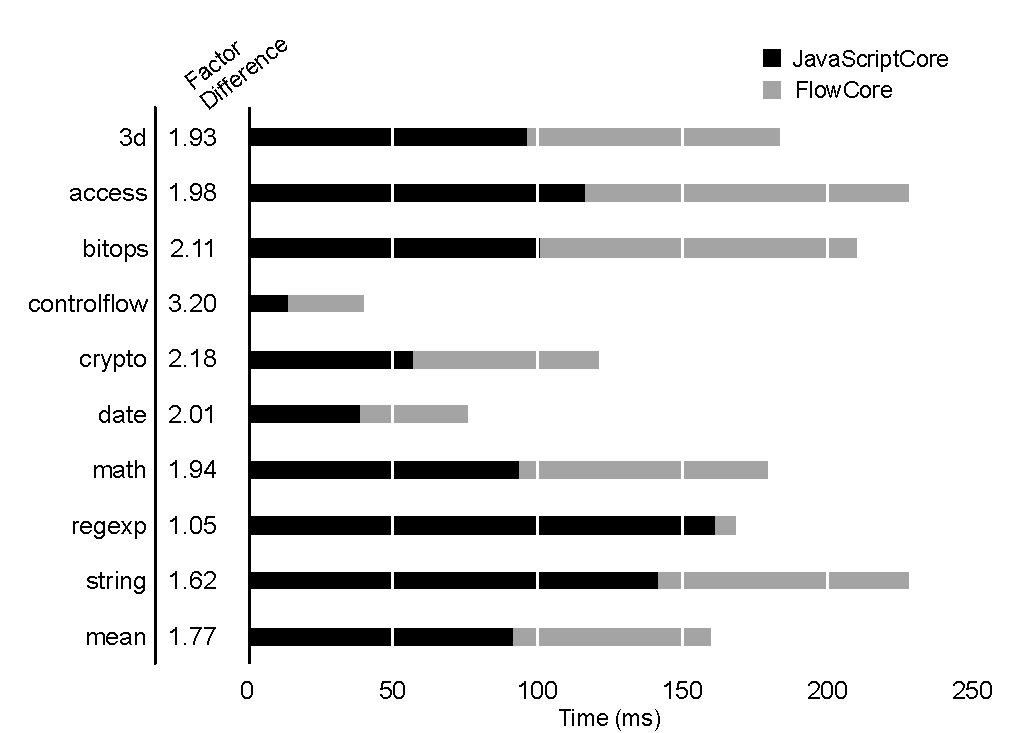
\includegraphics[width=\textwidth,keepaspectratio=true]{graphics/sunspider-jsc-vs-flowcore.pdf}
  \caption{SunSpider Benchmark results (interpreters only): JavaScriptCore vs. \JitFlow.}
  \label{fig:first-class-sunspider}
\end{figure}

\autoref{fig:first-class-sunspider} reveals overall execution speed of JavaScript benchmark results: \JitFlow\ has a mean execution time of 158.33~ms, whereas JavaScriptCore has a mean execution time 89.44~ms.
The SunSpider benchmark does not contain first-class labeling operations, so the overall 77\% slowdown represents the overhead incurred by \JitFlow's implementation of label propagation.
In comparison, other information flow approaches~\cite{just.etal+11} introduce a 150\% slowdown making programs two to three times slower.

%\JitFlow\ extends all values within the VM by 64 bits so that both JavaScript primitives and object references carry a label.
The bit vector representation permits \JitFlow\ to carry out label propagation via bitwise-or.
By packing the label into the \jsvalue (\autoref{sec:jitflow-labelencoding}), \JitFlow\ ensures that a full first-class label object exists only when explicitly constructed (\code{new} \FlowLabel) or retrieved (\mlabelof) by the developer.
As a result, the introduction of the first-class labeling system into the hosted environment incurs no additional runtime performance overhead compared to a fully automatic labeling system.
We do not evaluate the performance impact of evaluating functions attached to the network hook, because it remains insignificant within a debugging environment and the developer has the power to implement any monitor function they desire.
However, evaluating the monitor function will add overhead to all network requests.

The performance of the underlying labeling framework implies that even sites with large amounts of JavaScript code execute without noticeable slowdown.
To test whether the information flow tracking framework causes a noticeable performance decrease, we used \JitFlow\ to visit (and log into) JavaScript intensive sites, such as Facebook, GMail, Google Maps, Bing, GitHub and Cloud9 IDE.
These sites do not make use of the first-class labeling system introduced in this paper.
However, user interaction proves that the performance overhead of the labeling framework does not introduce any usability issues.

\subsection{Completeness}

To verify that the underlying framework does not introduce any runtime bugs when interpreting either machine-generated or human-written JavaScript found in the wild, we scripted the web browser hosting \JitFlow\ to automate the visiting of all sites in the Alex Top 500~\cite{alexa}.
This webcrawler injects code into each page, to perform two actions: (1) attach a network monitor and (2) fill out and submit the first form on the page using data labeled with an identifying principal.
The injected monitor verifies that the submitted form generates a request containing the identifying principal.
The automated crawl checks that \JitFlow's label propagation engine can execute JavaScript code in the wild.

The first-class labeling system also aided development of \JitFlow\ itself.
For each of the data-flow and control-flow features covered by the tracking engine (\autoref{ch:label-tracking}), we created a unittest case that ensures the semantic correctness of the applied labels.
The ability to apply labels to specific values, pass them through computation, and then verify that the attached labels upgrade accordingly proved exceedingly useful throughout the \JitFlow's development cycle.
Without first-class labels to assist in writing a unittest suite, we would feel far less confident of the \JitFlow's labeling capabilities.

\subsection{Security}

The labeling framework \JitFlow, generates, at runtime, new security principals for every unique label generated by the developer and new domain encountered by the web browser.
Introduction of runtime principals requires mutation of the \FlowLabelRegistry.
By design, \JitFlow\ does not support declassification, preventing a communication channel via the labeling framework itself.

\JitFlow's first-class labeling system exposes, to the web application and any injected code, a JavaScript API for creating and applying labels to JavaScript values.
This exposure represents a new attack surface that might allow an attacker to target the labeling framework itself.
However, we envision web developers using the first-class labeling system only in a testing environment, where it provides no benefit to the attacker.
Nevertheless, even when used by all clients, the lack of declassification means that the attacker-injected code cannot drop labels applied by the developer for debugging purposes.

Finally, the browser component allows registration of many monitor functions, through a JavaScript interface accessible by code injected into the web application.
It evaluates all monitor functions registered, in registration order.
The developer-supplied monitor function executes for as long as all previous monitors in the chain return \code{true}, indicating an allowable flow.
So, in the worst case, an attacker can register their own monitor function first, preempting the execution of the developer's monitor.
But this injection only allows the attacker to halt the chain by returning \code{false}, indicating a policy-violating flow.
Semantically, the system only considers an information flow allowable when \emph{all} monitors in the chain indicate success by returning \code{true}.

\subsection{Utility as a Debugging Tool}

To evaluate the first-class labeling system as a tool for testing web applications and discovering security vulnerabilities, we create a web page that contains a user login form.
Acting as a malicious developer, we insert code into the page, which uses the \code{sniffPassword} label dropping code (\autoref{list:sniffPassword}) prior to exfiltrating the form contents to a second server via both an \code{XmlHttpRequest} and as part of an \code{img.src} URL.
Acting as a security researcher, we mirror the page and add labeling code that applies a tag to the form's DOM node and a network monitor function that checks for the unique tag.
Visiting the mirrored page successfully triggers the monitor function, alerting us to the exfiltration.
WebKit's developer tools assisted with finding the portion of the page responsible for generating the image request.

For a more realistic example, we attempt a similar attack using a mirrored \url{ebay.com} page obtained from XSSed~\cite{xssed}, this time targeting the site's cookie.
This page loads content from several different sources, and contains an XSS vulnerability that we exploit to inject the exfiltration code.
Because the browser hosting \JitFlow\ automatically labels the cookie with the domain of origin, we did not need to insert labeling code.
Instead, we find it sufficient to implement a network monitor that checks only whether data sent to an origin does not contain third-party principals.
This monitor detected the exfiltration of the cookie (labeled with \url{ebay.com}) being sent to a server other than \url{ebay.com}.
Again, WebKit's developer tools assisted with pinpointing the JavaScript code responsible for the request.

%========================================================================

\section{Summary}
\label{sec:first-class-summar}

\JitFlow\ presents to the JavaScript developer a first-class labeling system that exposes an underlying information flow framework.
Developers can use their domain knowledge to label JavaScript values within their application and construct network monitor policies that selectively ignore automatically applied labels.
The labeling system provides dynamic creation of security principals, supporting the common practice of loading code and resources from many different domains in web applications.

\JitFlow\ introduces a new built-in \FlowLabelObject\ class to the hosted environment, which the developer uses to selectively label JavaScript values.
The developer creates \FlowLabelObject\ instances using existing JavaScript values as security principals or by composition with other \FlowLabelObject\ instances via the lattice \join\ method.
The \msubsumes\ method allows comparison of all \FlowLabelObject\ instances reporting their subset relation within the label lattice, while the strict equality operator (\code{===}) allows unique identification of labels by their internal bit vector representation.
Together with the ability to retrieve labels attached to values via the new built-in \mlabelof\ operator, \JitFlow\ gives the developer the means to implement security policies in JavaScript.

Because of the shared underlying data-structures, exposing the labeling framework as first-class language objects to the developer incurs no additional runtime cost compared to automatic labeling systems.
It allows developers to leverage their domain knowledge and existing JavaScript experience and direct their focus on identifying and debugging application specific information flows.
For sites that have large amounts of JavaScript code, the system can be used in a testing environment.
First-class labels allow developers to improve the security of their applications by writing policies in JavaScript that selectively ignore the high quantity of reports produced by automatically attached labels.

%========================================================================
\begin{comment}
\section{Tracking JavaScript Information Flows}

% Previous work~\cite{empirical-study} identifies history sniffing as the primary use of active implicit flows.

Label propagation within the JavaScript VM occurs at the construction of every temporary value.
As shown in \autoref{list:indirect-flows-functions}, it can track, at runtime, labels across multiple assignment statements and function calls.
The example shows that temporary computed values (those not assigned to a variable) also carry a label.
And that labels are propagated into, through, and from function calls.

\begin{lstlisting}[caption={Example Indirect Explicit Flows in Functions},label={list:indirect-flows-functions}]
> labelGood = new FlowLabel("good");

> function echoArgs(arg) {
>    print(labelof arg);
>    return arg;
> }
> echoArgs(labelGood(7));
  [FlowLabelObject good] // print arg
   7 [FlowLabel good]
  
> function applyLabel(arg) {
>    var labelBad = new FlowLabel("bad");
>    return labelBad(arg);
> }
> applyLabel(7)
  7 [FlowLabel bad]

> labelFoo = new FlowLabel("foo")
> labeledFunction = labelFoo(echoArgs);
> labeledFunction(7);
  [FlowLabelObject ] // print arg
  7 [FlowLabel foo]

\end{lstlisting}
\end{comment}

\begin{comment}
\subsection{Indirect Explicit Flows in Arrays}

We also handle some special fields, such as Array.length, and other operations, such as indexing (also on strings).

\begin{lstlisting}[caption{Example Indirect Explicit Flows in Array Objects},label={list:indirect-flows-arrays}]
> labelGood = new FlowLabel("good.com")
> myArray = labelGood([10,11,12,13,14]);

> myArray.length
  [TODO]

> myArray[3]
  13 [FlowLabel good]

> myArray[100]
  undefined [FlowLabel good]
\end{lstlisting}
\end{comment}

\begin{comment}
\subsection{Active Implicit Flows}

An example of such an implicit flow can be seen in the password sniffing code in \autoref{list:implicit-flow}.
Both the stopping condition of the loop, and the argument to the switch statement label the program counter with \textsf{good.com}.
Inside the switch, all assignments also carry the program counter label.

\begin{lstlisting}[caption={Example Indirect Explicit Flow},label={list:implicit-flow}]
> labelGood = new FlowLabel("good.com")
> password = labelGood("o24sk09nk12")

> function sniffPassword(pw) {
>     spw = "";
>     for (var i = 0; i < pw.length; i++) {
>         switch(pw[i]) {
>         case 'a':
>            spw += 'a';
>         case 'b':
>            spw += 'b';
>         ... // other characters elided
>         }
>    }
>    return spw;
> }

> sniffPassword(password);
  42 [FlowLabel good.com]
\end{lstlisting}

\end{comment}

\begin{comment}
\subsection{Property Hijacking Attack}

\todo{this example doesn't really motivate first-class labels. How to change it? write checks around uses?}
As documented by Chess et al.~\cite{js-hijacking} it is possible for attackers to hijack the getter and setter functions on native object prototypes such as \textsf{Object} and \textsf{Array}.
For example, in \autoref{list:prototype-hijacking} the attacker modifies \textsf{Object.prototype} such that it will run the \textsf{stealPassword} function whenever any object's \textsf{password} field is updated.
A real attack would have \textsf{stealPassword} communicate its argument back to an attacker controlled server, via a network request.
Because attacker supplied code is used to perform the hijacking, our labeling system causes the \textsf{\_\_password} field to carry the attacker's label.

\begin{lstlisting}[caption={Example Prototype Hijacking Attack},label={list:prototype-hijacking}]
Object.prototype.__defineSetter__("password",
  function(x) {
    stealPassword(x);
    this.__password = x;
  })

Object.prototype.__defineGetter__("password",
  function() {
    return this.__password;
  })
\end{lstlisting}


\begin{figure*}[ht]
  \centerline{\includegraphics[width=18cm,keepaspectratio=true]{graphics/example.pdf}}
  \caption{write text here.}
  \label{fig:example}
\end{figure*}

\end{comment}

\begin{comment}
\subsection{Monitoring the Flow}

\todo{how often is it the case that a secret was involved in early control flow. example: password-based login determines whether app gets run. A successful login taints app execution.}

** Example
  1. taint a pin, and have network traffic: can detect when it gets passed through the network
     (no) at each ajax request, developer can add a if-else label detection check
     (yes) at each request, browser uses config file to check them all (ship policy in the head, ref related work)
  2. malicious script tries to grab value directly
  3. malicious script tries to grab value through indirect flow

  - developer knows their framework, and can label the form fields where user enters sensitive data
  - can also happen via js plugins (greasemonkey) 

  : shim form entry, catch that users don't input pin in email or other field, via regex/js labeler
\end{comment}

\begin{comment}
*** Weaknesses
  - developer might forget to label a sensitive value
  - developer has to put in the checks, what if they forget one? [browser shim network]
    - if they have to put in the checks, what if attacker includes an ajax request? does it get around the checks?
  - site could shim the request object, but they'd have to get there first (before attacker);
  - could check all network traffic, and report all labels (developer can filter out what they want)

  - might be lots of work for developer
    : but can have default whitelist/self-domain policy, the network monitor optional
\end{comment}

\begin{comment}
\subsection{Security Analysis}

%*** Demonstrate tagging and inspecting values
%    Example of something first class labels can do that couldn't be done before
%    : done in example
%*** Performance (Sunspider, v8, craken, and (not honest) Dromaeo)
%    - need complete vs selective labeling
%*** What can first class labels do that other Systems can't?
%    - programmer can specify which values to track
%    nice to get list of all affected variables?
%*** Demonstrate lower false positive rate
%    - shim the network traffic to label some objects on large site (facebook)
%*** Measure the number of useful vs nop label operations
%    => quantifies argument for sparse labeling
%       and vm-level optimizations
%*** Prevent leak of tainted data in a custom mashup!
%
%3 dimensions (plot triangle)
%- perf
%- security
%- developer effort 

\end{comment}



\chapter{Just-In-Time Compilation}
\label{ch:jitflow}

\newcommand{\codeline}[1]{line~\code{#1}}
\newcommand{\Codeline}[1]{Line~\code{#1}}
\newcommand{\codelines}[2]{lines~\code{#1}--\code{#2}}
\newcommand{\bcodeline}[1]{offset~\code{#1}}

\newcommand{\jsvalue}[0]{\code{JSValue}}
\newcommand{\jsvalues}[0]{\code{JSValue}s}

Experience integrating \FlowCore\ with the WebKit browser and visiting pages in the Alexa Top 1,000~\cite{alexa} revealed important issues about JavaScript's omnipresence on the Web.
In particular, that effort discovered that today's highly-interactive web applications rely on a performant JavaScript interpreter backed up by a just-in-time compiler.

Several recent approaches~\cite{vogt.etal+07,just.etal+11,groef.etal+12,kerschbaumer.etal+13} have shown that information flow tracking mitigates the shortcomings of current web security practices and successfully counters XSS-based information theft attacks.
Even though these dynamic tracking enhancements provide the desired security, all of the previous approaches suffer from the drawback of incurring performance penalties of at least 80\%.
Furthermore, they all integrate the tracking logic in the JavaScript interpreter, which itself commonly performs around four times worse than code generated by a just-in-time (JIT) compiler (\autoref{sec:jitflow-evaluation-performance}).

Currently, browser vendors compete for adoption by advertising JavaScript performance.
As a result of the ``browser wars,'' faster JavaScript virtual machines (VMs) now enable web applications with large amounts of JavaScript code.
Consequently, the slowdown seen when integrating information flow into the JavaScript interpreter represents a major obstacle to adoption.

The project that started \FlowCore\ answers this challenge by implementing dynamic information flow tracking in a JIT compiler.
The updated engine, \JitFlow, allows detection of suspicious network traffic that sends data to a server other than that intended by the application programmer.
The detection occurs at runtime, catching the code ``in flagranti'' when performing malicious actions such as data theft.

The work behind \JitFlow\ contributes:

\begin{itemize}

\item The first (to the best of my knowledge) dynamic information flow tracking engine in a JIT compiler for a dynamically typed programming language.

\item Several optimizations (\autoref{sec:jitflow-implementation}) essential to preserving the performance gains when JIT compiling the information flow tracking logic.

\end{itemize}

\section{The Threat of executing third Party Code}
\label{sec:jitflow-thirdpartycode}

The Same Origin Policy, still widely in use as a first line of defense in web applications, permits scripts access to methods and properties when sharing the same origin and restricts access otherwise.
Unfortunately, rules of the Same Origin Policy often clash with modern web application architecture, because the SOP only applies to cross-frame communication.
Previous experience with CrowdFlow~\cite{kerschbaumer.etal+13} shows that, within the Alexa top 500, some pages contain information influenced by code originating from up to six different domains is sent across domain boundaries.
Verification and proof that the mashup performs only the expected task and does not steal data is not available.
Hijacking just one commonly included script compromises the privacy of many web users~\cite{nikiforakis.etal+12}.

%------------------------------------------------------------------------------------------------------
\subsection{The Nature of Code Injection Attacks}
\label{sec:jitflow-codeinjection}

Because servers deliver JavaScript as source text, most content and third-party library providers compact their code by automatically shortening variable names, removing all extra whitespace as well as line breaks so the code becomes as small as possible.
This practice shortens the transfer time for loading JavaScript, but has the side effect of obfuscating the source code.
Web authors are unlikely to audit compressed code for security holes despite the fact that including it in the same execution context as the web application grants it access to application internals.
Consequently, a channel through which attackers can inject code that steals sensitive user information remains open and prevalent.

In addition to the risk of including such malicious third party code, I'd like to remind the reader of two other forms of code injection attacks.
Based on the method of injection, I distinguish between:

\begin{itemize}

\item \textit{Non-Persistent (Reflected) attacks}, that occur when the server sends client-provided code embedded in HTTP query parameters and HTML form submissions back to the user as page content after processing by the web application servers.

\item \textit{Persistent attacks}, that occur when the web application stores client-provided data server-side and reflects it back to subsequent visitors.

\end{itemize}
In both of these cases, from the client's perspective, the origin of the attacker code is the same as that of the web application itself, meaning that the Same Origin Policy can not prevent the attack.
Additional security requires a more powerful, behavior-focused mechanism, such as information flow tracking.

%------------------------------------------------------------------------------------------------------
\subsection{Threat Model}
\label{sec:jitflow-threatmodel}

As assumed when evaluating \FlowCore\ (\autoref{sec:first-class-evaluation}), I grant the attacker with the ability to inject code into a web application.
The attacker accomplishes injection by exploiting a XSS vulnerability or the ability to provide content for mashups, advertisements, libraries, etc. which other sites include.
To collect the stolen data, the attacker controls their own web host.
The attacker practices only code injection techniques and does not resort to packet sniffing, network interception, or control of the application servers.

%------------------------------------------------------------------------------------------------------
\subsection{Provided Security}
\label{sec:jitflow-providedsecurity}

The web browser running \JitFlow\ advanced significantly beyond the capabilities offered when evaluated with only the interpreter \FlowCore.
The updated browser protects against several information theft attacks, including, but not limited to:

\begin{itemize}[itemsep=4pt,parsep=4pt]

\item \textit{Sensitive Data Theft Attacks:}
By sending a GET request to a server under the attacker's control, the attacker can steal information in the URL of an image request:

\begin{snippet}
elem.src = "evil.com/pic.png?" + credit_card_number;
\end{snippet}

The attacker uses the request for the image as a channel to steal the user's credit card number as a payload in the GET request.
Merely changing the URL targeted by the \code{src} attribute of an image triggers loading of the image.

\item \textit{Keylogging Attacks:}
Similarly, to steal a username and password combination, an attacker might craft code that logs keystrokes by registering an event handler:

\begin{snippet}
document.onkeypress = listenerFunction;
\end{snippet}

The listener function records the user's keystrokes and sends them to the attacker's server through an HTTP request.

\item \textit{Cookie Stealing Attacks:}
Furthermore, if a script can access cookies, then an attacker can also steal a session cookie between the browser and an honest site by concatenating the \code{document.cookie} to the URL of the image request.
The stolen cookie allows the attacker to impersonate the user and hijack the user's session.

\end{itemize}

%------------------------------------------------------------------------------------------------------
\subsection{Sample Attack: Stealing Form Data}
\label{sec:jitflow-stealingformdata}

An HTML form provides a page with data entry fields that allow a user to enter text such as a username and password.
Once a user submits the form, the browser sends the data to the server.
Virtually all web applications rely on login fields to authenticate their users.
If an attacker manages to inject code into a web application that contains a login form, the attacker's script can read a user's credentials and send them to an attacker-controlled server.
Later, the attacker may use the stolen credentials to impersonate users of the web service.

\lstset{
  label=list:fieldinfo,
  caption={Example attack code that steals login form data from a web page.}
}
\begin{jscode}
// place hidden image on the page
var pixel = "<img src=\"http://www.attacker.com/pixel.png\"" +
            "id=\"pixel\" />";
document.write(pixel);

function stealFormData(type, value) {
  var payload = "url=" + document.domain + "&" + type + "=" + value;
  document.getElementById("pixel").src =
      "http://www.attacker.com/pixel.png?" + payload;
}

// add stealFormData to all forms on page
for (var i = 0; i < document.forms.length; i++) {
  for (var j = 0; j < document.forms[i].elements.length; j++) {
    var elem = document.forms[i].elements[j];
    elem.addEventListener("blur", // triggered when element loses focus
           function() { stealFormData(this.type, this.value) }, false);
  }
}
\end{jscode}

\autoref{list:fieldinfo} shows exploit code an attacker might use to steal credentials from the login form of a web page.
The attack script first loads an image (\codeline{2}) supplied by a server under the attacker's control.
The attacker designs the image to avoid perceptible changes in page layout.
Few users will notice the placement of a single transparent pixel, but the attacker can use the GET request as a channel to steal confidential page data whenever the image is reloaded from the server.

The attacker knows users will fill out the form and registers (\codelines{14}{15}) a \code{blur}-event handler on all forms elements on the page.
When a form element loses focus it triggers a call to the \code{blur}-event handler.
The handler, \code{stealFormData} defined on \codeline{5}, first encodes information about the page domain and contents of the form element which triggered the event in the \code{payload} variable.
Then it updates the \code{src} attribute of the image with a URL containing the payload.
This update causes the browser to automatically reload the image, sending the sensitive information in the URL of the image request.

\lstset{
  label={list:serverlogs},
  caption={Log of \code{attacker.com} from the running example.}
}
\begin{jscode}
[01/Jan/2014:21:34:10] "GET /pixel.png?url=www.bank.com&text=alice HTTP/1.1"
[01/Jan/2014:21:34:12] "GET /pixel.png?url=www.bank.com&password=bob69 HTTP/1.1"
\end{jscode}

By inspecting the server request logs, the attacker can reassemble the captured form data.
\autoref{list:serverlogs} contains some example entries of image requests.
The attacker can clearly identify a user of \code{www.bank.com} with login `\code{alice}' having the password `\code{bob69}'.

The webpage \textit{About The Open Web Application Security Project}~\cite{xsscheatsheet} hosts an extensive list of XSS vulnerabilities that provides a detailed description of all the different kinds of XSS attacks.

%xxxxxxxxxxxxxxxxxxxxxxxxxxxxxxxxxxxxxxxxxxxxxxxxxxxxxxxxxxxxxxxxxxxx

\section{Changes Made to the Information Flow Framework}
\label{sec:jitflow-framework}

Whether an interpreter or JIT-compiled code performs information flow tracking, the implementation requires supporting data structures and other modifications to the runtime VM.
\JitFlow\ makes some alterations to the underlying data structures that once supported \FlowCore.
Each modification focuses on increasing the performance of the tracking engine to support runtime compilation of code in \JitFlow.

\subsection{The Label Lattice}

Because \JitFlow\ forms the core of an information flow tracking web browser, it focuses on the ability to web map domains to security principals.
Previous experience~\cite{kerschbaumer.etal+12, kerschbaumer.etal+13} demonstrate that most web pages do not include more than 16 separate web origins.

\JitFlow\ retains the \FlowLabelRegistry, but reduces the number of bits used to represent a label.
The \FlowLabelRegistry\ still follows Myers' decentralized label model~\cite{myers.liskov+00} and represents security labels as a lattice join over domains (\autoref{fig:jitflow-label-lattice}).

\begin{figure}[ht]
 \centering
 \resizebox{\textwidth}{!}{
\begin{tikzpicture}[node distance = 1cm, auto,
    force/.style={rectangle, inner sep=5pt, text badly centered, minimum height=.8cm},
    every text node part/.style={align=center},
    ]

    \begin{scope}[yshift=4cm, xshift=-8cm]
    \node[shape=rectangle, draw] {
       \begin{tabular}{l|c}
          \multicolumn{2}{c}{\code{LabelRegistry} mapping} \\
          \hline
          \url{good.com} & \code{001} \\
          \url{other.com} & \code{010} \\
          \url{evil.com} & \code{100} \\
       \end{tabular}
    };
    \end{scope}

    \begin{scope}
    \matrix[nodes={force}, column sep=1cm, ampersand replacement=\&] {
        \node (ex) {\url{good.com} \\ \code{001}}; \&
        \node (mp) {\url{other.com} \\ \code{010}}; \&
        \node (ad) {\url{evil.com} \\ \code{100}}; \\
    };
    \end{scope}

    \begin{scope}[yshift=2cm]
    \matrix[nodes={force}, column sep=.5cm, ampersand replacement=\&] {
      \node (exUmp) {\url{good.com} $\sqcup$ \url{other.com} \\ \code{011}}; \&
      \node (exUad) {\url{good.com} $\sqcup$ \url{evil.com} \\ \code{101}}; \&
      \node (mpUad) {\url{other.com} $\sqcup$ \url{evil.com} \\ \code{110}}; \\
    };
    \end{scope}

    \begin{scope}[yshift=4cm]
    \matrix[nodes={force}, column sep=1cm] {
      \node (exUmpUad) {\url{good.com} $\sqcup$ \url{other.com} $\sqcup$ \url{evil.com} \\ \code{111}}; \\
    };
    \end{scope}

    \begin{scope}[yshift=-2cm]
    \matrix[nodes={force}, column sep=1cm] {
      \node (bot) {interpreter \\ {$\bot$}}; \\
    };
    \end{scope}

    \draw[arrow] (ex) -- (exUmp);
    \draw[arrow] (ex) -- (exUad);

    \draw[arrow] (mp) -- (exUmp);
    \draw[arrow] (mp) -- (mpUad);

    \draw[arrow] (ad) -- (exUad);
    \draw[arrow] (ad) -- (mpUad);

    \draw[arrow] (exUmp) -- (exUmpUad);
    \draw[arrow] (exUad) -- (exUmpUad);
    \draw[arrow] (mpUad) -- (exUmpUad);

    \draw[arrow] (bot) -- (ex);
    \draw[arrow] (bot) -- (mp);
    \draw[arrow] (bot) -- (ad);

\end{tikzpicture}
}
  \caption{Example Label Lattice for domains \url{good.com}, \url{other.com}, and \url{evil.com}}
  \label{fig:jitflow-label-lattice}
\end{figure}

It stores a mapping from web security principals (domain name strings) to unique bit positions.
Taken as a whole, these bit positions form a bit vector that acts as a confidentiality label, holding up to 16~different domains.

\subsection{Encoding Labels}
\label{sec:jitflow-labelencoding}


The \FlowCore\ interpreter, already achieves high performance by using a type-tagged union, called \jsvalue, to represent immediate values, object references, and numbers.
However, the fat value extension from 64-bit \jsvalues to 128-bit entities that join a value and label tag, proved itself too radical a change for the JavaScriptCore's JIT engine.
Fat values required updating offset calculations scattered throughout the code base.

\begin{figure}[ht]
  \centering
\begin{tabular}{cccc|l}
    \multicolumn{4}{c|}{bit values} & type  \\
\hline
    \code{0000} & \code{xxxx} & \code{pppp} & \code{ppp0} & \code{pointer} \\
\hline
    \code{0000} & \code{xxxx} & \code{0000} & \code{0000} & \code{empty} \\
    \code{0000} & \code{xxxx} & \code{0000} & \code{0002} & \code{null} \\
    \code{0000} & \code{xxxx} & \code{0000} & \code{0004} & \code{deleted} \\
    \code{0000} & \code{xxxx} & \code{0000} & \code{0006} & \code{false} \\
    \code{0000} & \code{xxxx} & \code{0000} & \code{0007} & \code{true} \\
    \code{0000} & \code{xxxx} & \code{0000} & \code{000a} & \code{undefined} \\
\hline
    \code{FFFF} & \code{xxxx} & \code{iiii} & \code{iiii} & \code{integer} \\
\hline
    \code{0001} & \code{dddd} & \code{dddd} & \code{dddd} & \tikzmark{2nd} \multirow{3}{*}{\code{  double}} \\
    \code{\vdots} & & & & \\
    \code{FFFE} & \code{dddd} & \code{dddd} & \code{dddd} & \tikzmark{4th} \\
\hline
     \tikzmark{p1}\code{~~~}\tikzmark{p2} & \tikzmark{p3}\code{~~~}\tikzmark{p4} & \tikzmark{p5}\code{~~~}\tikzmark{p6} & \multicolumn{1}{c}{\tikzmark{p7}\code{~~~}\tikzmark{p8}} & \multicolumn{1}{l}{\tikzmark{p9}} \\
     & & \tikzmark{v1}\code{~~~~} & \multicolumn{1}{c}{\code{~~~~}\tikzmark{v2}} & \multicolumn{1}{l}{} \\
     & \tikzmark{l1}\code{~~~~}\tikzmark{l2} & \multicolumn{2}{c}{} \\
     \tikzmark{t1}\code{~~~~}\tikzmark{t2} & \multicolumn{3}{c}{} \\
\end{tabular}
\begin{tikzpicture}[overlay, remember picture]
    \draw [decoration={brace,amplitude=.5em}, decorate]
    ($(2nd)+(0,1ex)$) -- ($(4th)+(0,1ex)$);

    \draw [|-|] ($(v1)$) -- ($(v2)$) node[anchor=west]{Value};
    \draw [|-|] ($(l1)$) -- ($(l2)$) node[anchor=west]{Label Encoding};
    \draw [|-|] ($(t1)$) -- ($(t2)$) node[anchor=west]{Type Information Tag};
    \node [font=\tiny] at ($(p1)$) {63};
    \node [font=\tiny] at ($(p2)$) {48};
    \node [font=\tiny] at ($(p3)$) {47};
    \node [font=\tiny] at ($(p4)$) {32};
    \node [font=\tiny] at ($(p5)$) {31};
    \node [font=\tiny] at ($(p6)$) {16};
    \node [font=\tiny] at ($(p7)$) {15};
    \node [font=\tiny] at ($(p8)$) {0};
    \node [anchor=west, font=\tiny] at ($(p9)$) {bit position};
\end{tikzpicture}
\caption{
   \label{fig:jitflow-bit-encoding}
   Label encoding using bits 32--47 of \jsvalues, supporting 16 security principals.
}
\end{figure}

\JitFlow\ implements an \term{inline label} approach not previously considered (\autoref{sec:implementation}).
Rather than extending the size of the \JSValue\ data type, it repurposes 16 of the bits to hold the security label.
This modification allows for a low performance overhead encoding that packs both the label and the typed value within the same 64~bit word, avoiding a change to any offset and layout calculations in the JIT compiler.

Because the repurposing of bits affects the interpretation of the \JSValue, it pays to examine each case:

\begin{description}

\item[Pointers/Immediates:]
\jsvalues\ starting with the highest 16~bits all set to~zero (\autoref{fig:jitflow-bit-encoding}) indicate either a pointer or immediate type.
The VM uses the lowest four bits to distinguish pointers from immediates.
Pointers have alignment with these bits all set to~zero, while immediate values hold non-zero entries in the same lowest four bits: \code{empty:0x00}, \code{null:0x02}, \code{deleted:0x04}, \code{false:0x06}, \code{true:0x07}, and \code{undefined:0x0a}.

\item[Pointers:]
In JavaScriptCore, pointer addresses occupy 46~bits (bits 0--47).
Unfortunately, this design does not leave any space to directly encode a label within \jsvalues.
Hence, \JitFlow\ modifies allocation of the garbage-collected heap so that it fits within a 32~bit address space.
This change limits the heap to be 4GB in size, but frees 16 bits of JavaScript object references for a security label (bits~32--47, marked as \code{xxxx} in \autoref{fig:jitflow-bit-encoding}).
This modification allows encoding of up to 16 different domains and permits efficient bit arithmetic for the frequent label join operation, an essential implementation detail for performance when propagating information flow.
At the expense of maximum heap size, \JitFlow\ gains an efficient labeling of virtual machine values.

\item[Integers:]
Values starting with the highest 16~bits all set to~one indicate an integer value type.
ECMAScript~\cite{ecma} specifies that the JavaScript operators only deal with 31~bit integers, leaving bits 32--47 unused by the original WebKit encoding.
This arrangement means that same set of bits as used previously in pointers and immediates remain free for encoding a label on integers.

\item[Doubles:]
Doubles in the ECMAScript specification follow the double-precision 64~bit format as specified in the IEEE Standard for Binary Floating-Point arithmetic~\cite{ieee754}.
Therefore, WebKit reserves all values with highest 16~bits between \code{0x0001} and \code{0xfffe} for doubles.
Unfortunately, this encoding uses all available bits for the double value, leaving no room for a label.
To compensate for this shortcoming, \JitFlow\ treats doubles conservatively by implicitly tagging them with the highest security label in the lattice.
This decision makes double values a source of label creep.

\end{description}

\subsection{Tracking Data Flow}
\label{sec:jitflow-tracking-dataflow}

Code and data originally tagged with different security principals (web domains) may interact during execution of a JavaScript program.
The encoding of labels within the lattice supports tagging a single value as having been influenced by multiple principals.
For every operation, \JitFlow\ inspects the labels of all inputs, including the current program counter.
\todo[inline]{add formalization to tracking capabilities chapter}
As described in \autoref{ch:tracking-capabilities}, it constructs a label representing the lattice join over all arguments and the current execution context.
\JitFlow\ then attaches the resulting label to the operation's output value.

For an example of a situation where two principals influence a single value (simplified to omit the current execution context), consider the code snippet:

\begin{snippet}
pub += secret;
\end{snippet}

where the variable \code{secret} originates from domain \code{good.com} (\code{001}) and the variable \code{pub} originates from domain \code{evil.com} (\code{100}).
To construct a label that represents this confluence, the \JitFlow\ performs a label join operation (via bitwise or) to obtain the join of the domains \code{good.com}~$\sqcup$~\code{evil.com} (\code{001|100}).
The updated variable \code{pub} then carries the resulting label (\code{101}).


\subsection{Tracking Control Flow}
\label{sec:jitflow-tracking-controlflow}

\JitFlow\ inherits the same technical difficulties regarding the semantics of the JavaScript language that \FlowCore\ addressed.
The lack of static typing pushes \JitFlow\ to use the same control flow stack for propagating the influence that a branch in control flow has over operation within the branch.
\JitFlow\ uses \FlowCore's parser to emit the \dup, \join, and \popj instructions that assist in tracking control-flow joins and branches as the program executes.
It allocates space for the program counter stack of a function during setup of each JavaScript stack frame.

In JavaScript, loop induction variables declared with the \code{var} keyword reside in the function scope and remain accessible outside of the loop which they control.
As shown in \autoref{list:jitflow-stealpin-source}, an attacker can use this feature to construct a correspondence between the induction variable (labeled lower in the security lattice) and a confidential value (labeled higher in the lattice) by breaking out of the loop.
Once the loop has terminated early, the attacker returns the induction variable (still labeled lower in the lattice) and leaks the value of the confidential variable.

\lstset{
  caption={Inferring the value of the variable \code{secret} by observing the change in control flow using an active implicit information flow.},
  label={list:jitflow-stealpin-source}
}
\begin{jscode}
function stealpin(secret) {
  for (var i=0; i < 10000; i++) {
    if (i == secret)
      break;
  }
  return i;
}
\end{jscode}

As explained in Chapters \ref{ch:instructions} and \ref{ch:label-tracking}, JavaScript complicates the context tracking issue by supporting labeled \code{break} and \code{continue} statements that cause early exit from arbitrarily nested inner loops.
When a program performs one of these scope-jumping actions, all further operations carried out within the function become tagged with the label under which the break or continue occurred.
\JitFlow\ accomplishes this tracking using the same mechanism as \FlowCore: a stack of labels that follow the program counter label, and issuance of a \popj instruction to upgrade the function's entire control flow stack.
\autoref{list:jitflow-stealpin-bytecodes} contains the instruction sequence for the \code{stealpin} function shown in \autoref{list:jitflow-stealpin-source}.

\lstset{
}
\begin{figure}[h]
\begin{python}
code = r'''
function stealpin(secret) {
  for (var i=0; i < 10000; i++) {
    if (i == secret)
      break;
  }
  return i;
}

print(debug(stealpin))
'''
import sys
sys.path.append('..')

import jsc
j = jsc.jsc(code)
j.run()

import bytecodeformatter
bytecodeformatter.tikz_picture(j.instructions())
\end{python}
  \caption{Instruction sequence of the \code{stealpin} function in \autoref{list:jitflow-stealpin-source}.},
  \label{list:jitflow-stealpin-bytecodes}
\end{figure}

Immediately after entry, the \code{stealpin} function contains a loop that begins with the \dup\ instruction (\bcodeline{01}) that pushes a new security scope for the loop body.
JavaScriptCore places the condition at the end of the loop body, so the \join\ instruction that upgrades the security scope corresponding to the loop belongs on \bcodeline{31}.
After evaluating the condition, the loop body begins at \bcodeline{07}.

The loop body consists of an \code{if}-statement that acts as a nested security scope.
This scope begins with a \dup\ instruction (\bcodeline{07}) and gets upgraded (\bcodeline{12}) after evaluation of the conditional (\bcodeline{08}).
Should the condition fail, control flow branches to \bcodeline{22} which pops a label off the control flow stack indicating the end of the \code{if}-statement.
When the condition succeeds, the body of the \code{if} executes the \code{break} statement.
A \popj\ instruction (\bcodeline{17}) precedes the jump (\bcodeline{20}) that directs control flow out of the loop.
This instruction causes \JitFlow\ to pop the scope corresponding to the \code{if}-statement (argument \code{pop:1}) and to upgrade two levels below it (argument \code{join:2}), corresponding to the loop body and the function itself.

Regardless of the path through the loop, finishing with the normal exit or by following the \code{break} statement, the loop ends with a \popj\ instruction (\bcodeline{36}) that restores the control flow stack to the level it had before loop entry.

\subsection{Browser Integration}

Solely tracking the flow of information within the JavaScript engine only provides limited security against data theft attacks.
The DOM, for example, provides an interface that allows JavaScript in a web page to reference and modify HTML elements as if they were JavaScript objects.
Attacker-supplied JavaScript code can use the DOM as a communication channel for stealing information present in a web page.
\JitFlow\ prevents such data theft attempts by labeling DOM objects based on the origin of their elements and attributes.
This work focuses solely focus on JIT-compiling the information flow tracking logic within the JS-engine and the accompanying performance gain.
Kerschbaumer~et.~al.~\cite{kerschbaumer.etal+13} describes interaction of browser subsystems with the JS-engine.

\section{JIT Implementation of Information Flow}
\label{sec:jitflow-implementation}

This section presents the lower-level implementation which allows the JIT compiler to perform this tracking at substantially improved speeds.
The \JitFlow\ implementation, including \FlowLabelRegistry\ and other data structures shared with \FlowCore, adds approximately 4,000 lines of C++/assembly code to WebKit's codebase.\footnote{
Calculated by performing a \texttt{git diff base | grep "\textasciicircum+[\textasciicircum+]" | wc -l}}

\subsection{Encoding Labels}
\label{sec:jitlabelencoding}

When implementing information flow logic in the JIT compiler, native functions impose an additional design constraint.
JavaScriptCore's JIT compiler interpreter require a unified representation that supports passing \jsvalues\ between native functions (implemented in C++) and JIT-compiled JavaScript functions.
The \term{inline label} representation results in high performance, so \JitFlow\ modifies the \JSValue\ representation as detailed in \autoref{sec:jitflow-labelencoding}.
The label resides in bits 32--47 of integers, pointers, and immediates, while doubles remain implicitly labeled with the highest available label in the lattice.

\subsection{Tracking Data Flow in the JIT}
\label{sec:jitdataflow}

\FlowCore\ modifies JIT compiler in JavaScriptCore to track information flow in all binary operations:  \code{add}, \code{sub}, \code{mul}, \code{div}, \code{mod}, \code{lshift}, \code{rshift}, \code{urshift}, \code{bitand}, \code{bitor}, and \code{bitxor}.
Because JavaScript semantics allow for ad-hoc polymorphism, i.e., using the arithmetic add operator to perform both, numeric addition and string concatenation, the \code{add} operation supports multiple data types.

\lstset{
  caption={Label propagation for the numeric \code{add} instruction, with left and right integer operands in registers \code{RAX} and \code{RBX} respectively.
  Registers \code{R11} and \code{R12} serve as scratch registers for computing the labels encoded in bits 32--47.},
  label={list:jitflow-propagation},
}
\begin{asmcode}
// to join the labels of RAX and RBX
// move the first value (including label) into scratch register
MOV R11, RAX
// then bitwise-or first value (including label) with second value
OR  R11, RBX

// to join the cached top of the label stack
// first load the cached top-label of the pc-stack into scratch register
MOV R12, [RSP+60h]
// then bitwise-or the top-label of the pc-stack with operand labels
OR  R11, R12

// mask out value bits, so only label bits remain in R11
// first load the label-bit-mask into scratch register
MOV R12, 0FFFF00000000h
// then bitwise-and label-bit-mask with accumulated label
AND R11, R12

// perform the 32-bit add operation
ADD EBX, EAX
// bitwise-or the result with the joined label
OR  RBX, R11
\end{asmcode}

\autoref{list:jitflow-propagation} illustrates how the JIT compiler performs label propagation, by providing a simplified portion of the assembly code emitted by the JIT compiler for integer addition.
The binary operation has been split into three parts to give a precise description of each computation step:

\begin{enumerate}

\item \textit{Joining Operand Labels:}
As illustrated, \code{RAX} holds the left operand and \code{RBX} holds the right operand.
Registers \code{R11} and \code{R12} serve as scratch registers for the label propagation calculation.
Because the calculation of the addition and the propagation of the label must be kept separate, the code first copies the value of the left operand (including its label) into register \code{R11} (\codeline{2}).
Without masking out the label, \JitFlow\ joins in the value (and label of) the right operand using a bitwise-or (\codeline{3}).
At this point, \code{R11} contains the join of the labels of both operands together with the bitwise-or of the values.

The label on the result of the addition must also include the label from the current context.
Because the top of the control flow stack provides the security context to every binary operation, \JitFlow\ caches it in the \code{JITStackFrame} (Section~\ref{sec:jitcontrolflow}).
Line~6 retrieves the label from the cache into register \code{R12}.
The VM joins in this context label using another bitwise or, accumulating the result in register \code{R11} (\codeline{7}).

Register \code{R11} now contains the final label that will be attached to the result of the addition.
However, some non-label bits within the register are non-zero, as a result of using the operand values directly.
Unfortunately, x86\_64 architecture does not support 64~bit immediate operands for the bitwise and operator, so masking out the value bits requires two steps.
First, \JitFlow\ loads a label mask, which has only bits 32--47 set to one, into register \code{R12} (\codeline{10}).
Next, the mask and accumulated label undergo bitwise and, leaving only the label's bits active in register \code{R11} (\codeline{11}).

\item \textit{Performing the Operation:}
After calculating the label, the \JitFlow\ performs the addition of the two operands (\codeline{13}) with a 32~bit add instruction.
For simplification, the example elides an overflow check that occurs immediately after the addition.
In practice, this check makes use of the overflow and carry flags and transfers control to a slow path that coerces the input integers into doubles.

\item \textit{Assigning the Accumulated Label:}
Assuming the addition finished without overflow, the last step combines the accumulated label and the computed result value.
\JitFlow\ does not have to mask out any active bits within the label field of the result value before the label assignment because of two observations.
First, the addition operation is 32~bits and only affects the value portion, not the label field.
Second, any active label bits in the result come from an input operand and form a strict subset of the active bits in the accumulated label (register~\code{R11}).
Together, these properties allow \JitFlow\ to use bitwise-or to apply a label to the result value in register \code{RBX} (\codeline{15}).

\end{enumerate}

\subsection{Optimizing Control Flow Tracking in the JIT}
\label{sec:jitcontrolflow}

The steps taken to increase JIT compiler performance for tracking control flow involved successive refinement.
For example, JavaScriptCore's JIT compiler does not fully implement all of the bytecode instructions and often calls back into the interpreter to handle slow paths.
At one stage during development, the \JitFlow\ compiler implemented our the new control-flow instructions (\ref{ch:instructions}) through a callback to C++.
This stage of implementation naturally had a higher performance overhead than the final product.

\JitFlow\ uses three techniques to enable fast tracking of control-flow influence:
\begin{enumerate}

\item \textit{It pre-allocates memory for the control-flow stack}, just as an unmodified JavaScriptCore pre-allocates an array for the call-frame stack.
Rather than allocating a small control-flow stack for each function frame, which negatively impacts runtime performance, each JavaScript function call now reserves space on a global control-flow stack for the number of labels that it requires for worst-case nesting depth.
Reservation of this space is as simple as incrementing a stack pointer in the pre-allocated array, analogous to bump allocation in memory management.

\item \textit{It caches the top label of the control-flow stack.}
Ordinarily, the information-flow tracking VM finds the label of the current execution context by following a chain of references that starts at the \code{CallFrame} pointer in the current \code{StackFrame}, traverses through the control-flow stack pointer in the current \code{CallFrame} and finally ends at an offset from the base of the current control-flow stack.
Because all data-flow operations also join in the current program counter label, \JitFlow\ caches the top of the control-flow stack in the \code{StackFrame} data structure so that it remains accessible through a fixed offset from the \code{StackFrame}.
\autoref{fig:jitflow-stackframe} shows both the chain of references and the cache location.

\begin{figure}[ht]
  \centerline{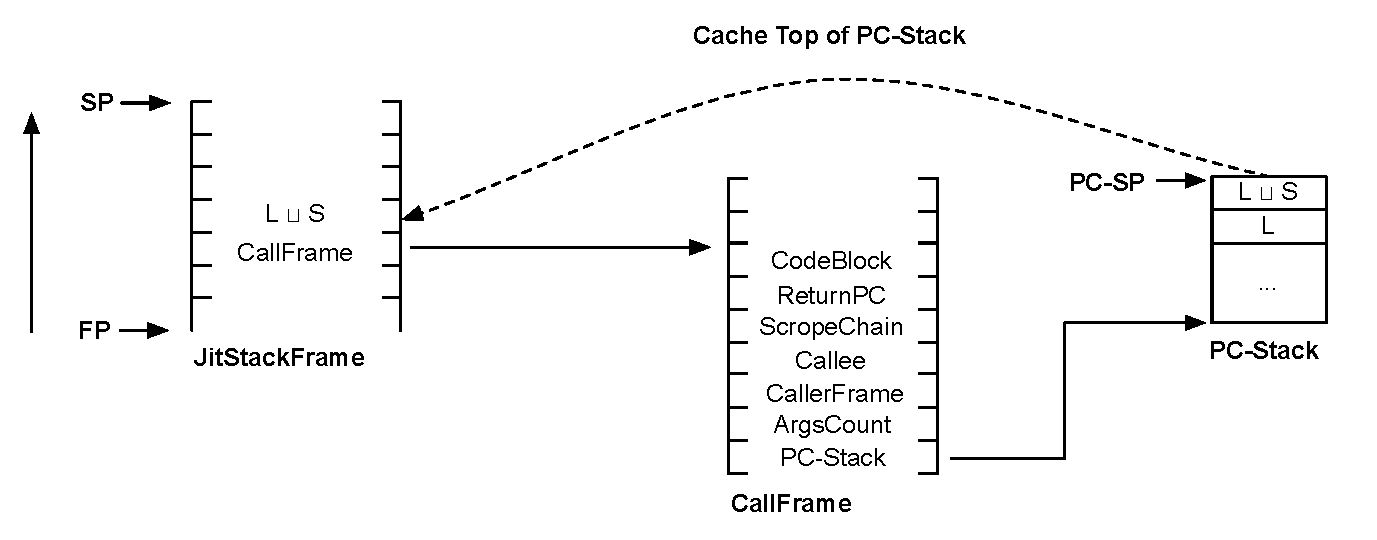
\includegraphics[width=\linewidth,keepaspectratio=true]{graphics/stackframe.pdf}}
  \caption{Interaction of native \code{JITStackFrame}, \code{CallFrame}, and Control-flow stack.}
  \label{fig:jitflow-stackframe}
\end{figure}

\JitFlow\ updates this cache every time the top label of the control-flow stack changes.
This update occurs at control-flow branches and joins and is less frequent than the data-flow operations that access the top label.

Additionally, using such a caching mechanism allows \JitFlow\ to avoid expensive updates on top of the control-flow stack if the label of the predicate and the cached label are identical.
As previously mentioned, the instruction \join\ upgrades the top of the control-flow stack by joining it with the label of the predicate value.
To avoid such unnecessary updates, \JitFlow\ emits compiled code that first checks the equality of the cached label in the \code{JITStackFrame} and the label of the predicate.
If so, the runtime system skips the expensive task of following the pointers to update the top of the control-flow stack because it already holds the correct label.

\item \textit{It implements the instructions that maintain the control-flow stack directly in assembly.}
\JitFlow\ takes as input the same instruction stream as the \FlowCore\ interpreter.
When the JIT compiler encounters one of the control-flow stack manipulation instructions (\autoref{ch:instructions}) it emits assembly code that performs the operation.
Not only does this code access the control-flow stack through the appropriate reference path shown in \autoref{fig:jitflow-stackframe}, but it also updates the cached top label when necessary.
Cache updates only occur in the \join\ and \popj\ instructions, because the \dup\ instruction modifies stack height but does not change the label on top.

Implementing the instructions that maintain the control-flow stack (\dup, \join, and \popj) in assembly code avoids expensive callbacks into C++ at runtime, allowing \JitFlow\ to increase speed by not having to (i) save and restore registers when calling into C++ and (ii) perform the expensive trampoline jump to find the function entry point in C++.

\end{enumerate}

Only by implementing all of these techniques was \JitFlow\ able to achieve the low-overhead performance measured in \autoref{sec:jitflow-evaluation}.

\section{Evaluation}
\label{sec:jitflow-evaluation}

This section evaluates the performance gained by implementing the logic for dynamically tracking information flow in JIT-compiled code.
The techniques used to validate that the implemented logic correctly tracks the flow of information also deserve emphasis.
Finally, I distinguish the limitations that arise as implementation artifacts from the fundamental limitations of the information flow approach.

WebKit contains an interpreter, JavaScriptCore (JSC), that executes a bytecode instruction sequence using direct threaded interpretation\footnote{
In March 2012, JavaScriptCore changed to a low-level interpreter, implemented via a custom language that generates the assembly for a direct threaded interpreter.
The benchmarks shown here measure the performance of the C++ version of JSC that predates this change.
}.
The WebKit project also contains a template JIT compiler that compiles the bytecode instruction stream and an optimizing JIT compiler based on a program's data-flow graph.
\JitFlow\ builds upon the template JIT and does not implement information flow in the optimizing JIT compiler, which operates only on Macintosh operating systems.
All of the following benchmarks compare information flow implementations of interpreter-only and JIT-only execution modes.

\begin{table}[ht]
\centering
\resizebox{\columnwidth}{!}{
\begin{tabular}{r l l l}
\textit{Overhead} & \textit{Language} (implementation) & \textit{Reference}                & \textit{Benchmarks}\\
\toprule
80\%              & JS Interpreter (64~bit labels)     & Kerschbaumer~et~al.~\cite{kerschbaumer.etal+13} & SunSpider\\
100 -- 200\%      & JS Interpreter (64~bit labels)     & Just~et~al.~\cite{just.etal+11}         & V8\\
110 -- 690\%      & JS (rewriting during parse)        & Jang~et~al.~\cite{jang.etal+10}         & meas. by visiting pages\\
120\%             & JS Interpreter (data-flow only)    & Tran~et~al.~\cite{tran.etal+12}         & SunSpider\\
136 -- 560\%      & JS Interpreter (only tags objects) & Dhawan and Ganapathy~\cite{dhawan.ganapath+09}   & SunSpider, V8\\
$\sim$200\%       & JS Interpreter (multi-execution)   & Groef~et~al.~\cite{groef.etal+12}        & V8\\
none reported     & JS Interpreter (1~bit label)       & Vogt~et~al.~\cite{vogt.etal+07}         & no perf numbers given\\

14\%              & Java (data-flow only)              & Enck~et~al.~\cite{enck.etal+10}         & CaffeineMark\\
200\%             & Java (JikesRVM)                    & Chandra~and~Franz~\cite{chandra.franz+07}     & JavaGrande \\

1.6\% -- 26.7\%   & C (instrumenting compiler)         & Nanda~et~al.~\cite{nanda.etal+07}        & LAMP-stack\\
24\% -- 1,120\%   & C (instrumenting compiler)         & Lam~and~Chiueh~\cite{lam.chiueh+06}        & C-Programs\\
1,900\%           & x86 VM                             & Yin~et~al.\cite{yin.etal+07}          & CPU Instruction level tainting\\
\bottomrule
\end{tabular}
}
\caption{Performance Comparison of other Information Flow Frameworks}
\label{tab:jitflow-perfcomparison}
\end{table}

%------------------------------------------------------------------------------------------------------
\subsection{Effect on Performance}
\label{sec:jitflow-evaluation-performance}

To demonstrate how JIT compilation of dynamic information flow tracking reduces the performance impact within an information-flow tracking VM, I execute three established JavaScript benchmark suites:
SunSpider version 1.0~\cite{sunspider}, V8 version~6~\cite{v8}, and Kraken version 1.1~\cite{kraken}.
A dual Quad Core Intel Xeon E5462 2.80~GHz with 9.8~GB RAM running Ubuntu~11.10 (kernel 3.2.0) executes all benchmarks using \texttt{nice~-n~-20} to minimize operating system scheduler effects.
After running each suite once for warm-up, the test software executes 10 repetitions for each benchmark get stable results and reports the geometric mean of these repetitions to discount outliers.
Note that the results for these benchmarks do not include the overhead for JIT compiling the code since this happens during the warm-up run.

Previous implementations of information flow (\autoref{tab:jitflow-perfcomparison}) experience a handicap by beginning with an unmodified interpreter that is already an average of 287\% slower than JIT-compiled code.
On a relative basis, \JitFlow\ outperforms all of the previous work listed in \autoref{tab:jitflow-perfcomparison}.
\JitFlow\ also outperforms on an absolute basis because it is measured with respect to much faster JIT-compiled code.

\begin{figure}[ht]
  \centerline{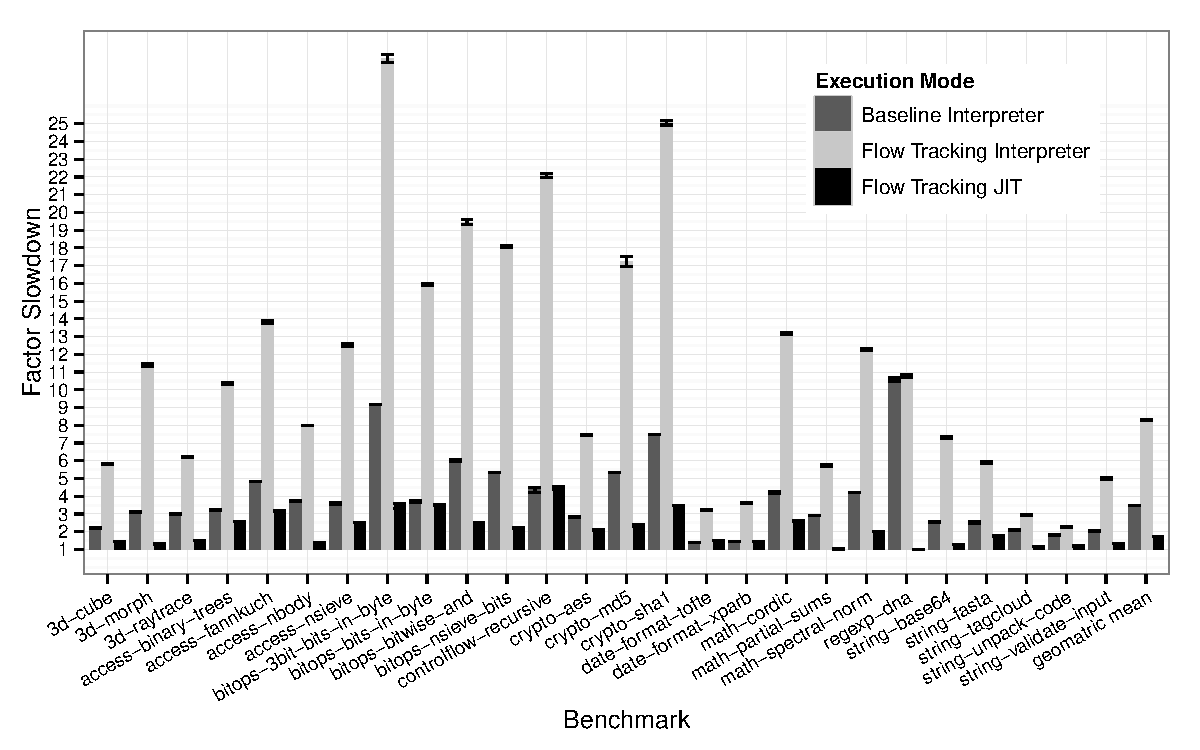
\includegraphics[width=\linewidth,keepaspectratio=true]{graphics/sunspider_plot.pdf}}
  \caption{Detailed performance for the SunSpider benchmark normalized by the \code{JavaScriptCore} JIT compiler.}
   \label{fig:sunspider-performance}
\end{figure}

\begin{figure}[ht]
  \centerline{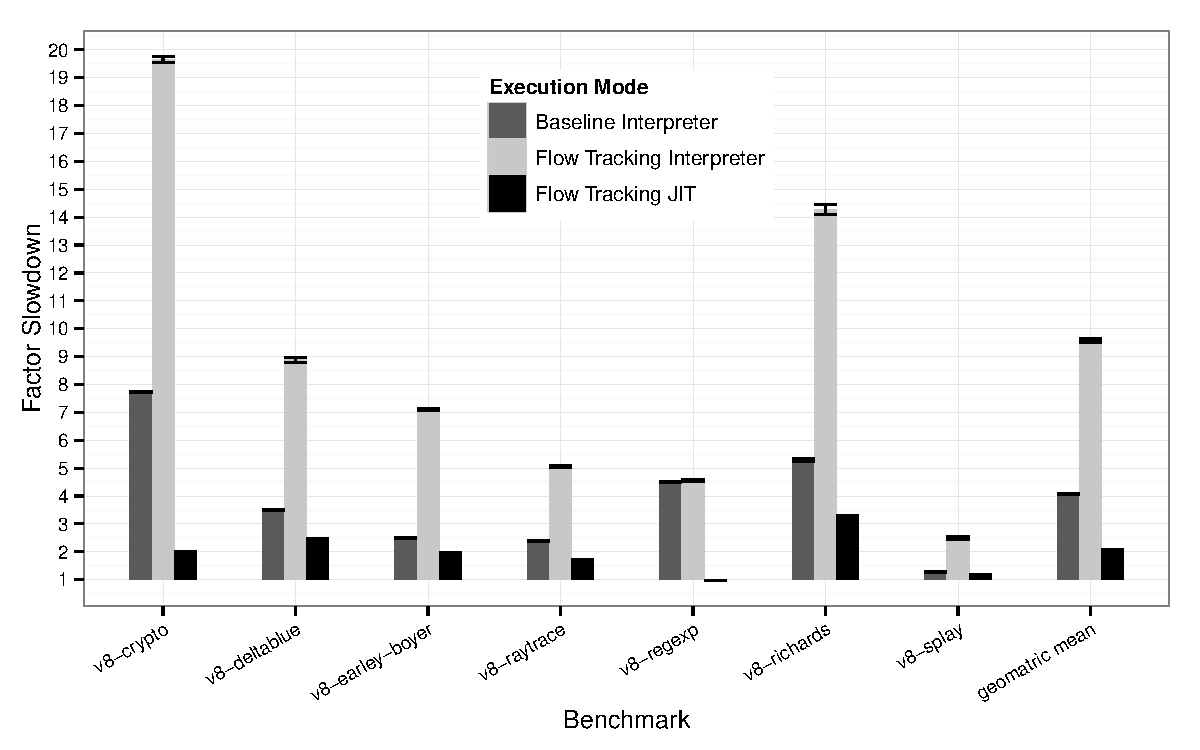
\includegraphics[width=\linewidth,keepaspectratio=true]{graphics/v8_plot.pdf}}
  \caption{Detailed performance for the V8 benchmark normalized by the \code{JavaScriptCore} JIT compiler.}
   \label{fig:v8-performance}
\end{figure}

\begin{figure}[ht]
  \centerline{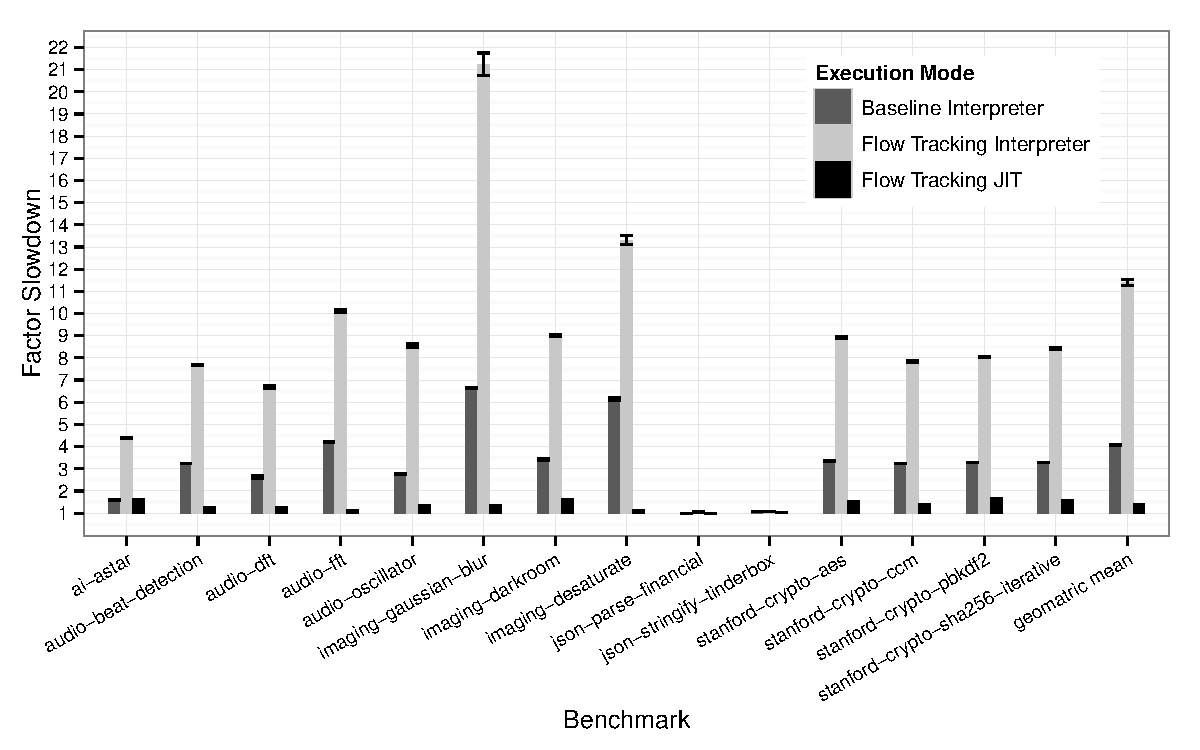
\includegraphics[width=\linewidth,keepaspectratio=true]{graphics/kraken_plot.pdf}}
  \caption{Detailed performance for the Kraken benchmark normalized by the \code{JavaScriptCore} JIT compiler.}
   \label{fig:kraken-performance}
\end{figure}

To provide a consistent basis for performance comparison, I implemented information flow tracking in WebKit's interpreter and JIT compiler using the same label encoding and supporting data structures introduced in \autoref{ch:label-propagation}.
The comparison required creating a 32-bit version of \FlowCore\ that implements inline labels, rather than the fat values discussed previously.
The benchmarks measure the performance of JIT-compiled tracking code (\JitFlow) vs. interpreter code (32-bit \FlowCore) in exclusive modes.
As illustrated in Figures~\ref{fig:sunspider-performance}, \ref{fig:v8-performance}, and \ref{fig:kraken-performance}, the average performance impact for \JitFlow\ (Sunspider~74\%, V8~108\%, and Kraken~38\%) clearly demonstrates that JIT-compiled code implementing dynamic information flow tracking outperforms the execution speed of an unmodified interpreter.
Hence, the \JitFlow\ implementation sets a new bar for dynamic information flow systems.


At the outset, I engineered and incorporated the information flow tracking logic in the JavaScriptCore interpreter, creating \FlowCore.
This effort gave me a deep understanding of WebKit's JavaScript VM and allows a comparison between the relative performance impacts of implementing dynamic information flow tracking in the interpreter vs. the JIT compiler.
Even when implementing information flow in a JIT compiler, the overhead measured as percentage relative to the baseline does not necessarily correspond to that seen when implementing the same framework within the JavaScript interpreter.
For example, the SunSpider benchmark (\autoref{fig:sunspider-performance}) shows an overhead of 137\% in the interpreter, while the JIT compiler shows only 74\%.
A full account of the performance on each individual benchmark (using the encoding and framework as described in \autoref{sec:jitflow-labelencoding}) can be found in \autoref{app:jitflow-detailedresults}.

\todo[inline]{create the appendix of detailed results}

Many of the benchmarks, such as \code{regexp} in V8 and the \code{json} family of tests in Kraken, run with essentially the same speed as the unmodified JIT compiler.
These tests perform fewer control-flow branches and make a higher percentage of native code calls compared to other tests.
Meanwhile, the \code{controlflow-recursive} test in SunSpider introduces the most overhead, at 346\%, because it has a very large number of executed branches in recursive function calls and conditional tests.
These control-flow constructs cause the dynamic information flow VM to perform additional work to maintain the control-flow stack.
Each time the VM recursively calls a function, branches on a conditional, or iterates a loop, it executes the control-flow tracking instructions (\autoref{ch:instructions}), incurring an overhead relative to an unmodified VM.

Overall, the low impact for the JIT-compiled information flow tracking logic (73\% on average, on compute intensive benchmarks) highlights the practicality of dynamic information flow as a security enhancement for the outdated JavaScript security model.

\subsubsection{Impact of Conservatively Labeling Doubles}
\label{sec:jitflow-impact-doubles}

As previously stated in \autoref{sec:jitflow-labelencoding}, the current format of doubles within WebKit does not allow directly encoding a label within the representation of a double.
All operations involving doubles implicitly carry the highest label available at the time they execute.
This conservative labeling strategy might conceal the performance drawback for benchmarks focusing on doubles.

To show that this implementation detail has little performance impact, I report the percentage of operations creating doubles vs. other \jsvalues\ for each of the three benchmark suites.
In SunSpider 4.7\% of \jsvalues\ created are doubles, while in V8 and Kraken fewer than 1\% are doubles, 0.23\% in V8 and 0.96\% in Kraken, respectively.
This ratio lets us conclude that, in those three benchmark suites, doubles account for only a small fragment of created values and therefore do not influence the overall performance impact.

\subsection{Correctness}
\label{sec:jitflow-evaluation-correctness}

To validate that the modifications \JitFlow\ makes to JavaScriptCore's JIT engine for tracking the flow of information throughout execution of a JavaScript program do not introduce any errors, we made sure that none of our modifications broke any of the Mozilla regression tests in the WebKit repository.
This suite consists of over 1,000 test cases covering core JavaScript functionality, including arrays, dates, functions, numbers, objects, regular expressions, and strings.

In addition, I wrote a suite of test cases that check the correct label propagation for the information flow tracking logic and added them to the regression suite.
These tests exercise label propagation for all of the implemented binary operations and control-flow structures: \code{if}-statements, the various loop constructs including break and continue statements, \code{eval}, and function calls.
These these tests make use of a first-class labeling framework~\cite{hennigan.etal+13} (\autoref{ch:first-class-labels}) that permits explicit application and inspection of labels within the JavaScript language itself, allowing the test cases to be incorporated into the regression suite.

\lstset{
  caption={Regression test verifying correct label propagation for additions.},
  label={list:jitflow-regressiontest},
}
\begin{jscode}
var a = (new FlowLabel("labelA"))(24);
var b = (new FlowLabel("labelB"))(12);

var res = a + b;

reportCompare(36, res, "add value incorrect.");
reportCompare(true, (labelof res).subsumes(labelof a),
              "wrong first label in add");
reportCompare(true, (labelof res).subsumes(labelof b),
              "wrong second label in add");

reportCompare((labelof res), (labelof a).join(labelof b),
              "wrong joined label in add");
\end{jscode}

\autoref{list:jitflow-regressiontest} shows one of the crafted regression tests for confirming correct label propagation.
In keeping with the other examples in this paper, this test focuses on the correct label propagation for integer addition.

The integer addition test begins by giving each of the input operands separate labels.
\Codeline{1} assigns input variable \code{a} the value \code{24} with label \code{labelA} (internally mapped to \code{0001}) and \codeline{2} assigns input variable \code{b} the value \code{12} with label \code{labelB} (internally mapped to \code{0010}).

After initialization, the test performs the addition on \codeline{4}.
To provide feedback during development, the test uses the \code{reportCompare} function, provided by the regression suite.
On \codeline{6}, it checks that the result has value \code{36} as expected.

Further sanity checking occurs on \codelines{7}{10} to ensure that the label attached to the result subsumes the label attached to each of the inputs.
Finally, on \codeline{12}, the test verifies that the label attached to the result of the addition (\code{0011}) matches the join of the labels on the operands (\code{0001|0010}).


%------------------------------------------------------------------------------------------------------
\subsection{Real World Applicability}
\label{sec:realworldapplicability}

Conforming to the capabilities of the attacker (Section~\ref{sec:jitflow-thirdpartycode}), this evaluation defines an information flow violation as the inequality of domains between a network data payload and the target.
When the label of the payload indicates that the data has been influenced by any origin other than the destination domain, the network request represents a communication to a foreign party, possibly an attacker-controlled server.

To verify that \JitFlow\ detects information flow violations, a web crawler automatically visits web pages and stays on each web page for 60~seconds.
The web crawler visits a randomly sampled selection 100 of the Alexa~Top~one~million~\cite{alexa} web pages.
To simulate user interaction, the web crawler fills out HTML-forms and submits the first available form on each visited page.
For all of the following results, the crawler used information flow in both the JIT compiler and the interpreter.

\begin{table*}[ht!]
\centering
\resizebox{\columnwidth}{!}{
\begin{tabular}{r|r|l|r || r|l|r}
& \multicolumn{3}{c||}{Ranked by Number of Included Domains} & \multicolumn{3}{c}{Ranked by Number of Flow violations} \\
 & \textit{Alexa Rank} & \textit{Page} & \textit{Dom.}  & \textit{Alexa Rank} & \textit{Page} & \textit{Flows}\\
\hline
1 & 556,895 & \url{prizyvnikmoy.ru} & 13 & 683,716 & \url{onefeat.com} & 295 \\
2 & 540,606 & \url{finn-dinghy.de} & 13 & 592,642 & \url{train-shop.net} & 80 \\\
3 & 438,078 & \url{mitula.ch} & 13 & 196,697 & \url{nudepornstarz.net} & 78 \\
4 & 19,658 & \url{roxio.com} & 13 & 394,557 & \url{just-eat.no} & 51 \\
5 & 999,112 & \url{printertransferroller.blogspot.com} & 12 & 889,993 & \url{sfee.gr} & 49 \\
6 & 799,519 & \url{masteringonlinemarketing.com} & 12 & 801,235 & \url{aksgonline.com} & 37 \\
7 & 683,716 & \url{onefeat.com} & 12 & 556,895 & \url{prizyvnikmoy.ru} & 35 \\
8 & 507,796 & \url{ifm-bonn.org} & 12 & 992,317 & \url{mentoring-uk.org.uk} & 30 \\
9 & 494,397 & \url{natives.co.uk} & 12 & 540,774 & \url{buildinglebow.com} & 27 \\
10 & 472,505 & \url{wcode.ru} & 12 & 834,020 & \url{tct.net.ua} & 24 \\
\hline
& & Average (of all 100 pages)& 7 & & Average (of all 100 pages)& 12 \\
\end{tabular}
}
\caption{Web pages including content from the greatest number of different domains (left) and web pages having the greatest number information flow violations (right).}
\label{tab:webstatistics}
\end{table*}

\subsubsection{Including other domains.}

Modern web applications integrate content from several different origins on the web.
Our statistics show that each of the visited web pages include an average of 7~different origins for their content.
The inline label approach lets \JitFlow\ directly encode up to 16 different domains within one label.
This technique permits an efficient encoding even for the web pages including the most content: \url{prizyvnikmoy.ru}, \url{finn-dinghy.de},  \url{mitula.ch}, and \url{roxio.com} including content from 13 domains.
These findings complement the results of Nikiforakis et al~\cite{nikiforakis.etal+12}, who visited over three million pages for their empirical study showing that more than 90\% of all pages include code from less than 15 different domains.

\subsubsection{Information flow violations}

The \JitFlow\ web crawler first visited the sample of pages using the interpreter and found 1,155 information flow violations.
The page \url{onefeat.com} had the highest observed number of violating flows, at 295.
On average, the crawler detected 12 violating flows per page in our sample (\autoref{tab:webstatistics}).

The crawler revisited the same pages the following day using the JIT compiler and found 1,173 violations.
Because the unit test cases used to develop both the interpreter and JIT compiler implementations attest to the same flow tracking and detection abilities, I attribute the 1.5\% variance between runs to dynamic page content.
For example, the page \url{newsarama.com} increased the number of content requests from 11 to 18 between the two runs, where our network monitor recorded 16 violating information flows in the interpreter and 28 information flow violations in the JIT.
Groef~et~al.~\cite{groef.etal+12} report a similar phenomenon when evaluating their system on real web pages.

The evaluation does not distinguish between malicious flows and detected flow violations due to the presence of Content Distribution Networks (CDNs), which modern web pages use for performance reasons to serve content to their users.
Before \JitFlow\ can be adopted, web site authors need a way to express allowed information flows and whitelist requests to their own CDNs.

\section{Summary}

Today, web users miss out on the increased protection afforded by information flow tracking.
All major browsers include a just-in-time compiler and vendors advertise their performance compared to competitors.
Under these circumstances, implementations of information flow tracking in the JavaScript interpreter are no longer suitable.

\JitFlow\ directly addresses the performance overhead of information flow by implementing the tracking logic in JIT-compiled code.
In spite of the prior work and analysis done to develop \FlowCore, \JitFlow\ does not ``just'' transplant interpretative tracking techniques to a JIT compiler.
Rather, it uses a different encoding that inlines the label for more efficiency with respect to space and time.
To achieve even better performance it (i) optimizes the allocation of the control flow stack to track implicit flows, (ii) it caches the top label of the control flow stack to optimize frequent accesses, and (iii) it inlines the assembly code that maintains the control flow stack to avoiding costly trampoline jumps.
Without these optimizations, a good part of the speedup from JIT compilation would have been lost.

\JitFlow\ has an average tracking overhead of 73\% relative to a baseline JIT compiler on CPU-intensive benchmarks.
On absolute terms, its performance measures more than twice as fast as the fastest known JavaScript information flow tracking interpreter.
In practice, steps such as DNS lookup, parsing and rendering, and content transmission also factor into the browser performance equation.
Consequently, using information flow tracking for realistic web browsing affects the user experience far less than CPU-intensive benchmarks may suggest.
I consider the overhead more than acceptable --- especially since users benefit from substantially increased security in return.

%xxxxxxxxxxxxxxxxxxxxxxxxxxxxxxxxxxxxxxxxxxxxxxxxxxxxxxxxxxxxxxxxxxxx
\todo[inline]{feedback the motivation and thirdpartycode sections of 2013.taco into thesis motivation (pick up more cites)}
\todo[inline]{fix the spacing issue on dup join and popj definitions}
\todo[inline]{check bitwise-or and bitwise-and}
\todo[inline]{globally, control flow stack or control-flow stack?}
\todo[inline]{patch up citations, look at thesis.blg}

\begin{comment}
\chapter{Policies}
  matrx of trade-offs, issues
  outline chart
  real-world frequency of occurance
  - no-sensitive upgrade vs others
\end{comment}

\chapter{Conclusion}
\label{ch:conclusion}

The dynamic approach to information flow tracking in general still has some remaining challenges.
In the case of \JitFlow\ and \FlowCore, these challenges spring from the lack of static analysis available in dynamically typed languages.
For example, when using information flow in the web browser, the security principles do not become known until execution time.
Although, the dynamic approach to information flow approach remains the most suitable option available, some outstanding issues concerning a path to adoption and the details about implementation need addressing.

\section{Adoption of Information Flow in JavaScript}

I identify three roadblocks to the adoption of dynamic information flow systems.
First, the dynamic label upgrading leads to the intrinsic side-effect of label creep~\cite{sabelfeld.myers+03,denning+82}, which results in an unsatisfactory number of policy violations.
Second, web application vary considerably, and no default policy could ever fit the diversity.
Third, users expect all web applications to be responsive to input, no matter how complex the underlying operations.
My experience implementing information flow in JavaScript offers some suggestions to combat label creep, the addition of a feature that helps developers author application specific policies, and an implementation that meets user performance expectations.

\subsection{Addressing Label Creep}

As a JavaScript program executes, labels attached to program values monotonically upgrade through the security principal lattice.
Neither \FlowCore\ nor \JitFlow\ make a strong attempt to stop this behavior.
As observed when surfing the web, \JitFlow\ reported an unsatisfactorily high number of false positive flow violations.

Experience with these systems suggests more research on removing the conservative assumptions through more powerful code analysis.
A strong enough emphasis on security may compel programmers to adopt a language subset.
For example, performance concerns have led to the adoption of asmjs~\cite{asmjs}, a low-level target subset of JavaScript for compilers.
A similar concern for data security within web applications may lead to the adoption of secure subsets such as Caja~\cite{caja}.

Alternatively, any mechanisms that reduce the initial source of high labels ought also to be considered.
Developer may have to consider structuring their programs differently.
After initial release, a later implementation of Jif~\cite{jif} added first-class labels as part of the Java statically-checked type system.
\FlowCore\ and \JitFlow\ also feature a similar mechanism, though without the support for label declassification.

\subsection{Expressing Security Constraints}

In the context of JavaScript and the Web, research lacks strong guidelines for what policies to enforce.
We fully expect that the vast majority web users will find it too difficult to write their own policies to protect their data, and those that can will have little interest in spending the time.
Shipping the browser with a built-in default policy might not be feasible either because web applications vary extensively in both purpose and architecture.
Reports on information leakage~\cite{jang.etal+10,nikiforakis.etal+12,kerschbaumer.etal+13} suggest that, at this time, most sites use visitor data for web site analytics and marketing.

Since I do not have the capacity to know the best security practices for every web application, I can only promote tools that assist the developers.
For example, \JitFlow\ uses a first-class labeling system that allows enforcement any network monitor policy, written by the developer.
The tracking engine can be customized to enforce any policy, so I leave questions of policy creation to other researchers.

\subsection{Reducing Performance Overhead}

Background research into the performance of information flow systems (\autoref{tab:jitflow-perfcomparison}) revealed a substantial overhead.
The development of a control-flow stack and the instructions that manipulate it during the implementation of \FlowCore\ naturally enabled a faster implementation to follow.
By implementing the dynamic tracking logic and control flow stack manipulation in a JIT compiler, \JitFlow\ specifically attacks the performance overhead.
Although the percentual slowdown is still similar to other systems, \JitFlow\ starts from a much faster baseline: the JIT compiled code.
By establishing a new status quo for the implementation of information flow, I hope that more users will be willing to adopt information flow as part of their web browsing experience.

\section{Artifacts Resulting from Implementation}

The implementation of the security data structures that support dynamic information flow tracking result in several limitations that affect the capability of the system.
First, the language itself restricts the types of code analysis that can be used, imposing a fundamental limitation on the kinds of information flow that they system can track.
Second, the bit-vector implementation of labels restricts the number of unique security principals representable in the security lattice.
Finally, the use of a control-flow stack and introduction of new instructions enabled rapid development of \JitFlow\ after implementation of \FlowCore.

\subsection{Flow Tracking Capabilities}

The dynamic information flow tracking used in both \FlowCore\ and \JitFlow\ does not implement passive implicit flow tracking (\autoref{ch:label-propagation}).
Tracking this type of flow requires propagation of control-flow influences through values in non-executed paths and remains an open research question for dynamic languages such as JavaScript.
\FlowCore\ and \JitFlow\ only track information flows through a subset of the JavaScript language definition.
The development effort required for these prototypes implies that covering all language features would require expertise from a JS vendor and a dedicated team of engineers.

\subsection{Representation of Security Principals}

The repurposing of bits within \jsvalues\ limits the \JitFlow\ framework to tracking at most 16 different security principals within a label, while the fat value approach limits the \FlowCore\ framework to 64 different security principles.
The limitation can be overcome in both tracking engines by reserve one or more label bits as a flag to reference a larger label space.
This solution requires a more complex label framework, but offers support for more security principals and a larger lattice~\cite{kerschbaumer.etal+13}.
Results from the web crawler indicate that a limitation on total number of representable security principals is not fundamental.

\subsection{Handoff between the Interpreter and JIT compiler}

The design of the instructions that manipulate the control-flow stack support all the different control structures (switch-case, specialized iteration, exceptions, with statement).
Neither \FlowCore\ nor \JitFlow\ issue these instructions for any structures beyond the basic \code{for} and \code{while} loops, \code{break}, \code{continue}, and \code{if} statements.

An industrial strength implementation requires supporting native data structures (array, string, date, regex, etc.) and property lookup paths (by name, by value, user-overloadable getters/setters, etc.).
The prototypes, \FlowCore\ and \JitFlow\ cover enough operations to demonstrate that the approach to implementation works for both the interpreter and the JIT compiler.

Enough features overlap that the system can be made to support JITting only after the interpreter determines hot code fragments.
I would not expect an on-the-fly translation between interpreter and JIT-compiled code to be a problem, as long as the trampoline mechanism updates the supporting data structures (label lattice and control-flow stack) appropriately.
Indeed, the introduction of the control-flow stack maintenance instructions makes this process easier.

\section{Executive Summary}

\autoref{ch:motivation} gives overview of web architecture and its negative effects on security.
The structure of HTML, dynamic typing of JavaScript, and the textual inclusion of third-party code and data, each contribute to an infrastructure that puts casual web user's data at risk for surreptitious information theft through a code injection attack known as Cross-Site Scripting.
Widespread practice of dynamically creating strings later treated as HTML code defeats static analysis techniques.
To detect and mitigate these attacks, I propose using dynamic information flow to track data propagation in a JavaScript VM, and call the resulting interpreter \FlowCore.

% \todo[inline]{related work is terrible, missing references, repeated paragraphs, mentions firefox}
%\autoref{ch:related-work} provides the research setting in which the \FlowCore\ implementation took place.
%It summarizes prior efforts to establish guidelines and best practices that have been shown to work, and highlights differences that make previous approaches inapplicable to JavaScript.
%The approaches taken by other researchers 
%It contrasts the approach taken by \FlowCore\ with approaches taken by other researchers.
%The implementation 

\autoref{ch:terminology} establishes and names different levels of information flow tracking detail.
The categorization splits information flows between dataflow and control-flow based leaks and correlates each with a required minimum level of program analysis.
Developing this categorization permits a clear definition of the information flow tracking capabilities \FlowCore.
Through dynamic labeling of the program counter, \FlowCore\ can track up to active implicit information flows.

\autoref{ch:system-design} outlines the different implementations \FlowCore\ might have used.
It contrasts the implementation of labels between a fat value approach and a security wrapper approach.
Each approach is assessed based on the provided labelling semantics, the difficulty of implementation,the ease of label access, and the impacts on the garbage collector and other runtime systems.
Based on the outcome of this analysis, \FlowCore\ chooses to implement the fat values value approach for labelling because it (1) provides a reference semantics, (2) does not impact the garbage collector, and (3) easily labels both primitives and object references.

\autoref{ch:label-propagation} describes implementation details that support labeling values within the JavaScript VM.
\FlowCore\ adds a \FlowLabelRegistry\ that stores a lattice over security principals.
The host web browser can dynamically create a security principal for each web domain, accomidating the common practice of loading code and resources from many different domains in one page of a web application.
Each element of the lattice forms a bit-vector that maps to a label.
\FlowCore\ extends the internal representation of JavaScript values to include space for a label.
Propagating information influence from control flow predicates to instructions within the code branch requires the addition of a label stack that tracks changes to the label on the program counter.
As a JavaScript program executes, the labels attached to program values monotonically rise through the lattice, leading to label creep.

\autoref{ch:instructions} introduces three new instructions that maintain the control flow label stack.
A parse-time analysis instruments these instructions into the instruction stream.
In debug mode, an abstract interpretation that explores all control flow paths of the instruction stream ensures correct instrumentation for each method.
During execution, the instructions push, pop, and upgrade the stack according to branches, joins, and loops in the control flow.
The development of these instructions enables a transition in implementation from the interpreter (\FlowCore) to the JIT compiler (\JitFlow).
The instructions are generic enough that they support the grafting of information flow tracking into both register-based (WebKit) and stack-based (Firefox) VM implementations.

\autoref{ch:label-tracking} outlines the semantics and implementation of label propagation that occurs in \FlowCore.
It specifies the label inputs and outputs for mathematical, comparison, and bitwise operations, that occur during data flow operations.
Through illustrative examples, it gives the implementation of label prapagation for JavaScript control-flow features, \code{for} and \code{while} loops, including \code{break} and \code{continue} statements.
These examples demonstrate the placement of the control flow stack instructions.
It describes the label propagation rules for function calls, including the implementation details that affect the control flow stock during function prologue and epilogue.

\autoref{ch:first-class-labels} describes an extension of the labeling framework that gives JavaScript developers access to the labeling system.
\FlowCore\ reflects labels stored in the \FlowLabelRegistry\ as first-class objects into the host environment.
The new \FlowLabelObject\ prototype class enables the creation, comparison, composition of labels, while a new \mlabelof\ keyword enables inspection of labeled variables.
When used with a modified web browser, a network monitor hook allows the writing of a security policy within JavaScript.
Using first-class labels developers can tag specific values with their own labels, decreasing the sources of label creep and using the propagation and inference rules as a security debugging system.
Additionally, the first-class label feature proved invaluable for implementing unittests of the propagation rules and buttressing confidence in the correctness of the implementation.

\autoref{ch:jitflow} demonstrates that the framework developed for the \FlowCore\ interpreter readily supports transition to a JIT compiler.
The new tracking engine, \JitFlow, implements the control-flow stack instructions in assembly, caches the top of the control flow stack in a virtual register, and pre-allocates space for the control flow stack itself.
These optimization lead to a vast performance improvement, that approximately halves the execution time of the flow tracking interpreter.



% These commands fix an odd problem in which the bibliography line
% of the Table of Contents shows the wrong page number.
\clearpage
\phantomsection

%\bibliographystyle{abbrv}
\bibliographystyle{amsalpha}
\bibliography{strdefs,refs,procs}

\appendix

\section{Detailed Benchmark Results}
\label{app:jitflow-detailedresults}

\subsection{Sunspider Benchmark}

\begin{table}[h!]
\centering
\resizebox{\columnwidth}{!}{
\begin{tabular}{l|rr|rr|rr|rr}
\textit{Benchmark} & \textit{Base-JIT} & \textit{\%} & \textit{Base-Int} & \textit{\%} & \FlowCore\ & \textit{\%} & \JitFlow\ & \textit{\%} \\
\toprule
3d&&&&&&&& \\
\quad cube & 12.6 & (0.0) & 28.1 & (123.02) & 73.4 & (482.54) & 18.3 & (45.24) \\
\quad morph & 10.0 & (0.0) & 31.1 & (211.0) & 114.0 & (1040.0) & 13.1 & (31.0) \\
\quad raytrace & 11.3 & (0.0) & 34.1 & (201.77) & 70.4 & (523.01) & 17.0 & (50.44) \\
access&&&&&&&& \\
\quad binary-trees & 3.1 & (0.0) & 10.0 & (222.58) & 32.1 & (935.48) & 8.0 & (158.06) \\
\quad fannkuch & 14.1 & (0.0) & 68.1 & (382.98) & 195.0 & (1282.98) & 44.6 & (216.31) \\
\quad nbody & 8.0 & (0.0) & 29.8 & (272.5) & 64.0 & (700.0) & 11.0 & (37.5) \\
\quad nsieve & 4.0 & (0.0) & 14.3 & (257.5) & 50.1 & (1152.5) & 10.0 & (150.0) \\
bitops&&&&&&&& \\
\quad 3bit-bits-in-byte & 2.4 & (0.0) & 22.0 & (816.67) & 68.8 & (2766.67) & 8.3 & (245.83) \\
\quad bits-in-byte & 6.0 & (0.0) & 22.3 & (271.67) & 95.7 & (1495.0) & 21.1 & (251.67) \\
\quad bitwise-and & 4.0 & (0.0) & 24.1 & (502.5) & 77.8 & (1845.0) & 10.0 & (150.0) \\
\quad nsieve-bits & 6.0 & (0.0) & 32.0 & (433.33) & 108.3 & (1705.0) & 13.2 & (120.0) \\
controlflow&&&&&&&& \\
\quad recursive & 2.8 & (0.0) & 12.2 & (335.71) & 61.8 & (2107.14) & 12.5 & (346.43) \\
crypto&&&&&&&& \\
\quad aes & 9.0 & (0.0) & 25.3 & (181.11) & 67.1 & (645.56) & 18.9 & (110.0) \\
\quad md5 & 3.0 & (0.0) & 16.0 & (433.33) & 51.7 & (1623.33) & 7.1 & (136.67) \\
\quad sha1 & 2.0 & (0.0) & 15.0 & (650.0) & 50.1 & (2405.0) & 7.0 & (250.0) \\
date&&&&&&&& \\
\quad format-tofte & 15.1 & (0.0) & 20.9 & (38.41) & 48.9 & (223.84) & 22.9 & (51.66) \\
\quad format-xparb & 11.0 & (0.0) & 16.1 & (46.36) & 39.9 & (262.73) & 16.0 & (45.45) \\
math&&&&&&&& \\
\quad cordic & 8.0 & (0.0) & 33.6 & (320.0) & 105.5 & (1218.75) & 20.7 & (158.75) \\
\quad partial-sums & 13.0 & (0.0) & 37.9 & (191.54) & 74.5 & (473.08) & 13.4 & (3.08) \\
\quad spectral-norm & 5.0 & (0.0) & 21.0 & (320.0) & 61.4 & (1128.0) & 10.0 & (100.0) \\
regexp&&&&&&&& \\
\quad dna & 15.0 & (0.0) & 158.5 & (956.67) & 161.6 & (977.33) & 15.0 & (0.0) \\
string&&&&&&&& \\
\quad base64 & 8.0 & (0.0) & 20.4 & (155.0) & 58.3 & (628.75) & 10.2 & (27.5) \\
\quad fasta & 9.1 & (0.0) & 22.7 & (149.45) & 53.9 & (492.31) & 16.1 & (76.92) \\
\quad tagcloud & 16.0 & (0.0) & 33.3 & (108.12) & 47.1 & (194.38) & 19.0 & (18.75) \\
\quad unpack-code & 26.1 & (0.0) & 47.7 & (82.76) & 59.2 & (126.82) & 31.1 & (19.16) \\
\quad validate-input & 9.1 & (0.0) & 18.5 & (103.3) & 45.6 & (401.1) & 12.1 & (32.97) \\
\hline
Total (geo mean.) & 233.7 & (0.0) & 815.0 & (248.74) & 1936.2 & (728.5) & 406.6 & (73.98) \\
\bottomrule
\end{tabular}
}
\caption{Detailed performance numbers for Sunspider benchmarks normalized by the unmodified JavaScriptCore JIT compiler.}
\label{tab:jitflow-performance-sunspider}
\end{table}

\newpage
\subsection{V8 Benchmark}

\begin{table}[h!]
\centering
\resizebox{\columnwidth}{!}{
\begin{tabular}{l|rr|rr|rr|rr}
\textit{Benchmark} & \textit{Base-JIT} & \textit{\%} & \textit{Base-Int} & \textit{\%} & \FlowCore\ & \textit{\%} & \JitFlow\ & \textit{\%} \\
\toprule
%v8&&&&&&&& \\
\quad crypto & 239.9 & (0.0) & 1856.2 & (673.74) & 4716.4 & (1865.99) & 482.9 & (101.29) \\
\quad deltablue & 378.7 & (0.0) & 1326.8 & (250.36) & 3362.9 & (788.01) & 932.1 & (146.13) \\
\quad earley-boyer & 171.6 & (0.0) & 427.6 & (149.18) & 1216.5 & (608.92) & 336.5 & (96.1) \\
\quad raytrace & 105.0 & (0.0) & 249.8 & (137.9) & 531.8 & (406.48) & 181.5 & (72.86) \\
\quad regexp & 201.0 & (0.0) & 903.3 & (349.4) & 916.1 & (355.77) & 197.7 & (-1.64) \\
\quad richards & 309.3 & (0.0) & 1637.6 & (429.45) & 4415.4 & (1327.55) & 1015.4 & (228.29) \\
\quad splay & 238.9 & (0.0) & 305.1 & (27.71) & 595.6 & (149.31) & 280.6 & (17.46) \\
\hline
Total (geo. mean) & 1644.4 & (0.0) & 6706.4 & (307.83) & 15754.7 & (858.08) & 3426.7 & (108.39) \\
\bottomrule
\end{tabular}
}
\caption{Detailed performance numbers for V8 benchmarks normalized by the unmodified JavaScriptCore JIT compiler.}
\label{tab:jitflow-performance-v8}
\end{table}

\subsection{Kraken Benchmark}

\begin{table}[h!]
\centering
\resizebox{\columnwidth}{!}{
\begin{tabular}{l|rr|rr|rr|rr}
\textit{Benchmark} & \textit{Base-JIT} & \textit{\%} & \textit{Base-Int} & \textit{\%} & \FlowCore\ & \textit{\%} & \JitFlow\ & \textit{\%} \\
\toprule
ai&&&&&&&& \\
\quad astar & 1567.7 & (0.0) & 2499.4 & (59.43) & 6893.4 & (339.71) & 2484.4 & (58.47) \\
audio&&&&&&&& \\
\quad beat-detection & 648.0 & (0.0) & 2091.1 & (222.7) & 4970.4 & (667.04) & 793.3 & (22.42) \\
\quad dft & 652.5 & (0.0) & 1708.9 & (161.9) & 4357.2 & (567.77) & 807.8 & (23.8) \\
\quad fft & 482.3 & (0.0) & 2035.8 & (322.1) & 4870.5 & (909.85) & 542.3 & (12.44) \\
\quad oscillator & 427.1 & (0.0) & 1177.4 & (175.67) & 3650.1 & (754.62) & 561.4 & (31.44) \\
imaging&&&&&&&& \\
\quad gaussian-blur & 2441.3 & (0.0) & 16186.3 & (563.02) & 51855.2 & (2024.08) & 3298.5 & (35.11) \\
\quad darkroom & 701.7 & (0.0) & 2398.1 & (241.76) & 6309.1 & (799.12) & 1116.2 & (59.07) \\
\quad desaturate & 691.8 & (0.0) & 4249.0 & (514.19) & 9205.9 & (1230.72) & 785.1 & (13.49) \\
json&&&&&&&& \\
\quad parse-financial & 85.1 & (0.0) & 83.5 & (-1.88) & 89.4 & (5.05) & 84.8 & (-0.35) \\
\quad stringify-tinderbox & 102.0 & (0.0) & 107.7 & (5.59) & 108.9 & (6.76) & 104.9 & (2.84) \\
stanford&&&&&&&& \\
\quad crypto-aes & 215.6 & (0.0) & 723.6 & (235.62) & 1923.0 & (791.93) & 322.6 & (49.63) \\
\quad crypto-ccm & 168.8 & (0.0) & 544.9 & (222.81) & 1322.1 & (683.23) & 235.6 & (39.57) \\
\quad crypto-pbkdf2 & 533.1 & (0.0) & 1746.4 & (227.59) & 4287.2 & (704.2) & 869.3 & (63.07) \\
\quad crypto-sha256-iterative & 166.4 & (0.0) & 547.3 & (228.91) & 1401.9 & (742.49) & 260.5 & (56.55) \\
\hline
Total (geo. mean) & 8883.4 & (0.0) & 36099.4 & (306.37) & 101244.3 & (1039.7) & 12266.7 & (38.09) \\
\bottomrule
\end{tabular}
}
\caption{Detailed performance numbers for Kraken benchmarks normalized by unmodified JavaScriptCore JIT compiler.}
\label{tab:jitflow-performance-kraken}
\end{table}


\end{document}
